\mainmatter

\chapter{Introduction}
\label{cha:introduction}
When analyzing complex dynamical systems, such as nonlinear many-body problems,
the conventional approach to predicting future states by means of simulating
the trajectories of point particles is frequently insufficient. This is due
to the resulting predictions being very sensitive to small changes in time
and initial positions. One way of addressing the delicate dependence on initial
conditions is to run several different models for the same underlying physical
systems. This invariably results in larger, more well-resolved distributions
of the transported particles, at the cost of ignoring key, inherent, organizing
structures in the system.

Recently, the concept of Lagrangian coherent structures saw the light of day,
emerging from the intersection between nonlinear dynamics, that is, the
underlying mathematical principles of chaos theory, and fluid dynamics. These
provide a new framework for understanding transport phenomena in concept
fluid flow systems. Lagrangian coherent structures can be described as
time-evolving `landscapes' in a multidimensional space, which dictate flow
patterns in dynamical systems. In particular, such structures define the
interfaces of dynamically distinct, invariant regions. An invariant region is
characterized as a domain where all particle trajectories that originate within
the region, remain in it, although the region itself can move and deform with
time. So, simply put; Lagrangian coherent structures enable us to make
predictions regarding the future states of flow systems.

There are two possible ways of describing fluid flow. The Eulerian approach
is to consider the properties of a flow field at each fixed point in time and
space. An example is the concept of velocity fields, which produce the
local and instantaneous velocities of all fluid elements within the domain
under consideration. The Lagrangian point of view, on the other hand, concerns
the developing velocity of each individual particle along their paths, as they
are transported by the flow. Unlike the Eulerian perspective, the Lagrangian
mindset is objective, as in frame-invariant. That is, properties of Lagrangian
fields are unchanged by time-dependent translations and rotations of the
reference frame. For unsteady flow systems, which are more common than
steady flow systems in nature, there exists no self-evident preferred frame
of reference. This means that any transport-dictating dynamic structures
should hold for \emph{any} choice of reference frame. Furthermore, this is
the main rationale for which \emph{Lagrangian}, rather
than \emph{Eulerian}, coherent structures have been pursued.

Although the framework for detecting Lagrangian coherent structures is
mathematically valid for any number of dimensions, the focus of this project
work has been two-dimensional flow systems. Many natural processes fall
within this category, perhaps most notably the transport of debris and
contaminations, such as radioactive particles or the remnants of an oil
spill, by means of oceanic surface currents. Being able to successfully predict
where such particles will be taken by the flow enables us to isolate and
extract them before they are able to reach the coastline, thus preventing
potential humanitarian and natural calamities.

\newpage

At the heart of detecting Lagrangian coherent structures lies the advection
of fluid elements by means of a velocity field, which describes the system
under consideration. This rings true both for test cases, where the velocity
profile is known analytically, and for real-life systems, typically described
by means of discrete samples of the instantaneous velocity field. For this
project work, the topic of interest is how the detection of Lagrangian coherent
structures depends on the choice of numerical integration method used in order
to compute the aforementioned particle transport. In particular, four singlestep
methods and four embedded, adaptive step length methods, each with different
properties, were used in order to advect a collection of fluid elements
by means of an analytically known, two-dimensional, unsteady velocity field.




%\begin{framed}
%    \begin{itemize}
%        \item \sout{Lagrangian coherent structure: A structure that can separate dynamically
%            distinct invariant regions. Invariant retions: All trajectories starting
%            out within it, remains within the region, although the region itself
%        may move and deform with time.}
%    \item \sout{Lagrangian coherent structure: Landscapes in multidimensional
%        landscapes, shaping the flow patterns in dynamical systems.}
%    \item \sout{Motivation: Complex systems, i.e., many-particle nonlinear
%        systems: Need computational shortcuts}
%    \item \sout{LCS: Principally robust structures which enable us
%                        to make predictions regarding the future states of
%                    a flow system.}
%                \item \sout{Examples of real-world application:}
%                            \begin{itemize}
%                                \item \sout{Population growth}
%                                \item \sout{Predicting the advection of particles by means of oceanic currents or wind}
%    \begin{itemize}
%        \item \sout{Recent examples: The volcanic eruptions at Eyafjällajökul, and
%            at Bali (2017)}
%    \end{itemize}
%\item \sout{Predicting where the remnants of an oil spill will end up --> Where to focus
%    the rescue operation in the short and medium term}
%                            \end{itemize}
%    \end{itemize}
%\end{framed}


\vspace{\fill}

\newpage

\chapter{Theory}
\label{cha:theory}
\section[Solving systems of ordinary differential equations]%
{Solving systems of ordinary differential eq\hspace{0em}uations}
\label{sec:solvingsystems}

In physics, like other sciences, modeling a system often equates to solving
an initial value problem. An initial value problem can be described in terms
of a differential equation of the form
\begin{equation}
    \label{eq:ivpsystem}
    \dot{x}(t) = f\big(t,x(t)\big),\quad{}x(t_{0})=x_{0},
\end{equation}
where $x$ is an unknown function (scalar or vector) of time $t$. The function
$f$ is defined on an open subset $\Omega$ of $\mathbb{R}\times\mathbb{R}^{n}$.
The initial condition $(t_{0},x_{0})$ is a point in the domain of $f$, i.e.,
$(t_{0},x_{0})\in\Omega$. In higher dimensions (i.e., $n>1$) the differential
equation~\eqref{eq:ivpsystem} is replaced by a family of equations
\begin{equation}
\label{eq:ivpsystemhigherdimensions}
\begin{gathered}
    \dot{x}_{i}(t) = f_{i}\big(t,x_{1}(t),x_{2}(t),\ldots,x_{n}(t)\big),\quad
    x_{i}(t_{0})=x_{i,0},\quad{}i=1,\ldots,n. \\
\end{gathered}
\end{equation}
The system if nonlinear if the function $f$ in equation~\eqref{eq:ivpsystem},
or, if at least one of the functions $f_{i}$ in equation
\eqref{eq:ivpsystemhigherdimensions}, is nonlinear in one or more of its
arguments.

\subsection{The Runge-Kutta family of numerical methods}
\label{sub:the_runge_kutta_family_of_numerical_methods}

For nonlinear systems, analytical solutions frequently do not exist. Thus, such
systems are often analyzed by means of numerical methods. In numerical analysis,
the Runge-Kutta family of methods are a popular collection of implicit
and explicit iterative methods, used in temporal discretization in order to
obtain numerical approximations of the \emph{true} solutions of systems like
\eqref{eq:ivpsystem}. The German mathematicians C. Runge and M. W. Kutta
developed the first of the family's methods at the turn of the twentieth century
\parencite[p.134]{hairer1993solving}. The general scheme of
what is now known as a Runge-Kutta method is as follows: \\

\begin{defn}
    \label{def:generalrungekutta}
    Let $s$ be an integer and $a_{1,1},a_{1,2},\ldots,a_{1,s},a_{2,1},
    a_{2,2},\ldots,a_{2,s},\ldots,a_{s,1},a_{s,2},\ldots,a_{s,s}$,
    $b_{1},b_{2},\ldots,b_{s}$ and $c_{1},c_{2},\ldots,c_{s}$ be real
    coefficients. Let $h$ be the numerical step length used in the
    temporal discretization. Then, the method
\begin{equation}
    \label{eq:generalrungekutta}
    \begin{aligned}
        k_{i} &= f\bigg(t_{n}+c_{i}h,x_{n}+
                h\sum\limits_{j=1}^{s}a_{i,j}k_{j}\bigg),\quad{}i=1,\ldots,s\\
        x_{n+1} &= x_{n} + h\sum\limits_{i=1}^{s}b_{i}k_{i}
    \end{aligned}
\end{equation}
is called an \emph{s-stage Runge-Kutta method} for the system
\eqref{eq:ivpsystem}.
\end{defn}


The main reason to include multiple stages $s$ in a Runge-Kutta method,
is to improve the numerical accuracy of the computed solutions.
\textcite[p.134]{hairer1993solving} define the \emph{order}
of a Runge-Kutta method as follows:\\

\begin{defn}
    \label{def:rungekuttaorder}
    A Runge-Kutta method \eqref{eq:generalrungekutta} is said to be of
    \emph{order} $p$ if, for sufficiently smooth systems \eqref{eq:ivpsystem},
    \begin{equation}
        \label{eq:rungekuttaorder}
        \norm{x_{n+1}-x(t_{n+1})} \leq Kh^{p+1},
    \end{equation}
    where $K$ is a numerical constant, i.e., if the Taylor series for the exact
    solution $x(t_{n+1})$ and the numerical solution $x_{n+1}$ coincide up to
    (and including) the term $h^p$.
\end{defn}

It is easy to show that if the local error of a Runge-Kutta method is of order
$p+1$, the global error, i.e., the total accumulated error resulting of
applying the algorithm a number of times, is expected to scale as $h^{p}$.
Showing this is left as an exercise for the interested reader.

In definition~\ref{def:generalrungekutta}, the matrix $(a_{i,j})$ is commonly
called the \emph{Runge-Kutta matrix}, while $b_{i}$ and $c_{i}$ are known as
the \emph{weights} and \emph{nodes}, respectively.  Since the 1960s, it has
been customary to represent Runge-Kutta methods~\eqref{eq:generalrungekutta}
symbolically, by means of mnemonic devices known as Butcher tableaus
\parencite[p.134]{hairer1993solving}. The Butcher tableau
for a general \emph{s}-stage Runge-Kutta method, introduced in definition
\ref{def:generalrungekutta}, is presented in table~\ref{tab:generalbutcher}.

\begin{table}[htpb]
    \centering
    \caption[Butcher tableau representation of a general $s$-stage
                Runge-Kutta method]{Butcher tableau representation of a general
                    $s$-stage Runge-Kutta method.}
    \label{tab:generalbutcher}
    \[\renewcommand{\arraystretch}{1.25}
        \begin{array}{c|cccc}
            \toprule
            c_{1} & a_{1,1} & a_{1,2} & \ldots & a_{1,s}\\
            c_{2} & a_{2,1} & a_{2,2} & \ldots & a_{2,s}\\
            \vdots & \vdots & \vdots & \ddots & \vdots \\
            c_{s} & a_{s,1} & a_{s,2} & \ldots & a_{s,s}\\
            \hline
            & b_{1} & b_{2} & \ldots & b_{s}\\
            \bottomrule
    \end{array}
\]
\end{table}

For explicit Runge-Kutta methods, the Runge-Kutta matrix $(a_{i,j})$ is lower
triangular. Similarly, for fully implicit Runge-Kutta methods, the Runge-Kutta
matrix is upper triangular. Unlike explicit methods, implicit methods require
the solution of a linear system at every time level, making them more
computationally demanding than their explicit siblings. The main selling point
of implicit methods is that they are more numerically stable than explicit
methods. This property means that implicit methods are particularly well-suited
for \emph{stiff} systems, i.e., physical systems with highly disparate time
scales~\parencite[p.2]{hairer1996solving}. For such systems,
most explicit methods are highly numerically unstable, unless the numerical step
size is made exceptionally small, rendering most explicit methods practically
useless. For \emph{nonstiff} systems, however, implicit methods behave similarly
to their explicit analogues in terms of numerical accuracy and
convergence properties.

\clearpage

During the first half of the twentieth century, a substantial amount of research
was conducted in order to develop numerically robust, high-order, explicit
Runge-Kutta methods. The idea was that using such methods would mean one could
resort to larger time increments $h$ without sacrificing precision in the
computational solution. However, the number of stages $s$ grows quicker than
linearly as a function of the required order $p$. It has been proven
that, for $p\geq5$, no explicit Runge-Kutta method of order $p$ with $s=p$
stages exists \parencite[p.173]{hairer1993solving}. This is
one of the reasons for the attention shift from the latter half of the 1950s
and onwards, towards so-called \emph{embedded} Runge-Kutta methods.

The basic idea of embedded Runge-Kutta methods is that they, aside from the
numerical approximation $x_{n+1}$, yield a second approximation
$\widehat{x}_{n+1}$. The difference between the two approximations then yields
an estimate of the local error of the less precise result, which can be used for
automatic step size control. The trick is to construct two independent, explicit
Runge-Kutta methods which both use the \emph{same} function evaluations. This
results in practically obtaining the two solutions for the price of one, in
terms of computational complexity. The Butcher tableau of an embedded, general,
explicit Runge-Kutta method is illustrated in
\cref{tab:generalembeddedbutcher}.

\begin{table}[htpb]
    \centering
    \caption[Butcher tableau representation of general, embedded, explicit
    Runge-Kutta methods]{Butcher tableau representation of general, embedded,
        explicit Runge-Kutta methods.}
    \label{tab:generalembeddedbutcher}
    \[\renewcommand{\arraystretch}{1.25}
    \begin{array}{c|ccccc}
    \toprule
    0 \\
    c_{2} & a_{2,1} \\
    c_{3} & a_{3,1} & a_{3,2} \\
    \vdots & \vdots & \vdots & \ddots\\
    c_{s} & a_{s,1} & a_{s,2} & \ldots & a_{s,s-1}\\
    \hline
    & b_{1} & b_{2} & \ldots & b_{s-1} & b_{s} \\
    \hline
    & \widehat{b}_{1} & \widehat{b}_{2} & \ldots & \widehat{b}_{s-1}& \widehat{b}_{s}\\
    \bottomrule
    \end{array}
\]
\end{table}

For embedded methods, the coefficients are tuned such that
\begin{subequations}
    \begin{equation}
        \label{eq:embeddedsol}
        x_{n+1} = x_{n} + h\sum\limits_{i=1}^{s}b_{i}k_{i}
    \end{equation}
is of order $p$, and
    \begin{equation}
        \label{eq:embeddedinterp}
        \widehat{x}_{n+1} = x_{n} + h\sum\limits_{i=1}^{s}\widehat{b}_{i}k_{i}
    \end{equation}
\end{subequations}
is of order $\widehat{p}$, typically with $\widehat{p} = p \pm 1$.

\clearpage

\subsection{The Runge-Kutta methods under consideration}
\label{sub:the_runge_kutta_methods_under_consideration}

Naturally, an abundance of Runge-Kutta methods exist. Many of them are
fine-tuned for specific constraints, such as problems of varying degrees of
stiffness. It is neither possible nor meaningful to investigate them all
in the context of general flow dynamics. For this reason, I consider two classes
of explicit Runge-Kutta methods, namely singlestep and adaptive stepsize
methods. From both classes, I include four different general-purpose ODE solvers
of varying order.

\subsubsection{Singlestep methods}
\label{ssub:singlestep_methods}

The singlestep methods under consideration are the classical, explicit
Runge-Kutta methods of orders one through to four, i.e., the \emph{Euler},
\emph{Heun}, \emph{Kutta} and \emph{classical Runge-Kutta} methods. The
Euler method is \nth{1} order accurate, and requires a single function
evaluation of the right hand side of the ordinary differential equation
\eqref{eq:ivpsystem} or~\eqref{eq:ivpsystemhigherdimensions} at each time step.
Its Butcher tableau representation can be found in~\cref{tab:butchereuler}.
It is the simplest explicit method for numerical integration of ordinary
differential equations. The Euler method is often used as a basis to construct
more complex methods, such as the Heun method, which is also known as the
\emph{improved Euler method} or the \emph{explicit trapezoidal rule}. The Heun
method is \nth{2} order accurate, and requires two function evaluations at each
time step. Its Butcher tableau representation can be found in
\cref{tab:butcherrk2}.

\begin{figure}[htpb]
    \centering
    \input{figures/lcs_figures/euler.pgf}
    \caption[LCS curves found by means of the Euler integration scheme]{
        LCS curves found by means of the Euler integration scheme. The
        reference LCS, as shown by itself in figure~\ref{fig:referencelcs},
        is plotted on the bottom layer. There is a clearly visible offset
        compared to the reference, for all but the two smallest numerical step
        lengths considered. The two latter LCS curves appear to conform well.}
    \label{fig:lcs_euler}
\end{figure}


\begin{figure}[htpb]
    \centering
    \input{figures/lcs_figures/rk2.pgf}
    \caption[LCS curves found by means of the Heun integration scheme]{
        LCS curves found by means of the Heun integration scheme. The
        reference LCS, as shown by itself in figure~\ref{fig:referencelcs},
        is dashed on the top layer. There exists discrepancies with
        regards to the reference for the two largest numerical time step
        lengths considered. These are most prominent in the lower left corner,
        and near $x=1$.}
    \label{fig:lcs_rk2}
\end{figure}


The Kutta method is \nth{3} order accurate, and requires three function
evaluations of the right hand side of the ordinary differential equation
\eqref{eq:ivpsystem} or ~\eqref{eq:ivpsystemhigherdimensions} at each time
step. Its Butcher tableau representation can be found in \cref{tab:butcherrk3}.
The classical Runge-Kutta method is \nth{4} order accurate, and perhaps the most
well-known and frequently used of the four singlestep schemes discussed in this
project. One reason for its popularity is that it is exceptionally stable
numerically (i.e., of the aforementioned singlestep methods, the classical
Runge-Kutta method has the largest numerical stability domain). Another is that,
as mentioned previously, for $p\geq5$, no explicit Runge-Kutta method of order
$p$ with $s=p$ stages exist
\parencite[p.173]{hairer1993solving} -- in other words,
the required number of function evaluations grows at a disproportional rate with
the required accuracy order. For systems with right hand sides which are
computationally costly to evaluate, this means that one frequently is able to
obtain the desired numerical accuracy more effectively by using, for instance,
the classical Runge-Kutta method with a finer step length. The Butcher tableau
representation of the classical Runge-Kutta method can be found in
\cref{tab:butcherrk4}.

\begin{figure}[htpb]
    \centering
    \input{figures/lcs_figures/rk3.pgf}
    \caption[LCS curves found by means of the Kutta integration scheme]{
        LCS curves found by means of the Kutta integration scheme. The
        reference LCS, as shown in figure~\ref{fig:referencelcs},
        is dashed on the top layer. There are some disparities with
        regards to the reference both for the two largest numerical
        time step lengths considered. These are most pronounced in the lower
        left corner, near the leftmost `$\cup$' shape by $y=0.4$ and the
        `$\cap$' shape near $x=1.25$.}
    \label{fig:lcs_rk3}
\end{figure}


\begin{figure}[htpb]
    \centering
    \input{figures/lcs_figures/rk4.pgf}
    \caption[LCS curves found by means of the classical Runge-Kutta integration scheme]{
        LCS curves found by means of the classical Runge-Kutta integration scheme. The
        reference LCS, as shown by itself in figure~\ref{fig:referencelcs},
        is dashed on the top layer. One of the very few visible
        discrepancies belongs to the second largest numerical time step length
        considered, and is located in the lower left corner.}
    \label{fig:lcs_rk4}
\end{figure}


\subsubsection{Adaptive stepsize methods}
\label{ssub:adaptive_stepsize_methods}

The adaptive stepsize methods under consideration are the Bogacki-Shampine
3(2) and 5(4) methods, and the Dormand-Prince 5(4) and 8(7) methods. The digit
outside of the parentheses indicates the order of the solution which is used
to continue the integration, while the digit within the parentheses indicates
the order of the interpolant solution. Note that the concept of \emph{order}
does not translate directly from singlestep methods, as a direct consequence
of the adaptive time step. Generally, lower order methods are more
suitable than higher order methods for cases where crude approximations of the
solution are sufficient. Bogacki and Shampine argue that their methods
outperform other methods of the same order
\parencite{bogacki1989pair,bogacki1996efficient}, a notion which, for the 5(4)
method, is supported by
\textcite[p.194]{hairer1993solving}.

Butcher tableau representations of the aforementioned adaptive stepsize methods
can be found in
\cref{tab:butcherbs32,tab:butcherbs54,tab:butcherdopri54,tab:butcherdopri87},
the latter of which has been typeset in landscape orientation for the reader's
convenience. Three of the methods, namely the Bogacki-Shampine 3(2) and 5(4)
methods, in addition to the Dormand-Prince 5(4) method, possess the so-called
\emph{First Same As Last} property. This means that the last function evaluation
of an accepted step is exactly the same as the first function evaluation of the
next step. This is readily apparent from their Butcher tableaus, where the
$b$ coefficients correspond exactly with the last row the Runge-Kutta matrix.
The \emph{First Same As Last} property reduces the computational
cost of a successive step.

\begin{table}[htpb]
    \centering
    \caption[Butcher tableau representation of the Bogacki-Shampine 3(2)
    embedded Runge-Kutta method]{Butcher tableau representation of the Bogacki-
    Shampine 3(2) embedded Runge-Kutta method. The $b$ coefficients correspond
to a \nth{3}-order accurate solution used to continue the integration. The
$\widehat{b}$ coefficients correspond to a \nth{2}-order accurate interpolant,
which can be used to estimate the error of the numerical approximation, and to
dynamically adjust the time step. The \emph{First Same As Last} property is
apparent from the fact that the $b$ coefficients correspond exactly to the
last row of coefficients in the Runge-Kutta matrix. For reference, see
\textcite{bogacki1989pair}.}
    \label{tab:butcherbs32}
    \renewcommand{\arraystretch}{2.5}
    \begin{tabular}{C|CCCC}
        \toprule
        0 & \\
        \dfrac{1}{2} & \dfrac{1}{2} \\
        \dfrac{3}{4} & 0 & \dfrac{3}{4} \\
        1 & \dfrac{2}{9} & \dfrac{1}{3} & \dfrac{4}{9} \\
        \hline
        & \dfrac{2}{9} & \dfrac{1}{3} & \dfrac{4}{9} \\
        \hline
        & \dfrac{7}{24} & \dfrac{1}{4} & \dfrac{1}{3} & \dfrac{1}{8} \\
        \bottomrule
    \end{tabular}
\end{table}


\vspace{\fill}

\begin{table}[htpb]
\centering
    \caption[Butcher tableau representation of the Bogacki-Shampine 5(4)
    embedded Runge-Kutta method]{Butcher tableau representation of the Bogacki-
    Shampine 5(4) embedded Runge-Kutta method. The $b$ coefficients correspond
to a \nth{5} order accurate solution used to continue the integration. The
two rows of $\widehat{b}$ coefficients correspond to two independent \nth{4}
order accurate interpolants. They can be used to estimate the error of the
numerical approximation, and to dynamically adjust the time step. The fact that
two independent interpolants are included is a part of the reason for which
the method nearly behaves like a \nth{6} order method
\parencite[p.194 in the 2008 printing]{hairer1993solving}. The
\emph{First Same As Last} property is apparent from the fact that the $b$
coefficients correspond exactly to the last row of coefficients in the
Runge-Kutta matrix. For reference, see~\textcite{bogacki1996efficient}.}
    \label{tab:butcherbs54}
    \renewcommand{\arraystretch}{2.5}
    \begin{tabular}{C|CCCCCCCC}
        \toprule
        0 & \\
        \dfrac{1}{6} & \dfrac{1}{6} \\
        \dfrac{2}{9} & 0 & \dfrac{2}{27} & \dfrac{4}{27} \\
        \dfrac{3}{7} & \dfrac{183}{1372} & \dfrac{-162}{343} %
                     & \dfrac{1053}{1372} \\
        \dfrac{2}{3} & \dfrac{68}{297} & \dfrac{-4}{11} & \dfrac{42}{143} %
                     & \dfrac{1960}{3861} \\
        \dfrac{3}{4} & \dfrac{597}{22528} & \dfrac{81}{352} %
                     & \dfrac{63099}{585728} & \dfrac{58653}{366080} %
                     & \dfrac{4617}{20480} \\
        1 & \dfrac{174197}{959244} & \dfrac{-30942}{79937} %
          & \dfrac{8152137}{19744439} & \dfrac{666106}{1039181} %
          & \dfrac{-29421}{29068} & \dfrac{482048}{414219} \\
        1 & \dfrac{587}{8064} & 0 & \dfrac{4440339}{15491840} %
          & \dfrac{24353}{124800} & \dfrac{387}{44800} & \dfrac{2152}{5985} %
          & \dfrac{7267}{94080} \\
        \hline
          & \dfrac{587}{8064} & 0 & \dfrac{4440339}{15491840} %
          & \dfrac{24353}{124800} & \dfrac{387}{44800} & \dfrac{2152}{5985} %
          & \dfrac{7267}{94080} \\
        \hline
        & \dfrac{6059}{80640} & 0 & \dfrac{8559189}{30983680} %
        & \dfrac{26411}{124800} & \dfrac{-927}{89600} & \dfrac{443}{1197} %
                              & \dfrac{7267}{94080} \\
        & \dfrac{2479}{34992} & 0 & \dfrac{123}{416} & \dfrac{612941}{3411720} %
        & \dfrac{43}{1440} & \dfrac{2272}{6561} & \dfrac{79937}{1113912} %
        & \dfrac{3293}{556956} \\
        \bottomrule
    \end{tabular}
\end{table}


\begin{figure}[htpb]
    \centering
    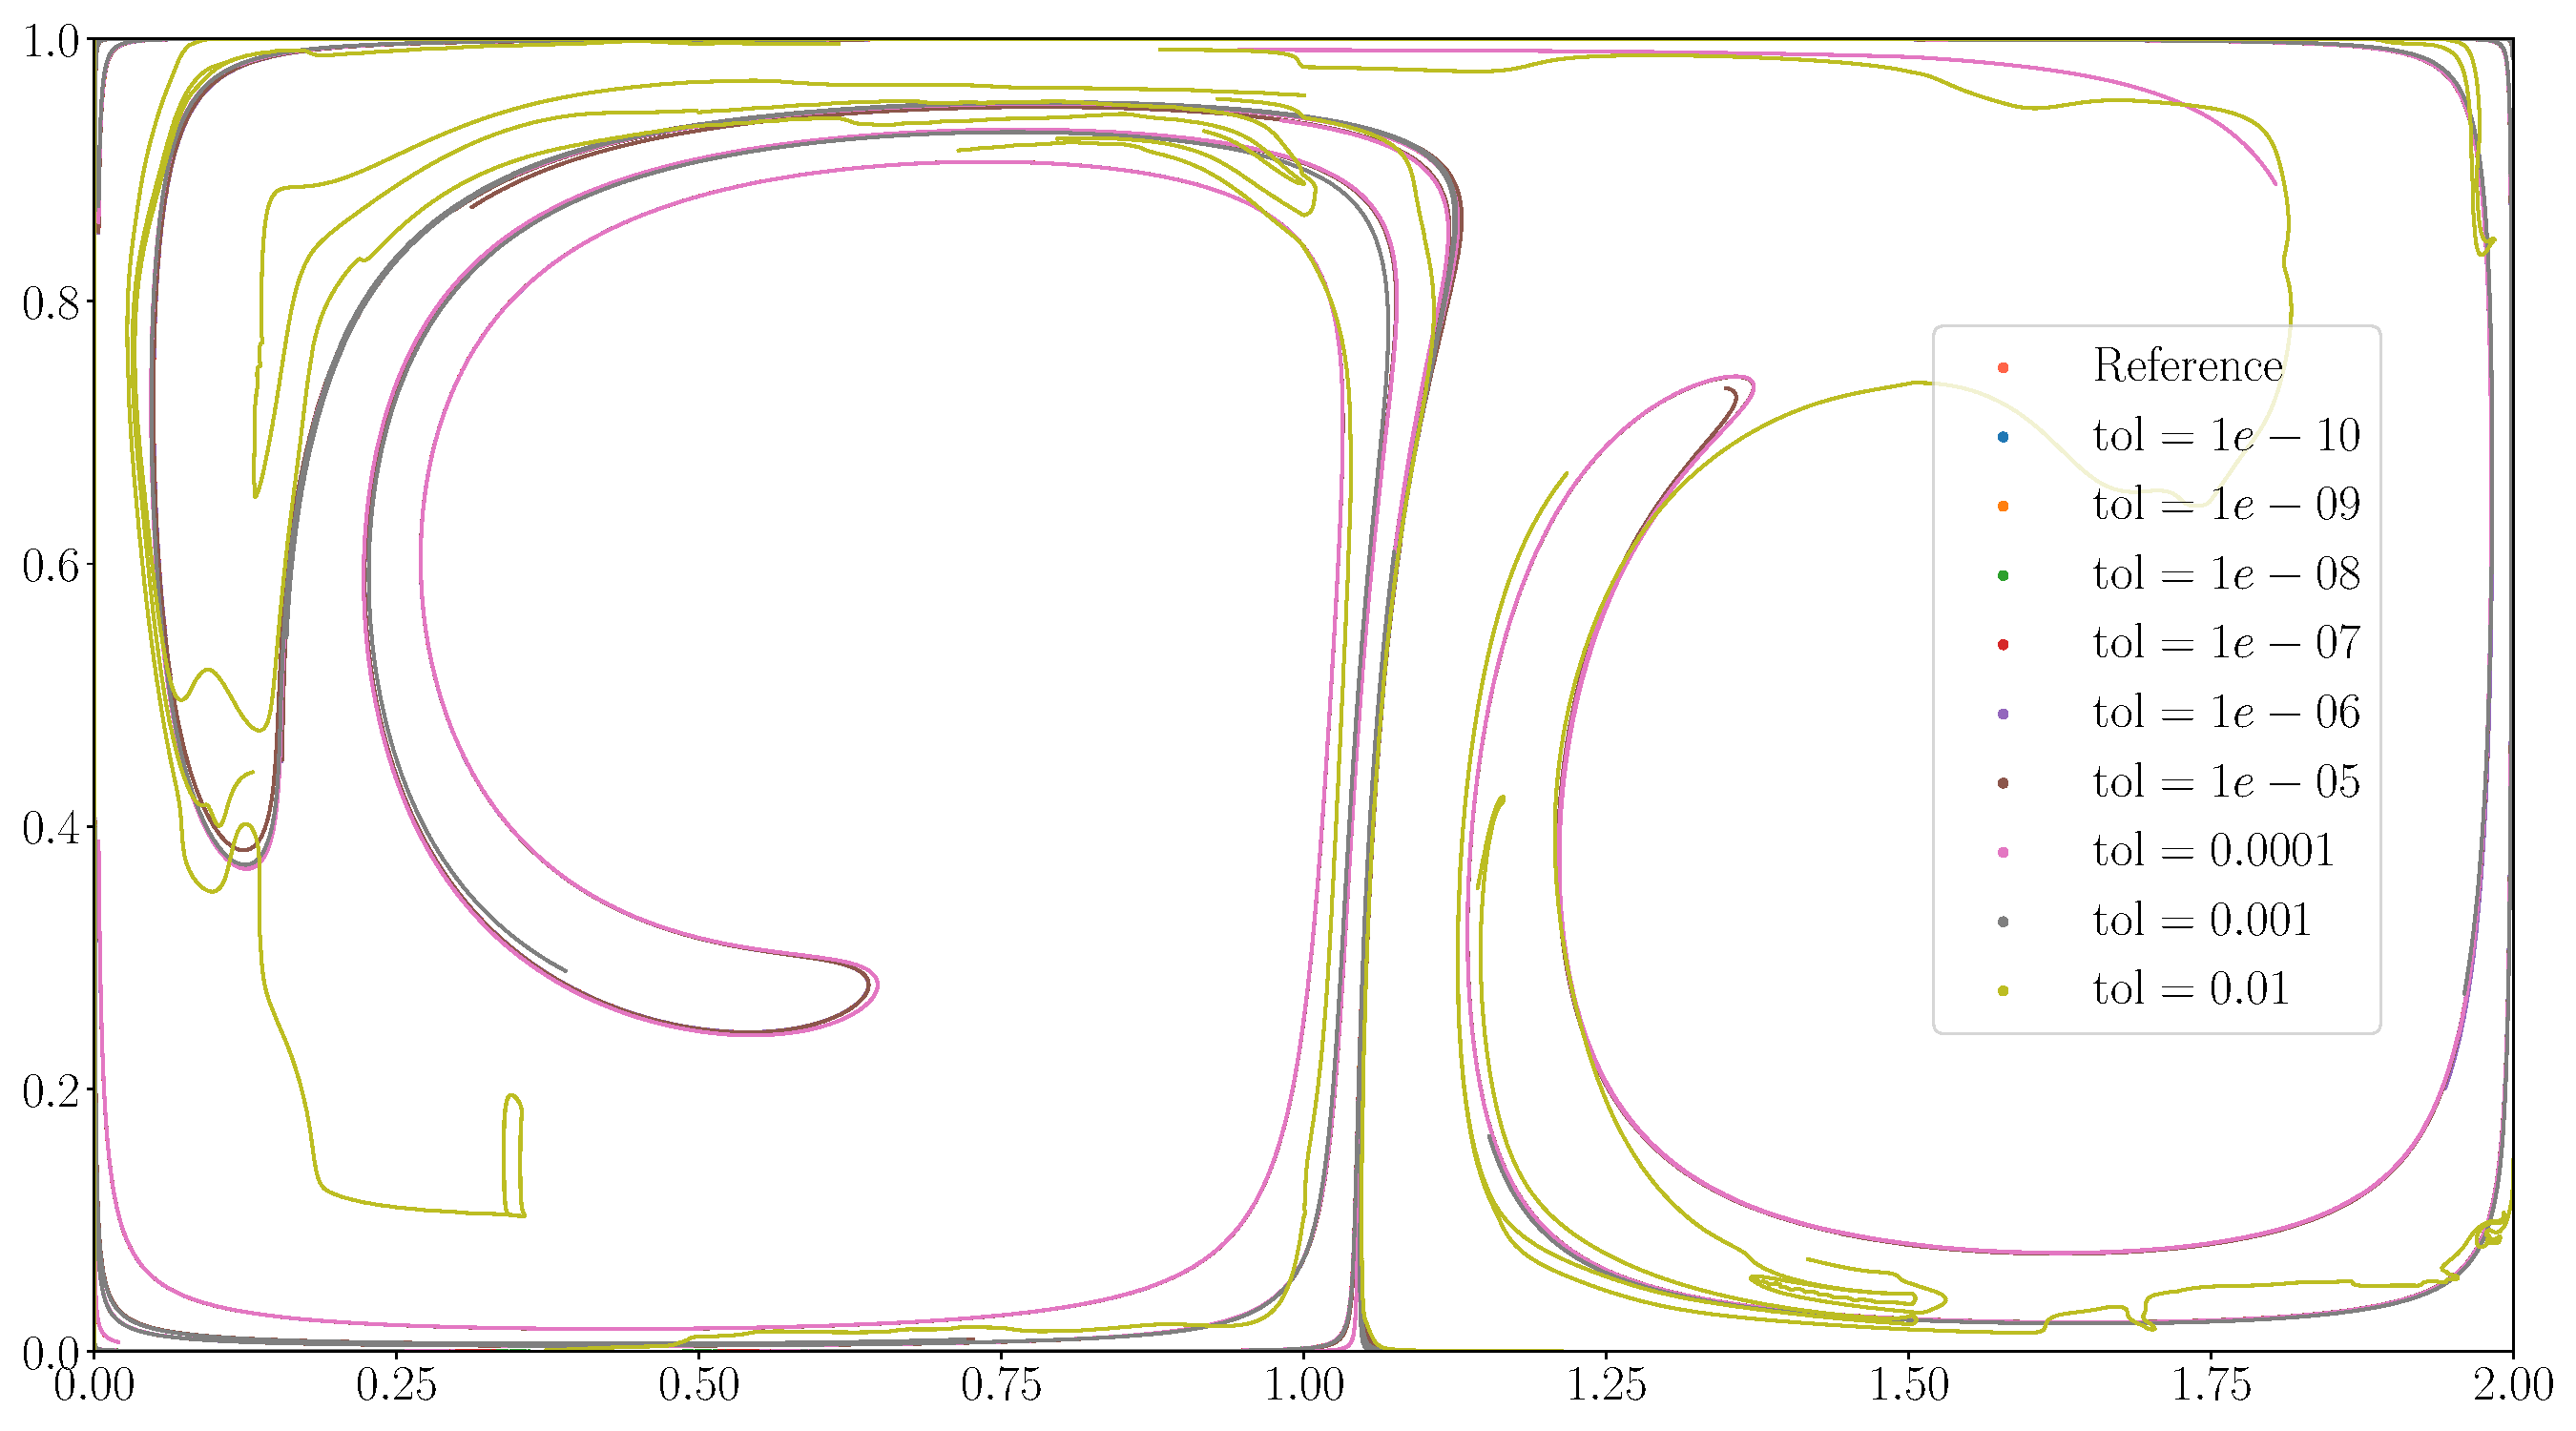
\includegraphics[width=0.9\linewidth]{figures/lcs_figures/rkdp54.pdf}
    \caption[LCS curves found by means of the Dormand-Prince 5(4) integration
    scheme]{
        LCS curves found by means of the Dormand-Prince 5(4) integration
        scheme. The reference LCS, as shown by itself in figure
        \ref{fig:referencelcs}, is plotted on the bottom layer. Note that
        the LCS for the lowest tolerance level considered, that is,
        $\textnormal{tol}=0.1$, is not included. This is because the
        corresponding $\mathcal{U}_{0}$ domain, shown in figure
        \ref{fig:u0_dp54}, and the reference $\mathcal{U}_{0}$, shown in figure
        \ref{fig:u0_domain} are dissimilar. Here, there are visible
        disparities for for all tolerance levels $\textnormal{tol}>10^{-6}$.}
    \label{fig:lcs_rkdp54}
\end{figure}


\begin{figure}[htpb]
    \centering
    \input{figures/lcs_figures/rkdp87.pgf}
    %\resizebox{0.9\linewidth}{!}{\input{figures/lcs_figures/rkdp87.pgf}}
    %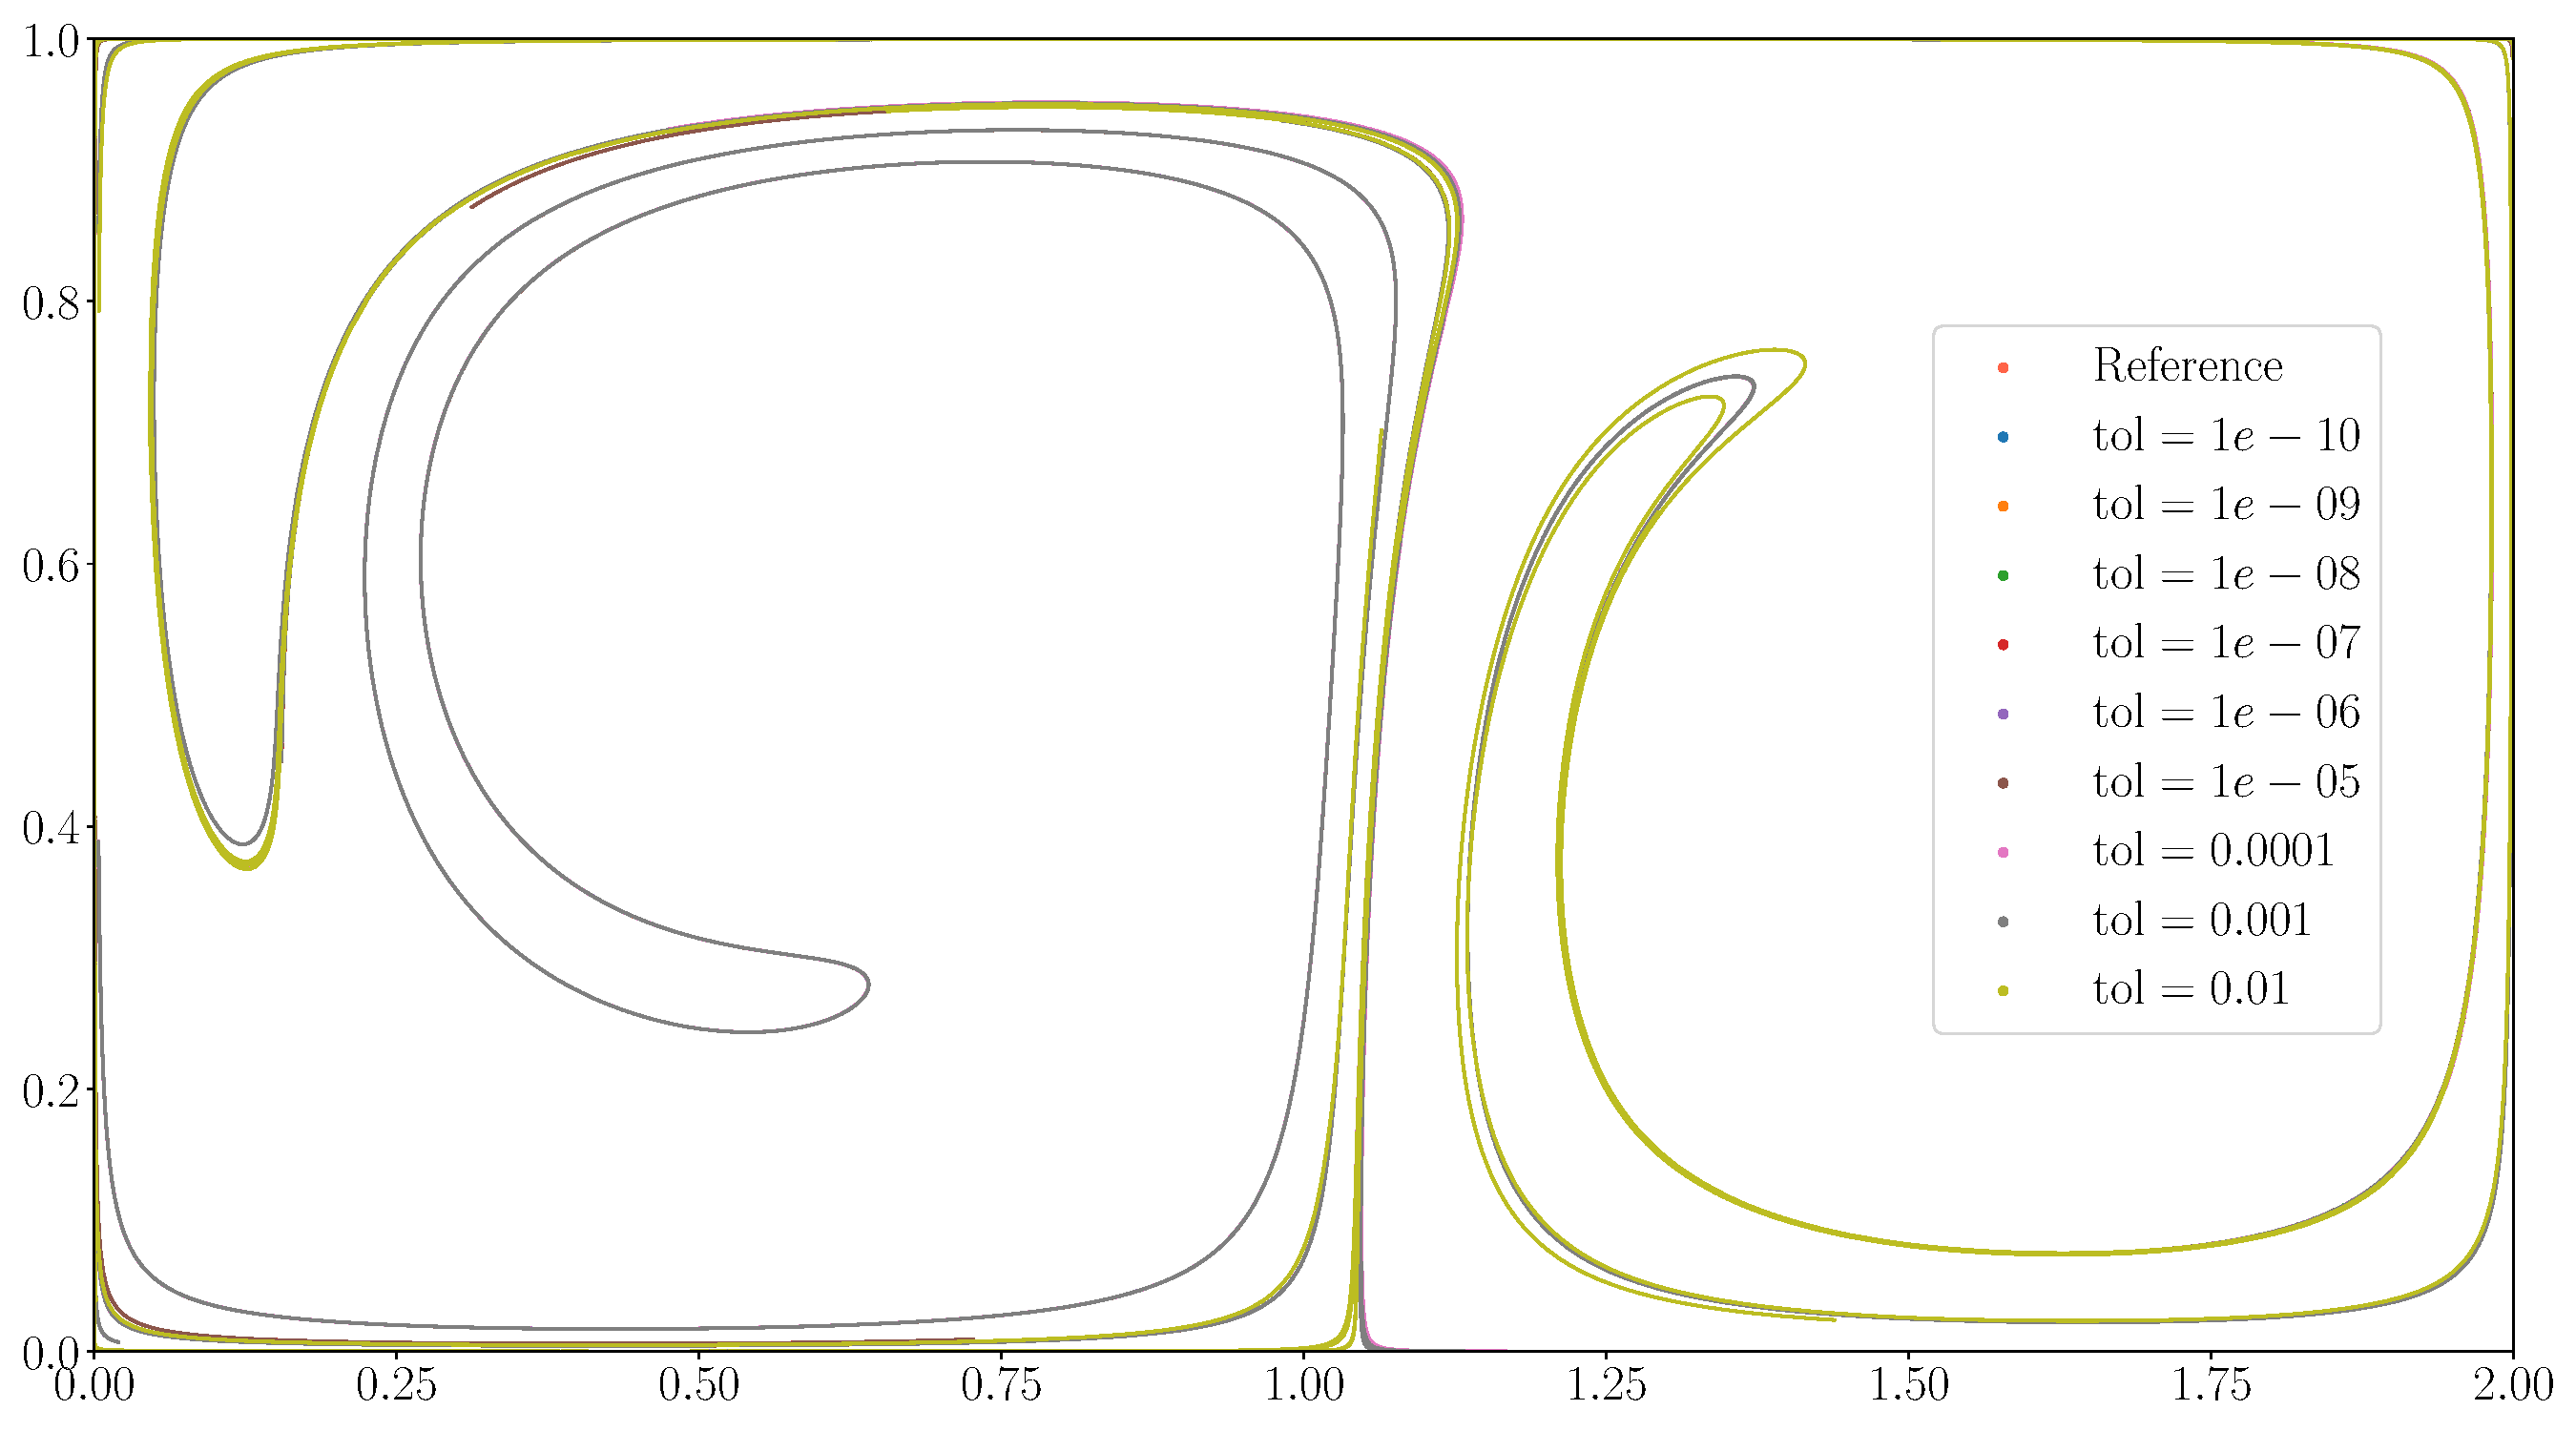
\includegraphics[width=0.9\linewidth]{figures/lcs_figures/rkdp87.pdf}
    \caption[LCS curves found by means of the Dormand-Prince 8(7) integration
    scheme]{
        LCS curves found by means of the Dormand-Prince 8(7) integration
        scheme. The reference LCS, as shown by itself in figure
        \ref{fig:referencelcs}, is dashed on the top layer. Note that
        the LCS for the lowest tolerance level considered, that is,
        $\textnormal{tol}=10^{-1}$, is not included. This is because the
        corresponding $\mathcal{U}_{0}$ domain, shown in figure
        \ref{fig:u0_dom_err_dp87}, and the reference $\mathcal{U}_{0}$, shown in figure
        \ref{fig:u0_domain} are quite unlike one another. Here, the most immediately
        discernible dissimilarities emanate from the tolerance level
    $\textnormal{tol}=10^{-2}$.}
    %Close inspection, however, reveals
    %    discrepancies for all tolerance levels $\textnormal{tol}>10^{-6}$,
    %    particularly by the `$\cap$' shape near $x=1.25$.}
    \label{fig:lcs_rkdp87}
\end{figure}





\section{Setup}
\label{sec:setup}



We consider flow in two-dimensional dynamical systems of the form


\begin{equation}
    \label{eq:odesystem}
\dot{\vct{x}} = \vct{v}(t,\vct{x}),\quad\vct{x}\in\mathcal{U},\quad{}t\in[t_{0},t_{1}],
\end{equation}

i.e., systems defined for the finite time interval $[t_{0},t_{1}]$, on an open,
bounded subset $\mathcal{U}$ of $\mathbb{R}^{2}$. In addition, the velocity
field $\vct{v}$ is assumed to be smooth in its arguments. Depending on the
exact nature of the velocity field $\vct{v}$, analytical particle trajectories,
i.e., solutions of system~\eqref{eqn:odesystem}, may or may not be computed.




\vspace{\fill}

\newpage

\chapter{Method}
\label{cha:method}
In order to investigate the dependence of LCS identification by means of
the variational approach as presented in \cref{sub:hyperbolic_lcss} on
the choice of numerical integration method, cf.\ \cref{sec:solvingsystems},
a system which has been studied extensively in the literature, was chosen.
The system, an unsteady double gyre, has been used frequently as a test case
for locating LCSs from different indicators
\parencite{farazmand2012computing,shadden2005definition}. As a result, the
LCSs the system exhibit are well known.

\section{The double gyre model}
\label{sec:the_double_gyre_model}

The double gyre model is defined as a pair of counter-rotating gyres, with a
time-periodic perturbation. The perturbation can be interpreted as a solid, as
in impenetrable, wall which oscillates periodically, which causes the gyres
to periodically contract and expand. In terms of the cartesian coordinate vector
$\vct{x}=(x,y)$, the system can be expressed mathematically as

\begin{equation}
    \label{eq:doublegyre}
    \renewcommand{\arraystretch}{2.5}
    \dot{\vct{x}} =\vct{v}(t,\vct{x})= \pi{}A\begin{pmatrix}%
        -\sin\big(\pi{}f(t,x)\big)\cos(\pi{}y)\\
        \cos\big(\pi{}f(t,x)\big)\sin(\pi{}y)\dfrac{\partial{}f(t,x)}{\partial{}x}
    \end{pmatrix}
\end{equation}

where

\begin{equation}
    \label{eq:doublegyrefuns}
    \begin{gathered}
        f(t,x) = a(t)x^{2} + b(t)x\\
        a(t) = \epsilon\sin(\omega{}t)\\
        b(t) = 1-2\epsilon\sin(\omega{}t)
    \end{gathered}
\end{equation}

and the parameters $A$, $\epsilon$ and $\omega$ dictate the nature of the
flow pattern. As in the literature, the parameter values

\begin{equation}
    \label{eq:doublegyreparams}
    \begin{gathered}
        A = 0.1\\
        \epsilon=0.1\\
        \omega=\frac{2\pi}{10}
    \end{gathered}
\end{equation}

were used \parencite{farazmand2012computing,shadden2005definition}. Moreover,
the starting time was $t_{0}=0$, and the integration time was $T=20$, i.e.,
forcing two periods of motion, cf.
\eqref{eq:doublegyreparams}.

Note that the velocity field $\vct{v}(t,\vct{x})$ in equation
\eqref{eq:doublegyre} can be expressed in terms of a scalar stream function:

\begin{equation}
    \label{eq:doublegyrestreamfun}
    \renewcommand{\arraystretch}{2.5}
    \begin{gathered}
        \psi(t,\vct{x}) = A\sin\big(\pi{}f(t,x)\big)\sin(\pi{}y) \\
        \vct{v}(t,\vct{x}) = \begin{pmatrix}%
            -\dfrac{\partial{}\psi}{\partial{}y} \\
            \dfrac{\partial{}\psi}{\partial{}x}
        \end{pmatrix}
    \end{gathered}
\end{equation}

which means that the velocity field is divergence-free by construction:

\begin{equation}
    \label{eq:doublegyreincompr}
    \vct{\nabla}\vdot\vct{v}(t,\vct{x}) = -\pdv[2]{\psi}{x}{y} %
                                        + \pdv[2]{\psi}{y}{x} = 0
\end{equation}

where the latter equality follows from Schwartz' theorem of mixed partial
derivatives, as the stream function is smooth. This means that we expect the
property given in equation~\eqref{eq:cauchygreenincomprlambda} to hold for the
double gyre flow.



\section{Advecting a set of initial conditions}
\label{sec:advecting_a_set_of_initial_conditions}

The variational model is based upon the advection of non-interacting tracers,
cf. \cref{sec:typeofflow}, by the velocity field defined in equation
\eqref{eq:doublegyre}. The system has no known analytical solution for the
tracer trajectories. Thus, it must be solved numerically, by means of some
numerical integration method, e.g.\ a Runge-Kutta method, cf.\
\cref{sub:the_runge_kutta_family_of_numerical_methods}. With the main focus
of this project being the dependence on LCSs on the chosen integration method,
the advection was performed using all of the numerical integrators introduced
in \cref{sub:the_runge_kutta_methods_under_consideration}, making use of
MPI paralellization in order to accelerate the computations.

\subsection{Generating a set of initial conditions}
\label{sub:generating_a_set_of_initial_conditions}
The computational domain $\mathcal{U}=[0\hspace{1ex}2]\times[0\hspace{1ex}1]$
was discretized by a set of linearly spaced tracers, with $1000\times500$ grid
points, effectively creating a nearly uniform grid of approximate spacing
$\Delta{x}\simeq\Delta{y}\simeq0.002$. Tracers were placed on, and within, the
domain boundaries of $\mathcal{U}$. The grid was extended artificially,
with an additional two rows or columns appended to all of the domain edges,
with the same grid spacing as the \emph{main} grid. This was done in order to
ensure that the dynamics at the domain boundaries were included in the analysis
to follow. The extended grid thus had a total of $1004\times504$ grid points.
The construction of the grid is illustrated in figure~\ref{fig:initialgrid}.

\begin{figure}[htpb]
    \centering
    \resizebox{0.8\linewidth}{!}{\input{figures/initial_grid.pdf_tex}}
    \caption[Illustration of the set of initial conditions, including
                artificial extension]{Illustration of the set of initial
                conditions, including artificial extension on all domain edges.
                Dark grey blobs signify the main grid, i.e., the tracers
                which discretize the computational domain
            $[0\hspace{1ex}2]\times[0\hspace{1ex}1]$. These were linearly
        spaced in either direction, with twice as many points in the $x$-
        direction as the $y$-direction, in order to generate an approximately
        equidistant grid, i.e., $\Delta{x}\simeq\Delta{y}$. Light grey blobs
        signify the artificially extended grid, i.e., tracers starting
        originating outside of the computational domain. These were used in
        order to properly encapsulate the dynamics at the domain boundaries,
        in the analysis to follow.}
    \label{fig:initialgrid}
\end{figure}

\subsection{On the choice of numerical step lengths and tolerance levels}
\label{sub:on_the_choice_of_numerical_step_lengths_and_tolerance_levels}

For the fixed stepsize integrators, step lengths of $10^{-1}$ through to
$10^{-5}$ were used. For a step length of $10^{-5}$, the total number of
integration steps required in order to advect the system from $t_{0}=0$ to
$t=20$ becomes $10^{6}$. Because the inherent inaccuracy of double precision
floating-point numbers is of order $10^{-16}$, the total floating point
error expected to arise when performing the integration for a step length of
$10^{-5}$ is of order $10^{-10}$. The least accurate of the fixed stepsize
integrators under consideration, the Euler method, is a \nth{1} order accurate
globally, meaning that its local error is of \nth{2} order in the time step,
cf. \cref{def:rungekuttaorder}. Thus, we expect that the local error of the
Euler method to be of order $10^{-10}$, i.e., the same order of the accumulated
floating-point errors. Reducing the time step further necessarily leads to
an increase in the accumulated floating-point errors, meaning that we cannot
reasonably expect more accurate results for the Euler method --- at the very
least, a time step of $10^{-5}$ appears to be a point after which there is
little to be gained in terms of numerical accuracy for the Euler method by
lowering the time step further. For the other fixed stepsize integrators, which
are of higher order, we expect this breaking point to occur for a (somewhat)
larger time step.

While the above logic does not translate directly for the adaptive stepsize
integrators, empirical tests indicate that for the Bogacki-Shampine integrators,
as well as the Dormand-Prince 5(4) integrator, the accumulated floating point
errors caught up to the required tolerance level at some point between the
levels $10^{-10}$ and $10^{-11}$, while the Dormand-Prince 8(7) integrator held
its ground until about $10^{-13}$. For this reason, tolerance levels of
$10^{-1}$ through to $10^{-10}$ were used for the adaptive stepsize integrators.

As previously mentioned, reference solutions must be obtained by means of a
high order fixed stepsize method with a small step length, alternatively a high
order adaptive stepsize method with a small tolerance level. In this case, the
latter approach was chosen, and the solution obtained via the Dormand-Prince
8(7) integrator with a numerical tolerance of $10^{-12}$ was used as the
reference.





\vspace{\fill}

\newpage

%\chapter{Results and Discussion}
%\label{cha:results_and_discussion}
%\section{The LCS curves obtained using the different schemes}
\label{sec:the_lcs_curves_obtained_using_the_different_schemes}

Here, the repelling LCS curves found by means of the variety of
numerical integration schemes under consideration, are presented. All of the
LCS curves obtained for a given integrator, for all numerical time step lengths
or tolerance levels are included in one figure, where the reference LCS, shown
in figure~\ref{fig:referencelcs}, is also included in order to facilitate
visual comparison. The idea is that any LCS curve that deviates from the
reference, will reveal itself by not conforming perfectly. The LCS curves
resulting from the singlestep methods are presented in
\cref{fig:lcs_euler,fig:lcs_rk2,fig:lcs_rk3,fig:lcs_rk4}, whereas the ones
found by virtue of the embedded, that is, adaptive stepsize, methods, are
shown in~\cref{fig:lcs_rkbs32,fig:lcs_rkbs54,fig:lcs_rkdp54,fig:lcs_rkdp87}.

\subsection{LCS curves stemming from singlestep methods}
\label{sub:lcs_curves_stemming_from_singlestep_methods}



\begin{figure}[htpb]
    \centering
    \input{figures/lcs_figures/euler.pgf}
    \caption[LCS curves found by means of the Euler integration scheme]{
        LCS curves found by means of the Euler integration scheme. The
        reference LCS, as shown by itself in figure~\ref{fig:referencelcs},
        is plotted on the bottom layer. There is a clearly visible offset
        compared to the reference, for all but the two smallest numerical step
        lengths considered. The two latter LCS curves appear to conform well.}
    \label{fig:lcs_euler}
\end{figure}

\begin{figure}[htpb]
    \centering
    \input{figures/lcs_figures/rk2.pgf}
    \caption[LCS curves found by means of the Heun integration scheme]{
        LCS curves found by means of the Heun integration scheme. The
        reference LCS, as shown by itself in figure~\ref{fig:referencelcs},
        is dashed on the top layer. There exists discrepancies with
        regards to the reference for the two largest numerical time step
        lengths considered. These are most prominent in the lower left corner,
        and near $x=1$.}
    \label{fig:lcs_rk2}
\end{figure}

\begin{figure}[htpb]
    \centering
    \input{figures/lcs_figures/rk3.pgf}
    \caption[LCS curves found by means of the Kutta integration scheme]{
        LCS curves found by means of the Kutta integration scheme. The
        reference LCS, as shown in figure~\ref{fig:referencelcs},
        is dashed on the top layer. There are some disparities with
        regards to the reference both for the two largest numerical
        time step lengths considered. These are most pronounced in the lower
        left corner, near the leftmost `$\cup$' shape by $y=0.4$ and the
        `$\cap$' shape near $x=1.25$.}
    \label{fig:lcs_rk3}
\end{figure}

\begin{figure}[htpb]
    \centering
    \input{figures/lcs_figures/rk4.pgf}
    \caption[LCS curves found by means of the classical Runge-Kutta integration scheme]{
        LCS curves found by means of the classical Runge-Kutta integration scheme. The
        reference LCS, as shown by itself in figure~\ref{fig:referencelcs},
        is dashed on the top layer. One of the very few visible
        discrepancies belongs to the second largest numerical time step length
        considered, and is located in the lower left corner.}
    \label{fig:lcs_rk4}
\end{figure}


The LCS curves obtained from the Euler scheme using relatively large step
lengths are the most obviously incorrect ones, in comparison to the reference.
There appears to be very little separating the performance of the other
singlestep methods. Interestingly, the Heun scheme appears to yield more
accurate results than the Kutta scheme for all the considered step lengths.
This is somewhat unexpected, because, as mentioned in
\cref{sub:the_runge_kutta_methods_under_consideration}, the Heun scheme is
\nth{2}-order accurate in the time step, whereas the Kutta scheme is
\nth{3}-order accurate. On a less surprising note, seeing as it is \nth{4}-order
accurate, the classical Runge-Kutta scheme produces very accurate curves for
all step lengths.

\subsection{LCS curves stemming from adaptive stepsize methods}
\label{sub:lcs_curves_stemming_from_adaptive_stepsize_methods}

Note that, although numerical tolerance levels of $10^{-1}$ through to
$10^{-10}$ were investigated, the figures presented here do not show LCS curves
for $\textnormal{tol}=10^{-1}$. This is due to the fact that, for all
embedded methods, none of the resulting domains $\mathcal{U}_{0}$ bore
a great amount of resemblance to the reference. This resulted in very disparate
behaviour of strainlines, to the extent that the resulting strain systems were
too dissimilar to the reference to warrant any meaningful comparisons. The
erroneous $\mathcal{U}_{0}$ domains are shown in~\cref{fig:u0_dom_errs}
(compare to~\cref{fig:u0_domain}).
%In fact, most likely because of the large density of points in these domains,
%keeping track of the neighbors for each individual strainline and its
%intersections with the lines in $\mathcal{L}$ turned out to be an unconquerable
%task. It is known that storing the necessary data requires in excess of 28 GB
%of memory, at which point even the NTNU supercomputer, Vilje, proved
%insufficient.

Notably, all of the embedded integration methods result in LCSs which are
dissimilar from the reference for the tolerance level $\textnormal{tol}=10^{-2}$,
where only the curve obtained by the Dormand-Prince 8(7) scheme is anything
alike the reference. More curiously, the Bogacki-Shampine 3(2) method appears
to outperform its theoretically more accurate sibling --- the
Bogacki-Shampine 5(4) method --- even for relatively
large tolerance levels. This is visible in the
vicinity of the `$\cup$' shape near $y=0.4$ in~\cref{fig:lcs_rkbs32,fig:lcs_rkbs54},
for instance. Furthermore, the Dormand-Prince 5(4) method appears to yield more
accurate LCS curves in general, than the Bogacki-Shampine 5(4) method. This
is somewhat surprising, given that the latter scheme is supposedly more accurate
than other methods of similar order, as mentioned in
\cref{sub:the_runge_kutta_methods_under_consideration}. Lastly, the
Dormand-Prince 8(7) method appears to produce very accurate results for all
tolerance levels smaller than $10^{-2}$, and, as previously mentioned, gives
the most correct LCS curve for the tolerance level $10^{-2}$
--- which is to be expected, as it is the highest order method among the ones
considered, after all.
\vspace{\fill}

\begin{figure}[htpb]
    \centering
    \begin{subfigure}[b]{0.475\textwidth}
        \centering
        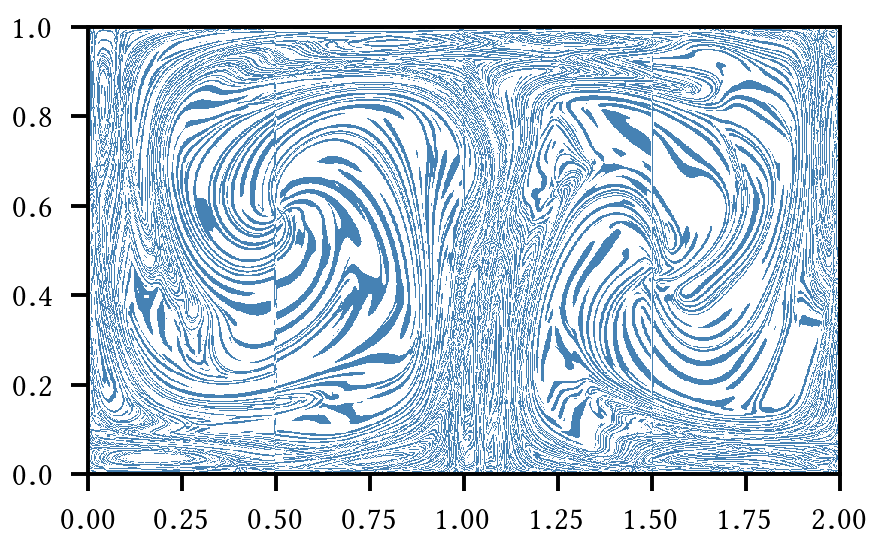
\includegraphics{figures/domain_figures/rkbs32_err_half_width.png}
        \caption[]{{\small Bogacki-Shampine 3(2)}}
        \label{fig:u0_dom_err_bs32}
    \end{subfigure}
    \begin{subfigure}[b]{0.475\textwidth}
        \centering
        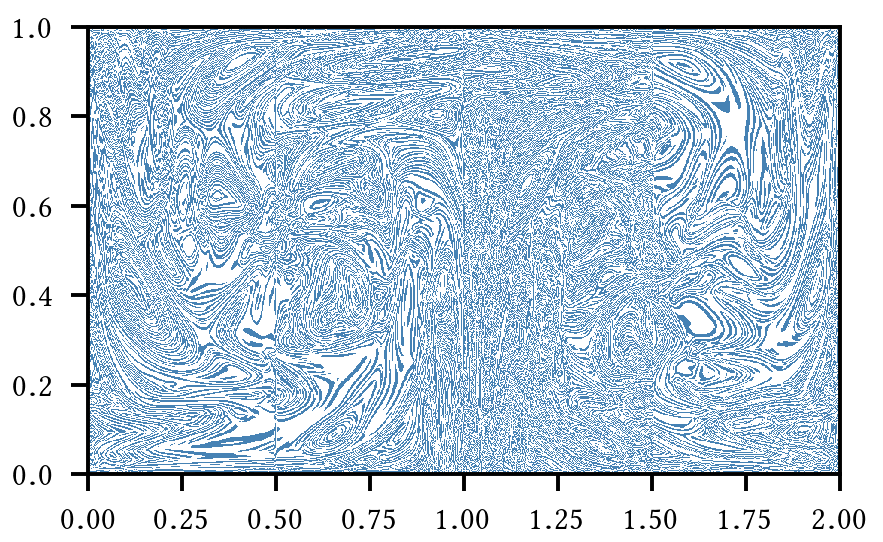
\includegraphics{figures/domain_figures/rkbs54_err_half_width.png}
        \caption[]{{\small Bogacki-Shampine 5(4)}}
        \label{fig:u0_dom_err_bs54}
    \end{subfigure}

    \begin{subfigure}[b]{0.475\textwidth}
        \centering
        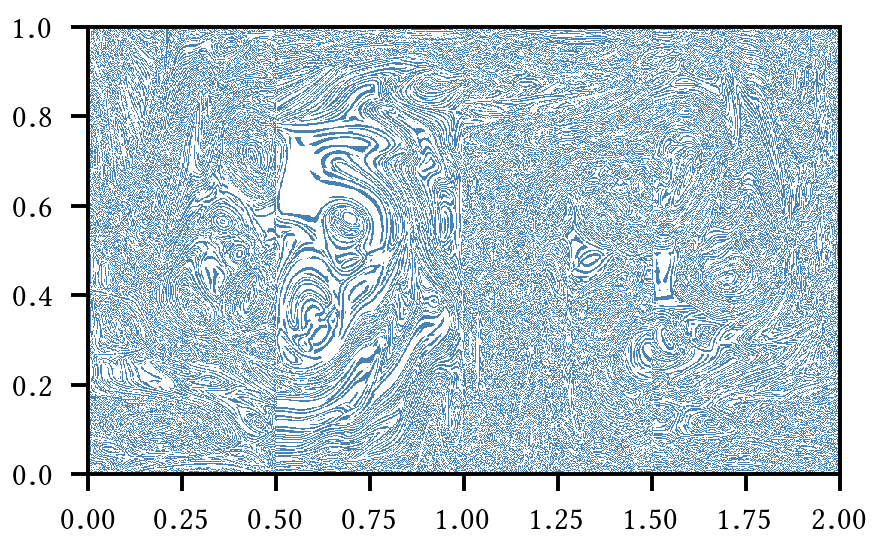
\includegraphics{figures/domain_figures/rkdp54_err_half_width.png}
        \caption[]{{\small Dormand-Prince 5(4)}}
        \label{fig:u0_dom_err_dp54}
    \end{subfigure}
    \begin{subfigure}[b]{0.475\textwidth}
        \centering
        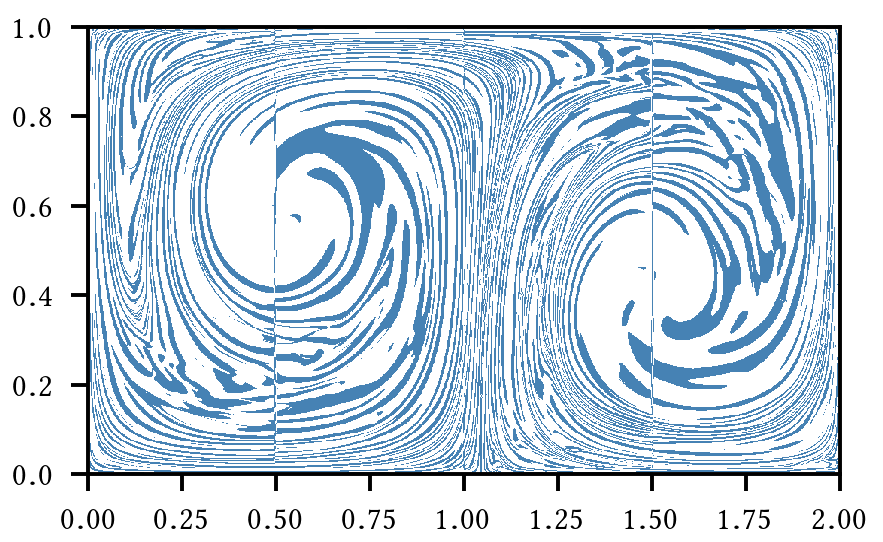
\includegraphics{figures/domain_figures/rkdp87_err_half_width.png}
        \caption[]{{\small Dormand-Prince 8(7)}}
        \label{fig:u0_dom_err_dp87}
    \end{subfigure}
    \caption[The $\mathcal{U}_{0}$ domains obtained with the adaptive stepsize
    integration schemes, with numerical tolerance level
    $\textnormal{tol}=10^{-1}$]{
        The $\mathcal{U}_{0}$ domains obtained with the adaptive stepsize
        integration schemes, with numerical tolerance level
        $\textnormal{tol}=10^{-1}$. Out of the four schemes considered, only the
    Dormand-Prince 8(7) method is remotely close to reproducing the
    reference domain, shown in~\ref{fig:u0_domain}. In any case, the
    differences are sufficiently large to alter the resulting strain
    system beyond recognition, rendering LCS comparisons with the reference
    impractical.}
    \label{fig:u0_dom_errs}
\end{figure}



\begin{table}[htpb]
    \centering
    \caption[Butcher tableau representation of the Bogacki-Shampine 3(2)
    embedded Runge-Kutta method]{Butcher tableau representation of the Bogacki-
    Shampine 3(2) embedded Runge-Kutta method. The $b$ coefficients correspond
to a \nth{3}-order accurate solution used to continue the integration. The
$\widehat{b}$ coefficients correspond to a \nth{2}-order accurate interpolant,
which can be used to estimate the error of the numerical approximation, and to
dynamically adjust the time step. The \emph{First Same As Last} property is
apparent from the fact that the $b$ coefficients correspond exactly to the
last row of coefficients in the Runge-Kutta matrix. For reference, see
\textcite{bogacki1989pair}.}
    \label{tab:butcherbs32}
    \renewcommand{\arraystretch}{2.5}
    \begin{tabular}{C|CCCC}
        \toprule
        0 & \\
        \dfrac{1}{2} & \dfrac{1}{2} \\
        \dfrac{3}{4} & 0 & \dfrac{3}{4} \\
        1 & \dfrac{2}{9} & \dfrac{1}{3} & \dfrac{4}{9} \\
        \hline
        & \dfrac{2}{9} & \dfrac{1}{3} & \dfrac{4}{9} \\
        \hline
        & \dfrac{7}{24} & \dfrac{1}{4} & \dfrac{1}{3} & \dfrac{1}{8} \\
        \bottomrule
    \end{tabular}
\end{table}

%\clearpage
\begin{table}[htpb]
\centering
    \caption[Butcher tableau representation of the Bogacki-Shampine 5(4)
    embedded Runge-Kutta method]{Butcher tableau representation of the Bogacki-
    Shampine 5(4) embedded Runge-Kutta method. The $b$ coefficients correspond
to a \nth{5} order accurate solution used to continue the integration. The
two rows of $\widehat{b}$ coefficients correspond to two independent \nth{4}
order accurate interpolants. They can be used to estimate the error of the
numerical approximation, and to dynamically adjust the time step. The fact that
two independent interpolants are included is a part of the reason for which
the method nearly behaves like a \nth{6} order method
\parencite[p.194 in the 2008 printing]{hairer1993solving}. The
\emph{First Same As Last} property is apparent from the fact that the $b$
coefficients correspond exactly to the last row of coefficients in the
Runge-Kutta matrix. For reference, see~\textcite{bogacki1996efficient}.}
    \label{tab:butcherbs54}
    \renewcommand{\arraystretch}{2.5}
    \begin{tabular}{C|CCCCCCCC}
        \toprule
        0 & \\
        \dfrac{1}{6} & \dfrac{1}{6} \\
        \dfrac{2}{9} & 0 & \dfrac{2}{27} & \dfrac{4}{27} \\
        \dfrac{3}{7} & \dfrac{183}{1372} & \dfrac{-162}{343} %
                     & \dfrac{1053}{1372} \\
        \dfrac{2}{3} & \dfrac{68}{297} & \dfrac{-4}{11} & \dfrac{42}{143} %
                     & \dfrac{1960}{3861} \\
        \dfrac{3}{4} & \dfrac{597}{22528} & \dfrac{81}{352} %
                     & \dfrac{63099}{585728} & \dfrac{58653}{366080} %
                     & \dfrac{4617}{20480} \\
        1 & \dfrac{174197}{959244} & \dfrac{-30942}{79937} %
          & \dfrac{8152137}{19744439} & \dfrac{666106}{1039181} %
          & \dfrac{-29421}{29068} & \dfrac{482048}{414219} \\
        1 & \dfrac{587}{8064} & 0 & \dfrac{4440339}{15491840} %
          & \dfrac{24353}{124800} & \dfrac{387}{44800} & \dfrac{2152}{5985} %
          & \dfrac{7267}{94080} \\
        \hline
          & \dfrac{587}{8064} & 0 & \dfrac{4440339}{15491840} %
          & \dfrac{24353}{124800} & \dfrac{387}{44800} & \dfrac{2152}{5985} %
          & \dfrac{7267}{94080} \\
        \hline
        & \dfrac{6059}{80640} & 0 & \dfrac{8559189}{30983680} %
        & \dfrac{26411}{124800} & \dfrac{-927}{89600} & \dfrac{443}{1197} %
                              & \dfrac{7267}{94080} \\
        & \dfrac{2479}{34992} & 0 & \dfrac{123}{416} & \dfrac{612941}{3411720} %
        & \dfrac{43}{1440} & \dfrac{2272}{6561} & \dfrac{79937}{1113912} %
        & \dfrac{3293}{556956} \\
        \bottomrule
    \end{tabular}
\end{table}

\begin{figure}[htpb]
    \centering
    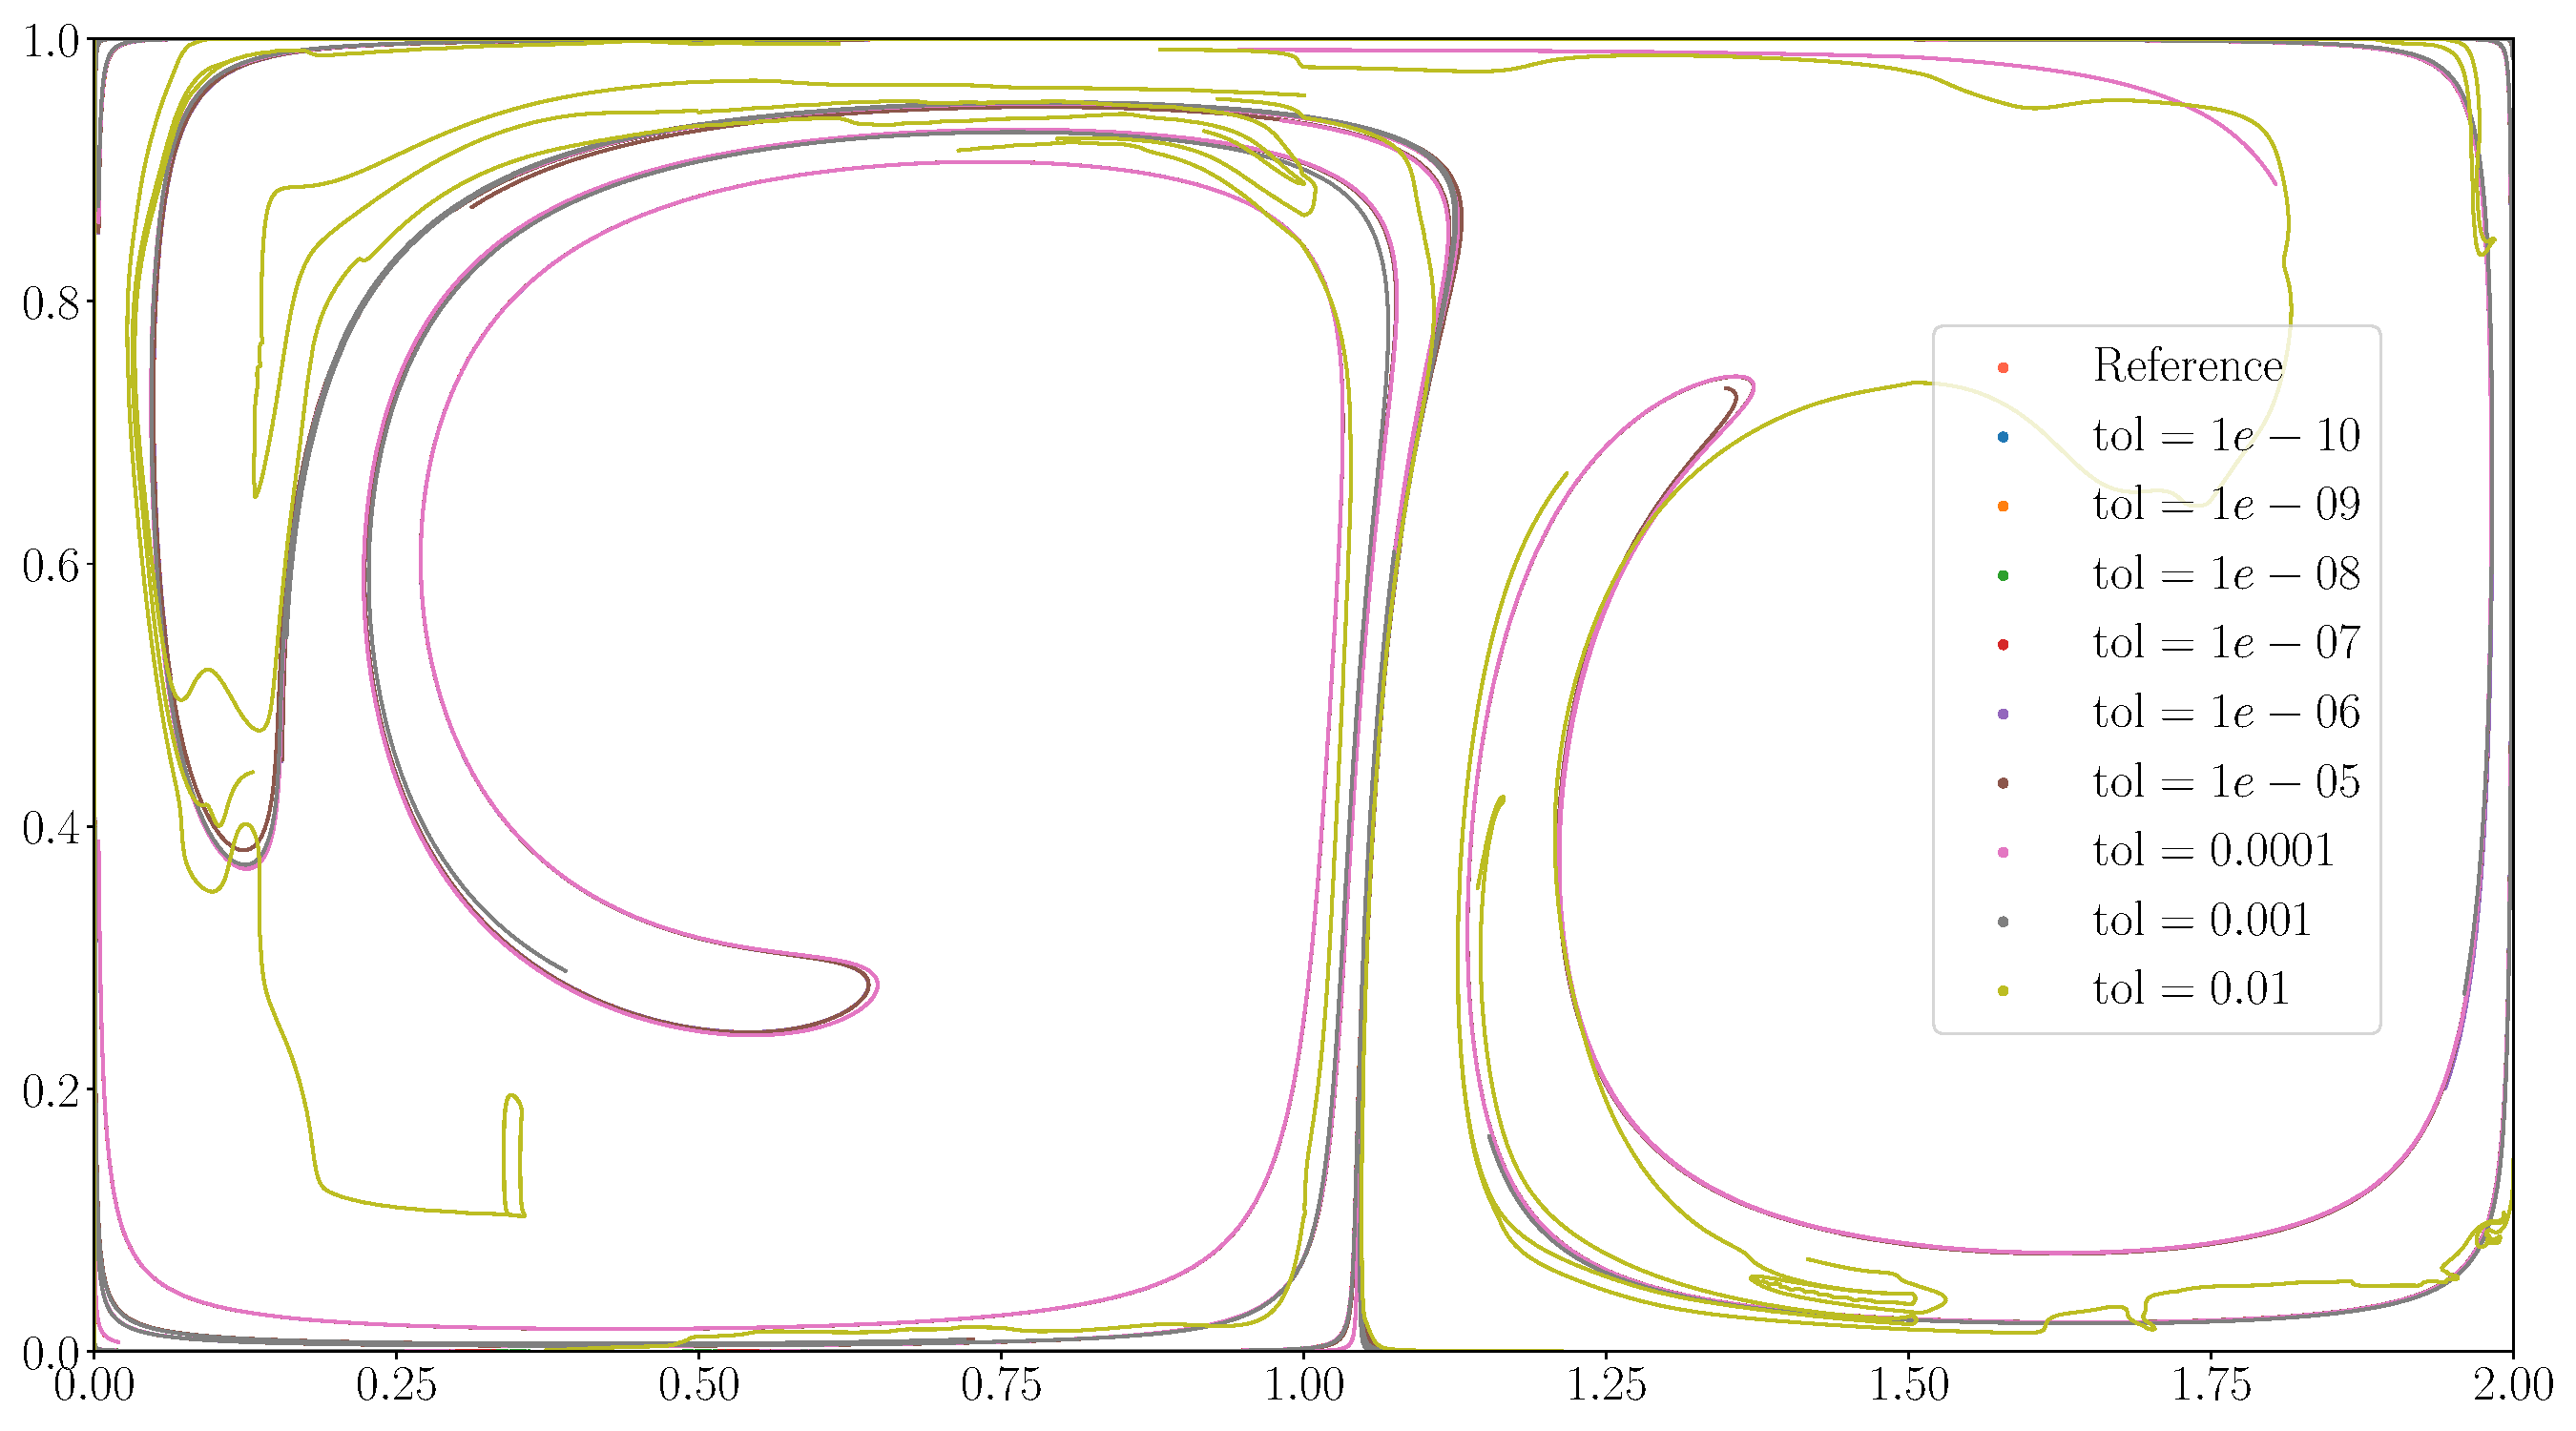
\includegraphics[width=0.9\linewidth]{figures/lcs_figures/rkdp54.pdf}
    \caption[LCS curves found by means of the Dormand-Prince 5(4) integration
    scheme]{
        LCS curves found by means of the Dormand-Prince 5(4) integration
        scheme. The reference LCS, as shown by itself in figure
        \ref{fig:referencelcs}, is plotted on the bottom layer. Note that
        the LCS for the lowest tolerance level considered, that is,
        $\textnormal{tol}=0.1$, is not included. This is because the
        corresponding $\mathcal{U}_{0}$ domain, shown in figure
        \ref{fig:u0_dp54}, and the reference $\mathcal{U}_{0}$, shown in figure
        \ref{fig:u0_domain} are dissimilar. Here, there are visible
        disparities for for all tolerance levels $\textnormal{tol}>10^{-6}$.}
    \label{fig:lcs_rkdp54}
\end{figure}


\begin{figure}[htpb]
    \centering
    \input{figures/lcs_figures/rkdp87.pgf}
    %\resizebox{0.9\linewidth}{!}{\input{figures/lcs_figures/rkdp87.pgf}}
    %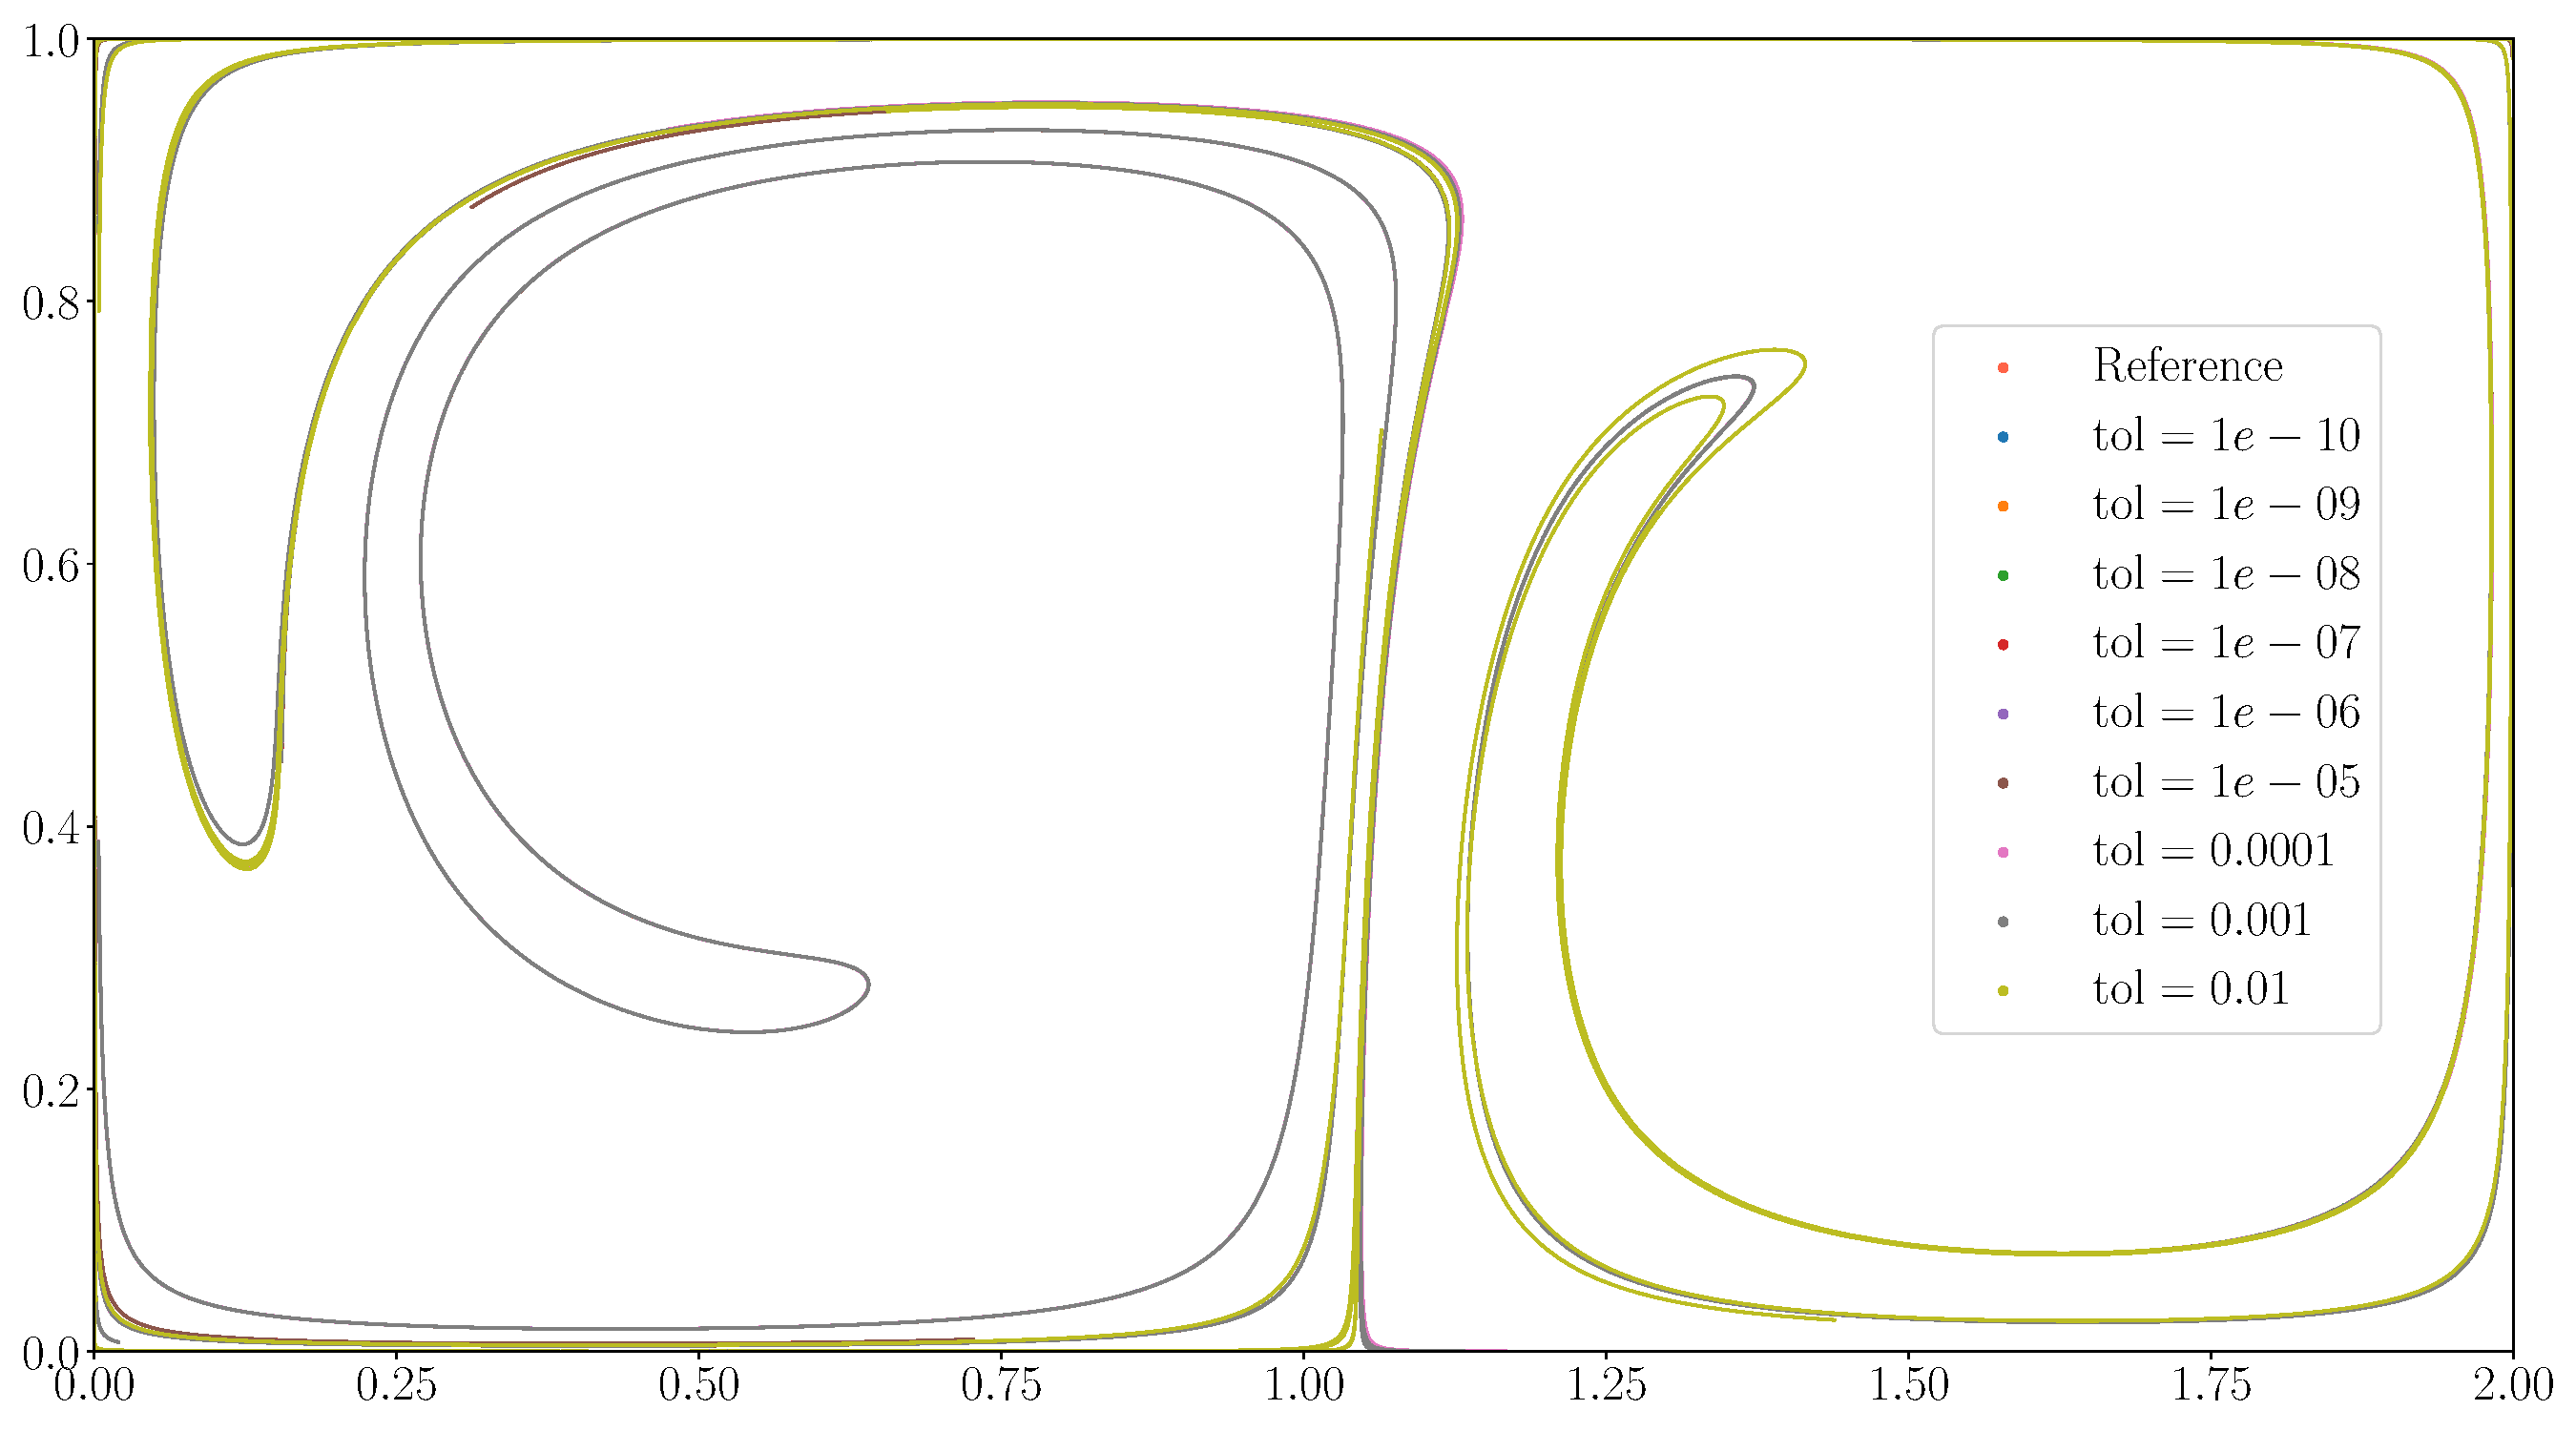
\includegraphics[width=0.9\linewidth]{figures/lcs_figures/rkdp87.pdf}
    \caption[LCS curves found by means of the Dormand-Prince 8(7) integration
    scheme]{
        LCS curves found by means of the Dormand-Prince 8(7) integration
        scheme. The reference LCS, as shown by itself in figure
        \ref{fig:referencelcs}, is dashed on the top layer. Note that
        the LCS for the lowest tolerance level considered, that is,
        $\textnormal{tol}=10^{-1}$, is not included. This is because the
        corresponding $\mathcal{U}_{0}$ domain, shown in figure
        \ref{fig:u0_dom_err_dp87}, and the reference $\mathcal{U}_{0}$, shown in figure
        \ref{fig:u0_domain} are quite unlike one another. Here, the most immediately
        discernible dissimilarities emanate from the tolerance level
    $\textnormal{tol}=10^{-2}$.}
    %Close inspection, however, reveals
    %    discrepancies for all tolerance levels $\textnormal{tol}>10^{-6}$,
    %    particularly by the `$\cap$' shape near $x=1.25$.}
    \label{fig:lcs_rkdp87}
\end{figure}





\section{Measures of error}
\label{sec:measures_of_error}

Here, the measures of error introduced in~\cref{sec:estimation_of_errors} for
the different numerical integration schemes considered, are presented. For
each different type of error, two figures are included. One in which the error
of the singlestep methods is shown as a function of the integration step length,
and one in which the error of \emph{all} the integration methods is shown
as a function of the number of times right hand side of the ordinary
differential equation system, that is, the velocity field given by
\cref{eq:doublegyre}, was evaluated for each step length or tolerance level.
The reason for which only the singlestep errors are included in the first set of
figures, is that they are the only methods where the error is expected to scale
as a power law in $h$, per \cref{def:rungekuttaorder}. This is naturally not the
case for the adaptive stepsize methods, where the step length varies.

More pertinent information can be found in the second set of figures, where
a well-suited integration method is characterized by generating small
errors at a small cost in terms of the required number of function calls,
in this case, the number of times the velocity field had to be evaluated.
Unlike the singlestep integrators, the advection of each tracer by means
of an adaptive stepsize method in principle requires a different number of
integration steps, and thus function evaluations. Thus, the presented number of
function evaluations is the \emph{average} across all of the advected tracers,
including the number of evaluations associated with rejected trial integration
steps. The number of function evaluations for each step of the considered
Runge-Kutta methods can be found as the number of rows in the Runge-Kutta
matrices of
\cref{tab:butchereuler,tab:butcherrk2,tab:butcherrk3,tab:butcherrk4,%
tab:butcherbs32,tab:butcherbs54,tab:butcherdopri54,tab:butcherdopri87}.
\subsection{Computed deviations in the flow maps}
\label{sub:computed_deviations_in_the_flow_maps}


Figure~\ref{fig:flowmap_err_fixed} indicates that the $\rmsd$ of the flow maps,
as defined in equation~\eqref{eq:rmsdflowmap} follow the expected power laws
of the numerical errors for the various singlestep integrators. This is
as expected, because the flow maps are found by direct application of the
numerical integrators. Furthermore, the flow map $\rmsd$ seem to exhibit
boundedness from below by the counteracting accumulated floating-point
arithmetic error, as hypothesized in
\cref{sub:on_the_choice_of_numerical_step_lengths_and_tolerance_levels}.
This effect is most prominent in the error curves of the Kutta and
classical Runge-Kutta schemes, which inflect upwards for sufficiently small
step lengths. Figure~\ref{fig:flowmap_err_both} indicates that this effect
did not materialize for the adaptive stepsize methods, for the considered
numerical tolerance levels.

Figure~\ref{fig:flowmap_err_both} reveals that the Bogacki-Shampine 3(2) scheme
is the `cheapest' in terms of the required number of function evaluations when
only a very crude approximation is needed, that is, using a very high
numerical tolerance level. Furthermore, the its higher order sibling is able
to keep up with the Dormand-Prince 8(7) method regarding efficiency, until
a mean of approximately $600$ function evaluations. This complies with the
notion that the Bogacki-Shampine 5(4) method is highly optimized and practically
behaves as an even higher order order method, as mentioned in
\cref{sub:the_runge_kutta_methods_under_consideration}.
Interestingly, there does not seem to be a direct correspondence between the
$\rmsd$ of the flow maps, and that of the computed LCS curves, presented in
\cref{sub:computed_deviations_in_the_lcs_curves}.

\input{mainmatter/results/figures/error_figures/flowmap_error_fixed_steplength.tex}

\input{mainmatter/results/figures/error_figures/flowmap_error_both.tex}

\subsection{Computed deviations in the strain eigenvalues and -vectors}
\label{sub:computed_deviations_in_the_strain_eigenvalues_and_vectors}

For brevity, only the $\rmsd$ of $\lambda_{2}$ and the direction of
$\vct{\xi}_{2}$, are included here. The latter is justified because of
the orthogonality of the eigenvectors of the Cauchy-Green strain tensor, which
means that the $\rmsd$ of the directions of both eigenvectors \emph{must} be
identical. Furthermore, the $\rmsd$ of $\lambda_{1}$ scales similarly to
that of $\lambda_{2}$, both as a function of numerical step length (for the
singlestep methods) and the number of function evaluations. Additionally, the
numerical reformulation of the existence theorem for hyperbolic LCSs, given in
\cref{eq:numericalexistence}, exhibits a more sensitive dependence to
$\lambda_{2}$ than $\lambda_{1}$. This is explicitly observable from
conditions~\eqref{eq:numericalexistence2} and~\eqref{eq:numericalexistence4},
and favors $\lambda_{2}$ as the most crucial eigenvalue.

Figure~\ref{fig:lmbd2_err_fixed} indicates that the $\rmsd$ of $\lambda_{2}$,
as defined in~\cref{eq:rmsdlmbd}, follows the anticipated scalings with the
step lengths for the various singlestep integrators. Interestingly, the $\rmsd$
dependence on the numerical step length is completely analogous to that of the
$\rmsd$ of the flow maps, as presented in
\cref{sub:computed_deviations_in_the_flow_maps}. Furthermore, inspection of
figure~\ref{fig:lmbd2_err_both} reveals that the $\rmsd$ of the $\lambda_{2}$
scales similarly to the $\rmsd$ of the flow maps for all of the integration
schemes, differing only by a numerical prefactor. This makes sense, seeing as
the calculation of the Cauchy-Green strain tensor field is based upon
finite differencing applied to the flow map, as described in
\cref{sec:calculating_the_cauchy_green_strain_tensor}.

\input{mainmatter/results/figures/error_figures/lmbd2_error_fixed_steplength.tex}

\input{mainmatter/results/figures/error_figures/lmbd2_error_both.tex}

\vspace{\fill}
\newpage

\Cref{fig:xi2_err_fixed} reveals that the $\rmsd$ of the eigenvector direction,
as defined in~\cref{eq:rmsddirection}, follows the anticipated scalings with
the step lengths for the various singlestep integrators to some degree. The
$\rmsd$ dependence on the numerical step length is not entirely analogous to
that of the $\rmsd$ of $\lambda_{2}$. Notably, the error in the eigenvector
directions is two to three orders of magnitude smaller than the error
in $\lambda_{2}$, for any given step size. This can be understood as a
consequence of using the auxiliary tracers in order to compute the strain
eigenvectors, as described in
\cref{sec:calculating_the_cauchy_green_strain_tensor}, which, by construction,
is more accurate than using the main tracers (which are used to
compute the strain eigenvalues). \Cref{fig:xi2_err_both} shows that the $\rmsd$ of
the eigenvector direction behaves qualitatively like that of the
$\rmsd$ of $\lambda_{2}$ (see~\cref{fig:lmbd2_err_both}) as a function
of the required number of function evaluations for each integration scheme.
Like for the singlestep methods, the $\rmsd$ of the eigenvector direction for
the embedded methods is generally between two and three orders of magnitude
smaller than the $\rmsd$ of $\lambda_{2}$ for any given number of function
evaluations.

%Figure~\ref{fig:xi2_err_fixed} reveals that the $\rmsd$ of the eigenvector
%direction, as defined in~\cref{eq:rmsddirection}, is negligible for
%all numerical step lengths. In fact, the numerical errors are comparable
%to, or even smaller than, the machine epsilon of double-precision floating-point
%numbers, which, as mentioned in
%\cref{sub:generating_a_set_of_initial_conditions}, is of order $10^{-16}$
%\parencite{ieee2008standard}. Because these errors are so small, the agreement
%with the anticipated scalings with the stepsize should not necessarily be taken
%as conclusive evidence of general behaviour. Figure~\ref{fig:xi2_err_both},
%shows that this is in fact the case for the adaptive stepsize methods too,
%aside from the tolerance level $\textnormal{tol}=10^{-1}$, which corresponds to
%the fewest function evaluations for each scheme. As has already been
%established in figure \ref{fig:u0_dom_errs}, for that tolerance level, none of
%the integrators yield $\mathcal{U}_{0}$ domains with reasonable degrees of
%resemblance to the reference, which is shown in figure~\ref{fig:u0_domain}.
%
From \cref{fig:lmbd2_err_both,fig:xi2_err_both}, it is clear that the
$\rmsd$s of $\lambda_{2}$ and the eigenvector direction are both quite large
for the tolerance level $\textnormal{tol}=10^{-1}$ (corresponding to the
smallest number of function evaluations) for all of the embedded methods.
This seems reasonable, given the erroneous $\mathcal{U}_{0}$ domains
obtained for that tolerance level, shown in~\cref{fig:u0_dom_errs} (compare
to~\cref{fig:u0_domain}). Moreover, the sharp turns which are present in
some of the computed LCS curves, perhaps most prominently in
\cref{fig:lcs_rkbs54,fig:lcs_rkdp54} for the tolerance level
$\textnormal{tol}=10^{-2}$, are likely a consequence of the error in the
eigenvalues and -vectors being sufficient for the corresponding
$\mathcal{U}_{0}$ domains to extend to regions in which there are very
strong local orientational discontinuities in the $\vct{\xi}_{1}$-field.
There, the special-purpose linear interpolation introduced in
\cref{sub:a_framework_for_computing_smooth_strainlines} is evidently
insufficient for computing smooth strainlines.

%Aside from the least accurate tolerance level for the embedded integrators,
%though, the error in eigenvector direction is comparable to, or smaller than,
%double-precision machine epsilon. Thus, we may conclude that the eigenvector
%directions are computed correctly for just about any tolerance level and
%numerical time step length. This can be understood as a consequence of the use
%of the auxiliary tracers in order to compute the strain eigenvectors, as
%described in~\cref{sec:calculating_the_cauchy_green_strain_tensor}, which, by
%construction, is more accurate than using the main tracers. Moreover, these
%results imply that the error in the resulting LCS curves are strongly driven by
%the error in the computed eigenvalues. The sharp turns in the computed LCS
%curves for the tolerance level $10^{-2}$, which are particularly visible
%in~\cref{fig:lcs_rkbs54,fig:lcs_rkdp54}, are likely a consequence of the
%corresponding $\mathcal{U}_{0}$ domains extending to regions in which
%there are very strong local orientational discontinuities in the
%$\vct{\xi}_{1}$-field, for which the special-purpose linear interpolation
%introduced in~\cref{sub:a_framework_for_computing_smooth_strainlines} is
%evidently insufficient.
%
\input{mainmatter/results/figures/error_figures/xi2_error_fixed_steplength.tex}


\input{mainmatter/results/figures/error_figures/xi2_error_both.tex}

%\clearpage

\subsection{Computed deviations in the LCS curves}
\label{sub:computed_deviations_in_the_lcs_curves}

Figures~\ref{fig:lcs_err_fp_fp} and~\ref{fig:lcs_err_fn_fn} indicate that
the integrated offset of false positives and negatives, as defined in
\cref{eq:midpointfalselcs}, is a decreasing function of the number of
function evaluations for all integration schemes. Moreover, the issue of false
positives and negatives vanishes entirely for sufficiently many function
evaluations, that is, sufficiently small numerical step lengths or tolerance
levels. This conforms well with the visual representations of the various
approximations of the LCS curve, as shown in
\cref{sec:the_lcs_curves_obtained_using_the_different_schemes}.
%, in addition
%to providing an indication that the LCS present in the double gyre system is
%robust, as long as all integration steps are sufficiently small in order to
%resolve the micro-scale behaviour .

Note that the offset of false positives and negatives has not been plotted as a
function of numerical time step for the singlestep methods. As can be seen from
\cref{fig:lcs_err_fp_fp,fig:lcs_err_fn_fn}, only the Euler method results in
false positives or negatives for more than one of the considered integration
step lengths, meaning that there are simply too few data points to identify
correlations between these numerical errors and the time step, cf.\
\cref{def:rungekuttaorder}. Moreover, there is no clear reason why these offsets
should scale similarly as, for instance, the errors in the computed flow maps
(see~\cref{sub:computed_deviations_in_the_flow_maps}).
Furthermore, offsets for the adaptive stepsize methods are not included for the
tolerance levels $10^{-1}$, because the LCS identification proved to be
exceedingly demanding in terms of computations for those cases, as described in
\cref{sub:lcs_curves_stemming_from_adaptive_stepsize_methods}. However,
based on the associated $\mathcal{U}_{0}$ domains, shown in figure
\ref{fig:u0_dom_errs}, one may infer an overwhelming probability of a large
number of false positives and negatives to be present, seeing as the underlying
strain systems are quite clearly different to the reference, shown in
figure~\ref{fig:u0_domain}.


\input{mainmatter/results/figures/error_figures/lcs_false_positives.tex}
\input{mainmatter/results/figures/error_figures/lcs_false_negatives.tex}
\clearpage


Figures~\ref{fig:lcs_rmsd_fp_nn_fixed} and~\ref{fig:lcs_rmsd_fn_nn_fixed} indicate
that the $\rmsd$ of the LCS curves, as defined in~\cref{eq:rmsdlcs},
does not follow the expected scalings of the numerical errors with the
stepsize for the various singlestep integrators. Moreover, the two measures of
the $\rmsd$ show the same quantitative behaviour, which is to be expected. The
error quickly flattens for all integrators except the Euler scheme, which agrees
well with the LCS curves presented in
\cref{fig:lcs_rk2,fig:lcs_rk3,fig:lcs_rk4}, where there are no visible
discrepancies with regards to the reference LCS curve for step lengths smaller
than $10^{-2}$. The fact that the $\rmsd$ of the curves obtained
by means of the Euler method appears to have flattened at a higher level than
the rest of the integrators implies that the Euler method will never result in
LCS curves with similar degrees of accuracy as for the other schemes. Lastly,
the sudden drop in $\rmsd$ for the other methods for the transition
$h=10^{-4}\rightarrow{h=10^{-5}}$ is unexpected. There is no clear reason for
why it occurs. A similar effect is not present in the $\rmsd$s of the
flow map, eigenvalues nor eigenvectors, shown in
\cref{fig:flowmap_err_fixed,fig:lmbd2_err_fixed,fig:xi2_err_fixed}.

\input{mainmatter/results/figures/error_figures/lcs_fp_nn_error_fixed_steplength.tex}

Figures~\ref{fig:lcs_rmsd_fp_nn_both} and~\ref{fig:lcs_rmsd_fn_nn_both}
show the $\rmsd$ of the LCS curves for all numerical integration methods as a
function of the required number of function evaluations per advected tracer.
For the adaptive stepsize methods, the error decreases steadily
with the number of function evaluations until a certain point, after which
the error suddenly jumps to the same steady level as the (high order)
singlestep methods. Like the sudden drop in the error for the singlestep
methods with a large number of function evaluations (i.e., for very
small time steps), there is no obvious reason why this jump occurs. Neither
does a similar trend manifest itself in the $\rmsd$s of the flow map,
eigenvalues or -vectors, as shown in
\cref{fig:flowmap_err_both,fig:lmbd2_err_both,fig:xi2_err_both}. Finally,
\cref{fig:lcs_rmsd_fp_nn_both,fig:lcs_rmsd_fn_nn_both} suggest that the
Bogacki-Shampine 5(4) and Dormand-Prince 8(7) schemes provide the overall most
efficient means of obtaining accurate LCS curves for the considered double gyre
system, in terms of the number of function evaluations needed to reach a given
level of precision.

\input{mainmatter/results/figures/error_figures/lcs_fn_nn_error_fixed_steplength.tex}

%\clearpage

\input{mainmatter/results/figures/error_figures/lcs_fp_nn_error_both.tex}

\input{mainmatter/results/figures/error_figures/lcs_fn_nn_error_both.tex}
\clearpage
%Figures~\ref{fig:lcs_rmsd_fp_nn_both} and~\ref{fig:lcs_rmsd_fn_nn_both}
%show the $\rmsd$ of the LCS curves for all numerical integration methods as a
%function of the required number of function evaluations per advected tracer.
%Interestingly, for the adaptive stepsize methods, the error decreases steadily
%with the number of function evaluations until a certain point, after which
%the error suddently jumps to the same steady level as the (high order)
%singlestep methods. As for the sudden drop in the error for the high order
%singlestep methods for sufficiently many function evaluations (i.e., for
%sufficiently small timesteps), there is no obvious reason why this occurs,
%seeing as a similar trend is not found in the $\rmsd$s of the flow map,
%eigenvalues and eigenvectors, as shown in figures
%\cref{fig:flowmap_err_both,fig:lmbd2_err_both,fig:xi2_err_both}.
%
%Finally, \cref{fig:lcs_rmsd_fp_nn_both,fig:lcs_rmsd_fn_nn_both} suggest that the high
%order adaptive stepsize methods, in particular the Bogacki-Shampine 5(4) and
%Dormand-Prince 8(7) schemes, provide the overall most efficient means of
%obtaining accurate LCS curves for the considered double gyre system, in terms
%of the required number of function evalations in order to obtain a given
%level of numerical error.
%
%
%\ref{fig:lcs_rmsd_fp_nn_both} and~\ref{fig:lcs_rmsd_fn_nn_both}, in that, the
%$\rmsd$ of the higher-order methods decreases steadily, until a certain point
%where it suddenly jumps to the same steady level as the (high order) singlestep
%methods. The most reasonable explanation is that when the number of function
%evaluations reaches some threshold, the accumulated floating-point arithmetic
%errors gain a larger influence than the inherent precision of the integrators.
%By similar logic, the sudden drop in $\rmsd$ for the high order singlestep
%methods with numerical step length $h=10^{-5}$, as can be seen in
%\cref{fig:lcs_rmsd_fp_nn_fixed,fig:lcs_rmsd_fn_nn_fixed}, is most likely an
%artifact of the random nature of the accumulated floating-point errors,
%moreso than a sudden `re-manifestation' of the inherent integrator accuracy.
%Finally, \cref{fig:lcs_rmsd_fp_nn_both,fig:lcs_rmsd_fn_nn_both} suggests that
%the high order adaptive stepsize methods, namely the Bogacki-Shampine 5(4) and
%Dormand-Prince 8(7) schemes, provide the most efficient means of obtaining
%accurate LCS curves for the considered double gyre system.
%\clearpage



%\section{Remarks on the computed LCSs}
\label{sec:general_remarks}

Overall, the use of a variational framework for computing LCSs appears to
produce robust and consistent LCS curves for all of the numerical integration
schemes considered here, subject to usage of a sufficiently small numerical
step length or tolerance level. This is apparent from the LCS curves shown
in~\cref{fig:lcs_euler,fig:lcs_rk2,fig:lcs_rk3,fig:lcs_rk4,fig:lcs_rkbs32,%
fig:lcs_rkbs54,fig:lcs_rkdp54,fig:lcs_rkdp87} conforming visually with the
reference LCS, and the computed errors in the various LCS curves --- shown
in~\cref{fig:lcs_rmsd_fp_nn_both,fig:lcs_rmsd_fn_nn_both} --- being small.
Furthermore, this indicates that calculations of this kind
are not particularly sensitive to integration method. Note that the
$\mathcal{U}_{0}$ domains obtained by means of the adaptive stepsize methods
for $\textnormal{tol}=10^{-1}$, shown in figure~\ref{fig:u0_dom_errs}, differ
greatly from the reference domain (see~\cref{fig:u0_domain}), which correlates
well with the computed $\rmsd$ of the flow maps, shown in
figure~\ref{fig:flowmap_err_both}. In particular, the error in the flow map for
the aforementioned tolerance level is of order $1$ for all of the embedded
methods. This error is comparable to the extent of the numerical domain, that
is, $[0,\hspace{0.5ex}2]\times[0,\hspace{0.5ex}1]$. Naturally, this leads to a
drastically different system.

The above observation implies that the most crucial part of the computation is
advecting the tracers accurately. As mentioned in
\cref{sub:computed_deviations_in_the_strain_eigenvalues_and_vectors}, the errors
in the computed strain eigenvalues and -vectors scale like the error in the
computed flow map. This is to be expected, as the eigenvalues and -vectors are
essentially found by applying finite differences to the flow map. The
eigenvalues are crucial in terms of identifying LCSs, as can be seen in the
numerical reformulation of the LCS existence theorem, which is given in
\cref{eq:numericalexistence}. The error in the computed strain eigenvectors, is
consistently two to three orders of magnitude smaller than the error in the
eigenvalues. This is most likely due to them being computed based on the %denser
\emph{auxiliary} set of tracers, which per construction results in more accurate
finite differences.

From inspection of~\cref{fig:lcs_rmsd_fp_nn_fixed,fig:lcs_rmsd_fn_nn_fixed,%
fig:lcs_rmsd_fp_nn_both,fig:lcs_rmsd_fn_nn_both}, it becomes clear that the
error of the strainline components identified as LCS constituents, for some
configurations with small step lengths or tolerance levels, is dominated by
a seemingly constant contribution of the order $10^{-4}$. For instance,
for the Dormand-Prince 8(7) method,
\cref{fig:lcs_rmsd_fp_nn_both,fig:lcs_rmsd_fn_nn_both} show that for the three
lowest tolerance levels $\textnormal{tol}=10^{-8}$, $10^{-9}$ and
$10^{-10}$, respectively, the $\rmsd$ is of order $10^{-4}$, whereas it is
considerably smaller --- of order $10^{-7}$ --- for $\textnormal{tol}=10^{-7}$.
This is unexpected, as we expect the error to decrease when the tolerance level
is lowered.  Notably, this occurs for larger step lengths or tolerance levels,
respectively, than the corresponding turning points for the error in the flow
maps (i.e., the points at which the error in the flow maps increases with
decreasing step length or tolerance level). However, close inspection of
\cref{fig:lcs_rk2,fig:lcs_rk3,fig:lcs_rk4,fig:lcs_rkbs32,fig:lcs_rkbs54,%
fig:lcs_rkdp54,fig:lcs_rkdp87} reveals that, for the numerical step lengths
and tolerance levels which correspond to the same level of error in the LCS
curves (see~\cref{fig:lcs_rmsd_fp_nn_fixed,fig:lcs_rmsd_fn_nn_fixed,%
fig:lcs_rmsd_fp_nn_both,fig:lcs_rmsd_fn_nn_both}), the computed LCS
approximations are made up of seven different strainline segments each. This
is unlike the reference LCS, which, as previously mentioned, consists
of \emph{eight} strainline segments.
\clearpage
\Cref{fig:lcserroroscillations} shows the computed LCS approximations together
with the reference LCS, for the Dormand-Prince 8(7) method with tolerance
levels $\textnormal{tol}=10^{-5}$ through to $\textnormal{tol}=10^{-8}$ ---
the tolerance levels for which oscillations are visible in the computed errors
of the LCS curves (see~\cref{fig:lcs_rmsd_fp_nn_both,fig:lcs_rmsd_fn_nn_both})
--- for a subset of the computational domain $\mathcal{U}$. Notice in
particular that the second reference LCS curve segment (counting from the top
and downwards) is present in the approximations for $\textnormal{tol}=10^{-5}$
and $10^{-7}$, but \emph{not} for $\textnormal{tol}=10^{-6}$ and $10^{-8}$.
However, the two topmost reference LCS curve segments shown in the figure
are sufficiently close for this error not to be identified as a false negative.
Thus, when computing the LCS $\rmsd$, the offset between the LCS curve segment
corresponding to the topmost one shown in the figure, and the second topmost
reference LCS curve likely dominates the other contributions. Furthermore, the
fact that this offset is nearly constant explains the apparently identical LCS
$\rmsd$ in the cases where the computed LCS approximation consists of seven
strainline segments (as shown in
\cref{fig:lcs_rmsd_fp_nn_fixed,fig:lcs_rmsd_fn_nn_fixed,%
fig:lcs_rmsd_fp_nn_both,fig:lcs_rmsd_fn_nn_both}). For all of the numerical step
lengths and tolerance levels which result in the same level of LCS $\rmsd$, the
situation is the same as for the  tolerance levels $\textnormal{tol}=10^{-6}$
and $\textnormal{tol}=10^{-8}$, shown in~\cref{fig:lcserroroscillations}. Figures
showing the same level of  detail for the remaining integration methods have
thus been omitted for brevity. Note that the two reference LCS curve
segments in question nearly overlap, and their $\overline{\lambda}_{2}$ differ
by less than 5\%; thus, the absence of the second topmost reference LCS curve
segment would likely not have severe consequences for predictions regarding
the overall flow in the system.

\begin{figure}[htpb]
    \centering
    \input{figures/error_figures/lcs_error_oscillations.pgf}
    \caption[A possible explanation for the behaviour of the $\rmsd$ of the
    computed LCS curves]
    {A possible explanation for the behaviour of the
        $\rmsd$ of the computed LCS curves. The computed LCS curves obtained by
        means of the Dormand-Prince 8(7) method, for tolerance levels
        $\textnormal{tol}=10^{-5}$ through to $\textnormal{tol}=10^{-8}$, are shown
        (solid) together with the reference LCS (dashed) for a subset of the
        computational domain $\mathcal{U}$. Notice how the second reference LCS
        curve segment (counting from the top and downwards) is present in the LCS
        approximations obtained for $\textnormal{tol}=10^{-5}$ and
        $\textnormal{tol}=10^{-7}$, but \emph{not} for $\textnormal{tol}=10^{-6}$
    and $\textnormal{tol}=10^{-8}$. The offset between the between the two
topmost reference LCS curve segments shown in the figure is too small for the
absence of the second topmost reference LCS curve segment to be flagged as a
false negative. For all numerical step lengths and tolerance levels which
correspond to the same level of $\rmsd$ in the computed LCS curves
(see~\cref{fig:lcs_rmsd_fp_nn_fixed,fig:lcs_rmsd_fp_nn_both,%
fig:lcs_rmsd_fn_nn_fixed,fig:lcs_rmsd_fn_nn_both}), the second topmost reference
LCS curve segment is not present in the LCS approximation. For those cases,
the offset between the analogue to the topmost one shown in this figure, and
the second topmost reference LCS curve segment is approximately constant, and
likely dominates any other errors --- which leads to the flattening of the
$\rmsd$, visible in~\cref{fig:lcs_rmsd_fp_nn_fixed,fig:lcs_rmsd_fp_nn_both,%
fig:lcs_rmsd_fn_nn_fixed,fig:lcs_rmsd_fn_nn_both}.}
    \label{fig:lcserroroscillations}
\end{figure}


Following the above discussion, the results obtained here do not indicate
the existence of a lower sufficiency threshold in terms of the required
advection accuracy, beneath which the computed LCS curves do not become more
precise. Any such threshold would, however, likely only be valid for the LCS
curves of this particular velocity field --- that is, the system given by
\cref{eq:doublegyre,eq:doublegyrefuns,eq:doublegyreparams} --- which
appear quite robust overall. Other, more volatile systems, would probably
require more accurate advection. However, investigating this further for a
wider range of systems could result in valuable insight. Should such an
advection threshold exist, and be linked to the scales of the given system,
it would naturally be of great significance when investigating generic transport
systems by means of a similar variational LCS approach. Admittedly, there is no
apparent reason why this should be the case.

%For the considered double gyre system, there appears to be a lower threshold
%in terms of the required advection accuracy, beneath which the computed LCS
%curves do not become more precise. This effect is apparent
%from inspection of
%\cref{fig:lcs_rmsd_fp_nn_fixed,fig:lcs_rmsd_fn_nn_fixed,%
%fig:lcs_rmsd_fp_nn_both,fig:lcs_rmsd_fn_nn_both}, where the error of strainline
%components identified as LCS constituents flattens abruptly. Notably, this
%occurs for larger numerical step lengths or tolerance levels, respectively,
%than the corresponding turning points for the error in the flow maps.
%For the double gyre system considered here, it appears that this advection
%accuracy threshold is of the order $10^{-6}$--$10^{-7}$, which follows from
%comparing~\cref{fig:lcs_rmsd_fp_nn_fixed,fig:lcs_rmsd_fn_nn_fixed,%
%fig:lcs_rmsd_fp_nn_both,fig:lcs_rmsd_fn_nn_both} to
%\cref{fig:flowmap_err_fixed,fig:flowmap_err_both}. In particular, for flow maps
%with $\rmsd$ of $10^{-7}$ or lower, the $\rmsd$ of the LCS curves appears to
%not decrease further as the flow map precision increases.
%
%However, because a similar flattening of the $\rmsd$ for the strain eigenvalues
%and eigenvectors is not apparent in
%\cref{fig:lmbd2_err_fixed,fig:lmbd2_err_both,fig:xi2_err_fixed,fig:xi2_err_both},
%one may infer that this threshold is likely only valid for the LCS curves
%of this particular velocity field --- that is, the system given by
%\cref{eq:doublegyre,eq:doublegyrefuns,eq:doublegyreparams} %
%%, for which LCSs are
%%found by means of the procedure described in
%%\cref{sec:advecting_a_set_of_initial_conditions,%
%%%    sec:calculating_the_cauchy_green_strain_tensor,%
%%%sec:identifying_lcs_candidates_numerically}
%--- which
%appear quite robust. The same flow map accuracy threshold probably does not
%suffice for other, more volatile flow systems. Investigating
%this further for a wider range of systems could result in valuable insight.
%Should such a threshold be valid in general, it would naturally be of great
%significance when investigating generic transport systems by means of a
%variational LCS approach. Admittedly, there is no apparent reason why
%this should be the case.
%
The double gyre model considered in this project is obviously not representative
of generic systems, in terms of the exact numerical step lengths or tolerance
levels necessary in order to obtain correct LCSs with a certain
degree of confidence. It does, however, indicate that these quantities should
be chosen based on the considered system. For a fixed stepsize integration
scheme, any single integration time step should not be so large that \emph{too}
much detail in the local and instantaneous velocity field is glossed over.
Similar logic applies when adaptive stepsize methods are used, although it
may be more difficult to enforce, depending on how the step length
update is implemented. One possibility in terms of choosing the time step, is to
find a characteristic velocity for the system, and choose the time step small
enough so that a tracer moving with the characteristic velocity never traverses
a distance greater than the grid spacing, when moving from one time level to
the next.
\clearpage
The computed reference LCS for the double gyre system considered here, shown in
\cref{fig:referencelcs}, is made up of \emph{eight} different strainline
segments. The LCS presented in the article by \textcite{farazmand2012computing}
is claimed to consist of a \emph{single} strainline segment. Comparing the two
curves visually, however, indicates that the resulting LCSs are similar.
Likewise, the domain $\mathcal{U}_{0}$, shown in figure~\ref{fig:u0_domain},
strongly resembles the one found by \citeauthor{farazmand2012computing}.
Nevertheless, the total number of points in the domain computed here is
approximately two percent larger than what \citeauthor{farazmand2012computing}
found. These discrepancies could originate from different conventions in terms
of generating the grid of tracers. Notably, \citeauthor{farazmand2012computing}
fail to provide a description of their approach.

When computing transport based on discrete data sets, such as snapshots of the
instantaneous velocity fields in oceanic currents, spatial and temporal
interpolation becomes necessary. Together with the inherent precision of the
model data, the choice of interpolation scheme(s) sets an upper bound
in terms of the accuracy with which tracers can be advected. For such cases,
the interaction between the integration and interpolation schemes could
be critical --- both in terms of computation time and memory requirements,
aside from the numerical precision. Independently of the scales at which
well-resolved LCS information is sought in this kind of system, the
aforementioned effects warrant further investigation.

%
\section{On the incompressibility of the velocity field}
\label{sec:on_the_incompressibility_of_the_velocity_field}

As explained in~\cref{sec:the_double_gyre_model}, the double gyre velocity field
is incompressible per construction. Thus, per equation
\eqref{eq:cauchygreenincomprlambda}, the product of the strain eigenvalues
should equal one. Regardless of the integration method used, however, this
property was lost after approximately five units of time. This is not
particularly surprising, because this property only really holds for
infinitesimal fluid elements. Seeing as there is no assurance that neighboring
tracers will remain nearby under the flow map, the finite difference
approximation to the local stretch and strain could practically be rendered
invalid. This issue is expected to be most prominent in regions of high local
repulsion, which are precisely where accuracy is most imperative.

Thus, one should not really expect this property to hold numerically, especially
for an indefinite time. However, sample tests indicate that the
incompressibility property was preserved for longer when using a denser
grid of tracers. In fact, the strain eigenvalue product was found to be unity
beyond 20 units of time, that is, the integration time used in this project,
for an initial grid spacing of $10^{-12}$. However, due to the inherent
inaccuracy of double-precision floating-point numbers, this would leave very
few significant digits with which one could perform finite differencing, as
mentioned in
\cref{sub:on_the_choice_of_numerical_step_lengths_and_tolerance_levels}.
In the end, the grid spacing $\Delta{x}\simeq\Delta{y}\simeq0.02$ was chosen,
because it was the resolution at which repelling LCS curves for the double
gyre system have previously been described in the literature, cf.
\textcite{farazmand2012computing}.

For further analysis, grid spacings of approximate order $10^{-7}$--$10^{-8}$
could be considered, when working with double-precision floating-point numbers.
This would probably result in the incompressibility property being preserved
for longer, while also leaving up to 7 or 8 significant digits for finite
differencing. An entirely different approach, as suggested by
\textcite{onu2015lcstool}, is to simply \emph{define} the smaller strain
eigenvalue as  the reciprocal of the larger one, that is,
$\lambda_{1}\equiv\lambda_{2}^{-1}$. This was not done here, because the
flow incompressibility has no obvious practical consequences for LCSs.
In addition, subject to the accuracy of the numerical integration scheme,
no tracer which starts out within the computational domain
$[0\hspace{1ex}2]\times[0\hspace{1ex}1]$ ever leave it, due to the normal
component of the velocity field being zero along the domain edges. This
follows from the definition of the associated velocity field, given in
equation~\eqref{eq:doublegyre}.

\vspace{\fill}


\section{Concerning the numerical representation of tracers}
\label{sec:concerning_the_numerical_representation_of_tracers}

One way of increasing the numerical accuracy in the flow map, would be
to use higher precision floating-point numbers to represent the tracer
coordinates. The main drawback of making such a change, is that this
neccessitates an increase in memory usage, which has the practical consequence
that less tracers can be advected at once. The immediately obvious workarounds
are to either use a high performance scientific computer, or to perform several
advections of smaller sets of tracers, calculating a piecewise representation
of the overall flow map. However, should this prove impossible, using higher
precision floating-point numbers leads to a more granular representation of the
flow map. Such an approach is perhaps most sensible for systems with velocity
fields that are well-behaved, or even largely spatially invariant. However,
in such cases, calculating LCSs have little practical relevance, seeing as
the overall behaviour of the flow system could be estimated purely by
advecting a smaller set of tracers, or even by simple inspection.

Rather than generating and advecting a fixed, large amount of tracer particles,
another possible approach would be to use a set of fewer `base' tracers, and
making use of an \emph{adaptive multigrid method}. A practical implementation
could involve the dynamic introduction of increasingly finer grids in regions
where the local velocities would have the largest Euclidean norm, for instance.
Such grids, however, would have to move \emph{with} the flow, as the
benefit over simply increasing the initial tracer density would diminish
otherwise. The main reason why this was not implemented for this project,
aside from it not being used in the literature, is that it in all likelyhood
leads to inconsistencies when applying finite differences. That is, unless some
sort of interpolation scheme was applied to the flow map. Seeing as this
project is centered around integration methods, this idea was scrapped.
Regardless, this technique seems promising --- at least on paper, which
warrants further investigation.


\section{Regarding the computation of strainlines}
\label{sec:regarding_the_computation_of_strainlines}
As outlined in~\cref{sub:a_framework_for_computing_smooth_strainlines}, a
special sort of rectifying linear interpolation routine was implemented in
order to eliminate local orientational discontinuities in the $\vct{\xi}_{1}$
strain eigenvector field. The logical next step would be to consider a larger
local subset of grid points, for instance, the $3\times3$ or $4\times4$ square
of the 9 or 16 nearest neighbors, respectively, systematically reorientating the
eigenvectors if necessary, and then using a higher order interpolation scheme
in order to approximate the local strain eigenvector. This sort of
generalization could make the strainline computation process more robust ---
although the linear approximation approach proved sufficient for the
velocity field considered here, that may not be the case for more complex or
volatile flow systems.

The classical Runge-Kutta method, with a numerical step length
$\Delta=10^{-3}$, was used for all computations of strainlines, regardless
of advection integration scheme. This was a conscious choice, based on the idea
of using the available information in the flow maps with the same degree of
precision for all integrator configurations. If, however, the entire process of
numerical integration, including both the advection of tracers and the
calculation of strainlines, were to be performed with the same integrator
configuration, comparisons between the resulting LCSs could have been
misleading. That in, the strain information present in the flow maps would
necessarily not have been utilized to the full extent, if the strainline
integration was performed by means of an imprecise integration scheme, i.e.,
for large time steps or tolerance levels. For instance, the LCSs curves obtained
by means of the Euler method, shown in figure~\ref{fig:lcs_euler}, could have
exhibited even more false positives and negatives if the same method was used
in order to obtain strainlines as well, due to it only being \nth{1}-order
accurate.

An alternative approach to the numerical integration of strainlines, would be
to make use of a high order adaptive step length method. This could, in
principle, reduce the required computational time, in addition to reducing
the impact of floating-point arithmetic error. However, in order to encapsulate
the local strain dynamics accurately, the embedded automatic step size control
should probably be more elaborate than the implementation outlined in
\cref{sub:on_the_implementation_of_embedded_runge_kutta_methods}. In particular,
it would be advisable to incorporate the local strainline curvature somehow,
in order to minimize deviations from the \emph{true} trajectories. Furthermore,
the use of a higher order strainline integration scheme might prove a fruitless
exercise, unless a higher order strain eigenvector interpolation routine, as
mentioned above, was implemented in tandem. This is because the effective
accuracy of the strainline integration method depends strongly on the
interpolation method, as evidenced by the reformulation of the basic
strainline ODE given in~\cref{eq:strainlinebasicode} to the ODE which
was used here, given in~\cref{eq:strainlineode}. As for the transport of tracers
based on discrete velocity data, mentioned in~\cref{sec:general_remarks}, the
interaction between strain eigenvector interpolation method, and strainline
integration method, seems like an interesting research topic for potential
future endeavors.

%
%\vspace{\fill}
%\clearpage


\section{The identification of strain maximizing strainlines}
\label{sec:the_identification_of_strain_maximizing_strainlines}

As mentioned in~\cref{sub:extracting_hyperbolic_lcss_from_strainlines},
the lines in the set $\mathcal{L}$, used in order to find strainline segments
satisfying the numerical LCS existence condition given in
\cref{eq:numericalexistence4} --- regarding the identification of strainlines
which serve as local maxima for $\overline{\lambda}_{2}$ --- had to be selected
with great care in order to accurately reproduce the LCS curve found in the
literature. Although the LCS identification with the particular set of
horizontal and vertical lines proved robust across all integration methods, the
fact that only certain sets $\mathcal{L}$ were found conducive to appropriate
strainline selection, is a damning indicament that the procedure as such is not
particularly robust. Although not investigated here, an alternative approach
could be to identify all strainlines which follow very similar trajectories,
either manually or by means of some numerical clustering algorithm, then
extracting the most strongly repellent strainline segments of each bunch as
LCSs for the system.

The strainline tail end cutting procedure which was employed, briefly brought
up in
\cref{sub:extracting_hyperbolic_lcss_from_strainlines} and illustrated in
\cref{fig:tailcutting}, is most certainly debatable. The reason it was
considered in the first place, is that the specific wording used by
\textcite{farazmand2012computing} on the subject of comparing strainlines is
somewhat ambiguous, in that they also describe that part of the process as
comparison of \emph{curve segments}. Moreover, they also state that a
\emph{part} of a strainline may qualify as an LCS. In addition, cutting the
tail ends of strainlines which are stopped due to continuous failures of one
or more of the LCS conditions given in
\cref{eq:numericalexistence} could also, quite logically, be extended so that
parts of the remaining strainline curve which, for example due to numerical
noise, do not satisfy all of the aforementioned conditions, are excluded from
the ensuing LCS identification. That is, those parts would not be considered
when computing the $\overline{\lambda}_{2}$, the averaged $\lambda_{2}$ of
the strainline segment, on the strainline as a whole, nor
the strainline length. Effectively, this could result in a strainline being
chopped into several shorter and disjointed segments, further resulting in
disjointed LCS curves. The aforementioned strainline tail end cutting proved
necessary in order to reproduce the LCS curve found by
\textcite{farazmand2012computing}, meaning that this concept can, and most
likely should, be investigated further.

Lastly, the rationale of filtering out LCS candidate curves which are shorter
than the preselected length $l_{\textnormal{f}}=1$, described in
\cref{sub:extracting_hyperbolic_lcss_from_strainlines} and inspired by
\textcite{farazmand2012computing}, was that excessively short LCSs are
expected to have a negligible impact on the overall flow in the system.
However, \citeauthor{farazmand2012computing} do not provide a justification
for why they chose that particular filtering length. Another way to perform this
sifting, would be to consider $\overline{\lambda}_{2}$ together with the length
of the strainline segment. This could be done in such a way that, when selecting
an LCS candidate from two strainlines, if one is somewhat longer but has a
slightly smaller $\overline{\lambda}_{2}$ (that is, is slightly less repelling
than, the other), then the longer strainline is selected. This sort of routine
should naturally be based upon sound mathematical logic. In short, there is a
lot of room for research in terms of how to enforce the LCS condition given
by~\cref{eq:numericalexistence4}. The conditions given by
\cref{eq:numericalexistence1,eq:numericalexistence2,eq:numericalexistence3}
are quite unambigious, in comparison.

%\vspace{\fill}
%\clearpage


\section{About the measures of error}
\label{sec:about_the_measures_of_error}

For all the measures of error introduced in~\cref{sec:estimation_of_errors},
except the one concerning false positives and negatives with regards to
LCS identification, a sort of averaging was utilized. Regarding the flow maps,
this choice was made based on the fact that it encapsulates the effect of
outliers, that is, any tracers for which the advection error becomes
relatively large. These are expected to have the most severe impact on the
ensuing LCS identification procedure. As shown in
\cref{fig:flowmap_err_fixed,fig:flowmap_err_both}, the errors of the Euler
method and all of the adaptive stepsize methods, for the largest numerical step
length and tolerance level, respectively, are of order 1, similar to the
dimensions of the computational domain, that is,
$[0\hspace{1ex}2]\times[0\hspace{1ex}1]$. However, because there is no general
a priori way of knowing the regions of the domain in which the flow maps will be
resolved the most poorly, the maximum error is not of particular interest
in this kind of analysis.

Because the normal component of the velocity field is zero at the domain
boundaries, one expects the flow map error to, in some sense, be limited from
above by the domain extent. Thus, one could argue that using the median error
as the measure in such cases would be more appropriate. This is clearly an
artifact of the particular velocity field, however. For a generic compressible
system, this need not be the case. For reasons of consistency, in addition to
the inclusion of the error of outliers, the $\rmsd$ was used as the measure of
error for all flow maps. Similar arguments apply for the other measures
of errors involving $\rmsd$. Moreover, each particular kind of error
is expected to follow some sort of statistical distribution. Although the
exact natures of the distribution have not been explored in detail in this
project, because the tracers are advected independently, each error in
the flow maps, for instance, can be considered as an independent
random variable. Because of the large numbers of individual data samples,
the $\rmsd$ can be considered a measure of the standard deviation of the
distribution of errors as a whole.

Regarding the estimation of the offset of falsely positively or negatively
identified LCS curves, there exists other measures of error.


%\begin{framed}
%    \begin{itemize}
%        \item \sout{Approach does produce a consistent LCS picture for all numerical integrators considered, provided sensible
%            integration steps or tolerance levels are chosen. This indicates that the calculation of this type
%        of transport barrier is not particularly sensitive to the integration method.}
%    \item \sout{Most crucial part: Compute advection correctly. The error of the computed strain eigenvalues scales
%                like the advection error, while the error in the strain eigendirections is negligible for all time
%                steps. The computed LCSs seem to exhibit sensitive dependence on the calculation of the eigenvalues,
%            which is not particularly surprising, considering the LCS conditions of eq. 3.13 }
%                \begin{itemize}
%                    \item \sout{The precision of the strain eigendirections is likely a direct consequence of the
%                        auxiliary tracers in their computation.}
%                \end{itemize}
%            \item \sout{The number of points in the $\mathcal{U}$ domain is different to the one obtained by
%                Haller et  al, by approximately $3\%$. This, however, is likely related to how the
%            grid of tracers was set up. In their paper, Farazmand and Haller do not provide details.}
%        \item \sout{Notably, the reference LCS as shown in figure (.) consists of seven different strainline
%                segments, unlike the structure found by Haller et al., which is claimed to be a single
%            coherent strainline.}
%
%        \item \sout{The time lenghts or tolerance levels should be chosen based on the system under consideration.
%            In particular, an individual time step should not be so large that too much detail in the local,
%        instantaneous velocity field is glossed over.}
%    \item \sout{Possible approach in order to refine the computations: Use fewer `base' tracers, and an \emph{adaptive multigrid method}. Main con: May lead to inconsistent centered differencing when approaching
%        the Jacobian etc. of the flow map}
%        \item \sout{Regarding the completely different domains obtained via the embedded methods for the highest tolerance level:
%            Check if this corresponds th the error in the flow map larger than some threshold. If (likely) so, this is
%        further evidence that one should exhert great effort in computing the flow map correctly.}
%    \item \sout{In terms of application to discrete velocity data sets, where both spatial and temporal interpolation
%                    may be necessary, the interaction between interpolation and integration scheme is likely to
%                    have a great overall impact. In particular, the underlying interpolation scheme sets a lower accuracy
%                    bound for the entire advection process, practically enforcing restrictions on the numerical step
%                    lengths or tolerance levels which can be considered sensible. This is also based on the considered
%                velocity field.}
%            \item \sout{Regarding the incompressibility of the velocity field}
%                    \begin{itemize}
%                        \item \sout{Incompressibility property is conserved until approximately $t=5$ units. Generally can't expect
%                            this property to hold numerically over time.}
%                        \item \sout{There is no assurance that neighboring tracers will remain nearby after the advection,
%                                leaving the finite difference approximation of the local strain and stretch invalid. This
%                                issue is expected to be most prominent in regions of high repulsion, which are precisely
%                            where accuracy is imperative.}
%                    \end{itemize}
%                \item \sout{Parameter choices}
%            \begin{itemize}
%                \item \sout{Numerical step lengths and tolerance levels}
%                \item \sout{The use of RK4 for all strainline iterations}
%                    \begin{itemize}
%                        \item \sout{Alternative: Use a high order adaptive step method, paying close attention to the strainline curvature}
%                    \end{itemize}
%                \item \sout{Represent tracer positions by means of higher precision floating-point numbers}
%                        \begin{itemize}
%                            \item \sout{Yields more accurate finite difference approximations}
%                            \item \sout{Requires more memory, i.e., less tracers can be advected, leading to
%                                        a more granular flow map representation. Perhaps most relevant for
%                                        well-behaved velocity fields, for which the LCS approach is not really
%                                        practically relevant --- why not simply advect a few particles and see where they
%                                    end up?}
%                        \end{itemize}
%            \end{itemize}
%        \item \sout{The identification process of local strain maximizing strainlines}
%            \begin{itemize}
%                \item \sout{The cutting of strainline tails}
%                \item \sout{Lines in $\mathcal{L}$ $\rightarrow$ not necessarily a robust approach for general flows}
%                \item \sout{Alternative: Clustering algorithm}
%                \item \sout{Approach where both the strainline lengths and avg $\lambda_{2}$ are taken into consideration,
%                    i.e., selecting a longer line with slighly smaller avg $\lambda_{2}$ over a shorter line with larger.}
%            \end{itemize}
%        \item \sout{The special linear interpolation used for the eigenvectors}
%            \begin{itemize}
%                \item \sout{Possible alternative: Higher order interpolation}
%            \end{itemize}
%        \item \sout{Chose mean error, rather than max, because:}
%                \begin{itemize}
%                    \item \sout{In terms of flow map: Error should be limited from above, by the domain extent, as the normal component
%                        of the velocity at the boundaries is zero}
%                    \item \sout{Generally no way of telling where the maximum error occurs}
%                \end{itemize}
%            \item \sout{Regarding the use of $\rmsd$:}
%                    \begin{itemize}
%                        \item \sout{A practical application of empirical standard deviation}
%                        \item \sout{The distribution of errors across the domain is unknown. From the Central Limit thm., however,
%                            the mean error is nearly distributed as a Gaussian.}
%                    \end{itemize}
%    \end{itemize}
%\end{framed}




\chapter{Results}
\label{cha:results}
\section{The LCS curves obtained using the different schemes}
\label{sec:the_lcs_curves_obtained_using_the_different_schemes}

Here, the repelling LCS curves found by means of the variety of
numerical integration schemes under consideration, are presented. All of the
LCS curves obtained for a given integrator, for all numerical time step lengths
or tolerance levels are included in one figure, where the reference LCS, shown
in figure~\ref{fig:referencelcs}, is also included in order to facilitate
visual comparison. The idea is that any LCS curve that deviates from the
reference, will reveal itself by not conforming perfectly. The LCS curves
resulting from the singlestep methods are presented in
\cref{fig:lcs_euler,fig:lcs_rk2,fig:lcs_rk3,fig:lcs_rk4}, whereas the ones
found by virtue of the embedded, that is, adaptive stepsize, methods, are
shown in~\cref{fig:lcs_rkbs32,fig:lcs_rkbs54,fig:lcs_rkdp54,fig:lcs_rkdp87}.

\subsection{LCS curves stemming from singlestep methods}
\label{sub:lcs_curves_stemming_from_singlestep_methods}



\begin{figure}[htpb]
    \centering
    \input{figures/lcs_figures/euler.pgf}
    \caption[LCS curves found by means of the Euler integration scheme]{
        LCS curves found by means of the Euler integration scheme. The
        reference LCS, as shown by itself in figure~\ref{fig:referencelcs},
        is plotted on the bottom layer. There is a clearly visible offset
        compared to the reference, for all but the two smallest numerical step
        lengths considered. The two latter LCS curves appear to conform well.}
    \label{fig:lcs_euler}
\end{figure}

\begin{figure}[htpb]
    \centering
    \input{figures/lcs_figures/rk2.pgf}
    \caption[LCS curves found by means of the Heun integration scheme]{
        LCS curves found by means of the Heun integration scheme. The
        reference LCS, as shown by itself in figure~\ref{fig:referencelcs},
        is dashed on the top layer. There exists discrepancies with
        regards to the reference for the two largest numerical time step
        lengths considered. These are most prominent in the lower left corner,
        and near $x=1$.}
    \label{fig:lcs_rk2}
\end{figure}

\begin{figure}[htpb]
    \centering
    \input{figures/lcs_figures/rk3.pgf}
    \caption[LCS curves found by means of the Kutta integration scheme]{
        LCS curves found by means of the Kutta integration scheme. The
        reference LCS, as shown in figure~\ref{fig:referencelcs},
        is dashed on the top layer. There are some disparities with
        regards to the reference both for the two largest numerical
        time step lengths considered. These are most pronounced in the lower
        left corner, near the leftmost `$\cup$' shape by $y=0.4$ and the
        `$\cap$' shape near $x=1.25$.}
    \label{fig:lcs_rk3}
\end{figure}

\begin{figure}[htpb]
    \centering
    \input{figures/lcs_figures/rk4.pgf}
    \caption[LCS curves found by means of the classical Runge-Kutta integration scheme]{
        LCS curves found by means of the classical Runge-Kutta integration scheme. The
        reference LCS, as shown by itself in figure~\ref{fig:referencelcs},
        is dashed on the top layer. One of the very few visible
        discrepancies belongs to the second largest numerical time step length
        considered, and is located in the lower left corner.}
    \label{fig:lcs_rk4}
\end{figure}


The LCS curves obtained from the Euler scheme using relatively large step
lengths are the most obviously incorrect ones, in comparison to the reference.
There appears to be very little separating the performance of the other
singlestep methods. Interestingly, the Heun scheme appears to yield more
accurate results than the Kutta scheme for all the considered step lengths.
This is somewhat unexpected, because, as mentioned in
\cref{sub:the_runge_kutta_methods_under_consideration}, the Heun scheme is
\nth{2}-order accurate in the time step, whereas the Kutta scheme is
\nth{3}-order accurate. On a less surprising note, seeing as it is \nth{4}-order
accurate, the classical Runge-Kutta scheme produces very accurate curves for
all step lengths.

\subsection{LCS curves stemming from adaptive stepsize methods}
\label{sub:lcs_curves_stemming_from_adaptive_stepsize_methods}

Note that, although numerical tolerance levels of $10^{-1}$ through to
$10^{-10}$ were investigated, the figures presented here do not show LCS curves
for $\textnormal{tol}=10^{-1}$. This is due to the fact that, for all
embedded methods, none of the resulting domains $\mathcal{U}_{0}$ bore
a great amount of resemblance to the reference. This resulted in very disparate
behaviour of strainlines, to the extent that the resulting strain systems were
too dissimilar to the reference to warrant any meaningful comparisons. The
erroneous $\mathcal{U}_{0}$ domains are shown in~\cref{fig:u0_dom_errs}
(compare to~\cref{fig:u0_domain}).
%In fact, most likely because of the large density of points in these domains,
%keeping track of the neighbors for each individual strainline and its
%intersections with the lines in $\mathcal{L}$ turned out to be an unconquerable
%task. It is known that storing the necessary data requires in excess of 28 GB
%of memory, at which point even the NTNU supercomputer, Vilje, proved
%insufficient.

Notably, all of the embedded integration methods result in LCSs which are
dissimilar from the reference for the tolerance level $\textnormal{tol}=10^{-2}$,
where only the curve obtained by the Dormand-Prince 8(7) scheme is anything
alike the reference. More curiously, the Bogacki-Shampine 3(2) method appears
to outperform its theoretically more accurate sibling --- the
Bogacki-Shampine 5(4) method --- even for relatively
large tolerance levels. This is visible in the
vicinity of the `$\cup$' shape near $y=0.4$ in~\cref{fig:lcs_rkbs32,fig:lcs_rkbs54},
for instance. Furthermore, the Dormand-Prince 5(4) method appears to yield more
accurate LCS curves in general, than the Bogacki-Shampine 5(4) method. This
is somewhat surprising, given that the latter scheme is supposedly more accurate
than other methods of similar order, as mentioned in
\cref{sub:the_runge_kutta_methods_under_consideration}. Lastly, the
Dormand-Prince 8(7) method appears to produce very accurate results for all
tolerance levels smaller than $10^{-2}$, and, as previously mentioned, gives
the most correct LCS curve for the tolerance level $10^{-2}$
--- which is to be expected, as it is the highest order method among the ones
considered, after all.
\vspace{\fill}

\begin{figure}[htpb]
    \centering
    \begin{subfigure}[b]{0.475\textwidth}
        \centering
        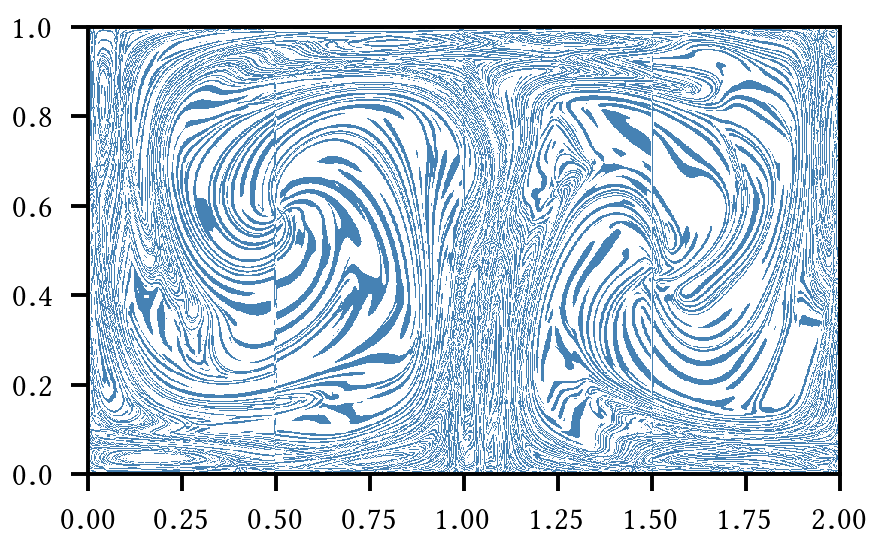
\includegraphics{figures/domain_figures/rkbs32_err_half_width.png}
        \caption[]{{\small Bogacki-Shampine 3(2)}}
        \label{fig:u0_dom_err_bs32}
    \end{subfigure}
    \begin{subfigure}[b]{0.475\textwidth}
        \centering
        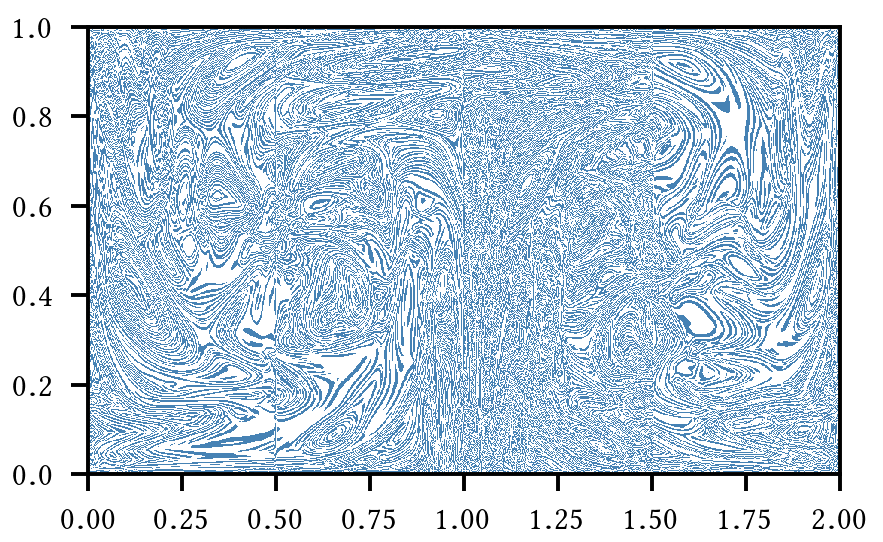
\includegraphics{figures/domain_figures/rkbs54_err_half_width.png}
        \caption[]{{\small Bogacki-Shampine 5(4)}}
        \label{fig:u0_dom_err_bs54}
    \end{subfigure}

    \begin{subfigure}[b]{0.475\textwidth}
        \centering
        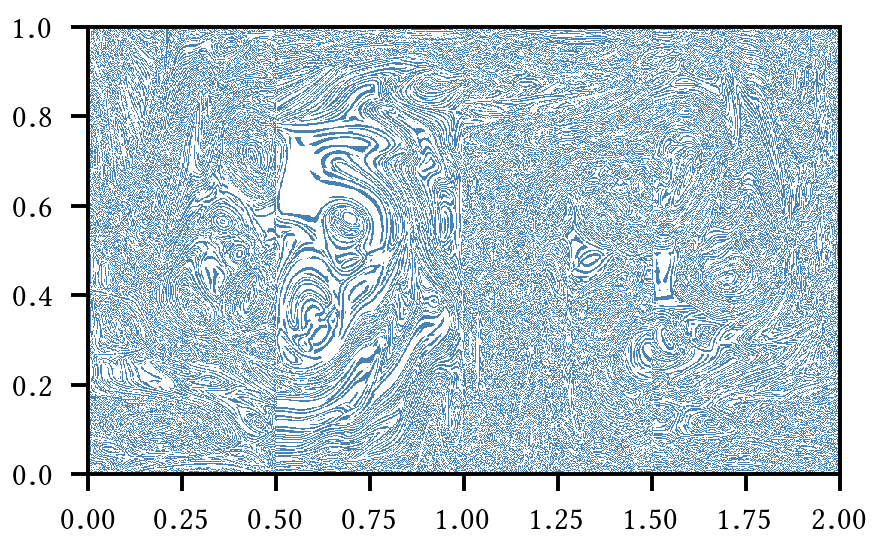
\includegraphics{figures/domain_figures/rkdp54_err_half_width.png}
        \caption[]{{\small Dormand-Prince 5(4)}}
        \label{fig:u0_dom_err_dp54}
    \end{subfigure}
    \begin{subfigure}[b]{0.475\textwidth}
        \centering
        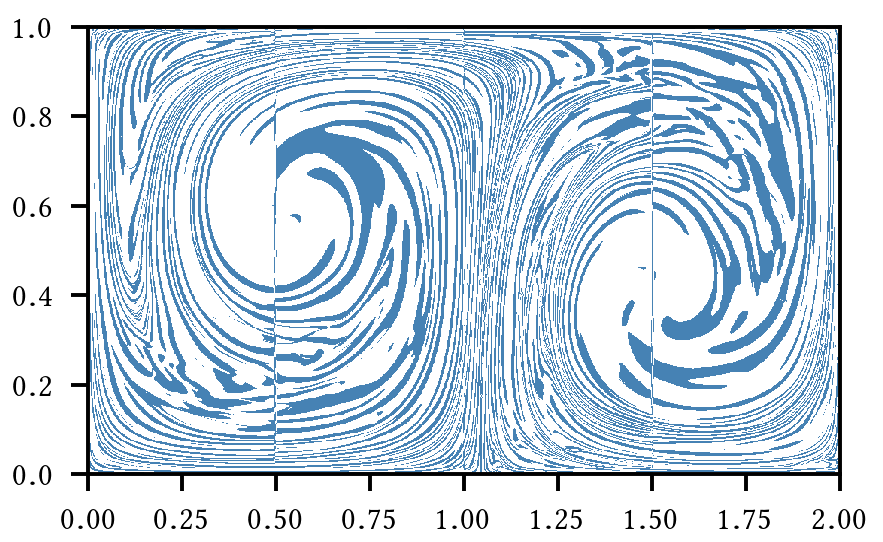
\includegraphics{figures/domain_figures/rkdp87_err_half_width.png}
        \caption[]{{\small Dormand-Prince 8(7)}}
        \label{fig:u0_dom_err_dp87}
    \end{subfigure}
    \caption[The $\mathcal{U}_{0}$ domains obtained with the adaptive stepsize
    integration schemes, with numerical tolerance level
    $\textnormal{tol}=10^{-1}$]{
        The $\mathcal{U}_{0}$ domains obtained with the adaptive stepsize
        integration schemes, with numerical tolerance level
        $\textnormal{tol}=10^{-1}$. Out of the four schemes considered, only the
    Dormand-Prince 8(7) method is remotely close to reproducing the
    reference domain, shown in~\ref{fig:u0_domain}. In any case, the
    differences are sufficiently large to alter the resulting strain
    system beyond recognition, rendering LCS comparisons with the reference
    impractical.}
    \label{fig:u0_dom_errs}
\end{figure}



\begin{table}[htpb]
    \centering
    \caption[Butcher tableau representation of the Bogacki-Shampine 3(2)
    embedded Runge-Kutta method]{Butcher tableau representation of the Bogacki-
    Shampine 3(2) embedded Runge-Kutta method. The $b$ coefficients correspond
to a \nth{3}-order accurate solution used to continue the integration. The
$\widehat{b}$ coefficients correspond to a \nth{2}-order accurate interpolant,
which can be used to estimate the error of the numerical approximation, and to
dynamically adjust the time step. The \emph{First Same As Last} property is
apparent from the fact that the $b$ coefficients correspond exactly to the
last row of coefficients in the Runge-Kutta matrix. For reference, see
\textcite{bogacki1989pair}.}
    \label{tab:butcherbs32}
    \renewcommand{\arraystretch}{2.5}
    \begin{tabular}{C|CCCC}
        \toprule
        0 & \\
        \dfrac{1}{2} & \dfrac{1}{2} \\
        \dfrac{3}{4} & 0 & \dfrac{3}{4} \\
        1 & \dfrac{2}{9} & \dfrac{1}{3} & \dfrac{4}{9} \\
        \hline
        & \dfrac{2}{9} & \dfrac{1}{3} & \dfrac{4}{9} \\
        \hline
        & \dfrac{7}{24} & \dfrac{1}{4} & \dfrac{1}{3} & \dfrac{1}{8} \\
        \bottomrule
    \end{tabular}
\end{table}

%\clearpage
\begin{table}[htpb]
\centering
    \caption[Butcher tableau representation of the Bogacki-Shampine 5(4)
    embedded Runge-Kutta method]{Butcher tableau representation of the Bogacki-
    Shampine 5(4) embedded Runge-Kutta method. The $b$ coefficients correspond
to a \nth{5} order accurate solution used to continue the integration. The
two rows of $\widehat{b}$ coefficients correspond to two independent \nth{4}
order accurate interpolants. They can be used to estimate the error of the
numerical approximation, and to dynamically adjust the time step. The fact that
two independent interpolants are included is a part of the reason for which
the method nearly behaves like a \nth{6} order method
\parencite[p.194 in the 2008 printing]{hairer1993solving}. The
\emph{First Same As Last} property is apparent from the fact that the $b$
coefficients correspond exactly to the last row of coefficients in the
Runge-Kutta matrix. For reference, see~\textcite{bogacki1996efficient}.}
    \label{tab:butcherbs54}
    \renewcommand{\arraystretch}{2.5}
    \begin{tabular}{C|CCCCCCCC}
        \toprule
        0 & \\
        \dfrac{1}{6} & \dfrac{1}{6} \\
        \dfrac{2}{9} & 0 & \dfrac{2}{27} & \dfrac{4}{27} \\
        \dfrac{3}{7} & \dfrac{183}{1372} & \dfrac{-162}{343} %
                     & \dfrac{1053}{1372} \\
        \dfrac{2}{3} & \dfrac{68}{297} & \dfrac{-4}{11} & \dfrac{42}{143} %
                     & \dfrac{1960}{3861} \\
        \dfrac{3}{4} & \dfrac{597}{22528} & \dfrac{81}{352} %
                     & \dfrac{63099}{585728} & \dfrac{58653}{366080} %
                     & \dfrac{4617}{20480} \\
        1 & \dfrac{174197}{959244} & \dfrac{-30942}{79937} %
          & \dfrac{8152137}{19744439} & \dfrac{666106}{1039181} %
          & \dfrac{-29421}{29068} & \dfrac{482048}{414219} \\
        1 & \dfrac{587}{8064} & 0 & \dfrac{4440339}{15491840} %
          & \dfrac{24353}{124800} & \dfrac{387}{44800} & \dfrac{2152}{5985} %
          & \dfrac{7267}{94080} \\
        \hline
          & \dfrac{587}{8064} & 0 & \dfrac{4440339}{15491840} %
          & \dfrac{24353}{124800} & \dfrac{387}{44800} & \dfrac{2152}{5985} %
          & \dfrac{7267}{94080} \\
        \hline
        & \dfrac{6059}{80640} & 0 & \dfrac{8559189}{30983680} %
        & \dfrac{26411}{124800} & \dfrac{-927}{89600} & \dfrac{443}{1197} %
                              & \dfrac{7267}{94080} \\
        & \dfrac{2479}{34992} & 0 & \dfrac{123}{416} & \dfrac{612941}{3411720} %
        & \dfrac{43}{1440} & \dfrac{2272}{6561} & \dfrac{79937}{1113912} %
        & \dfrac{3293}{556956} \\
        \bottomrule
    \end{tabular}
\end{table}

\begin{figure}[htpb]
    \centering
    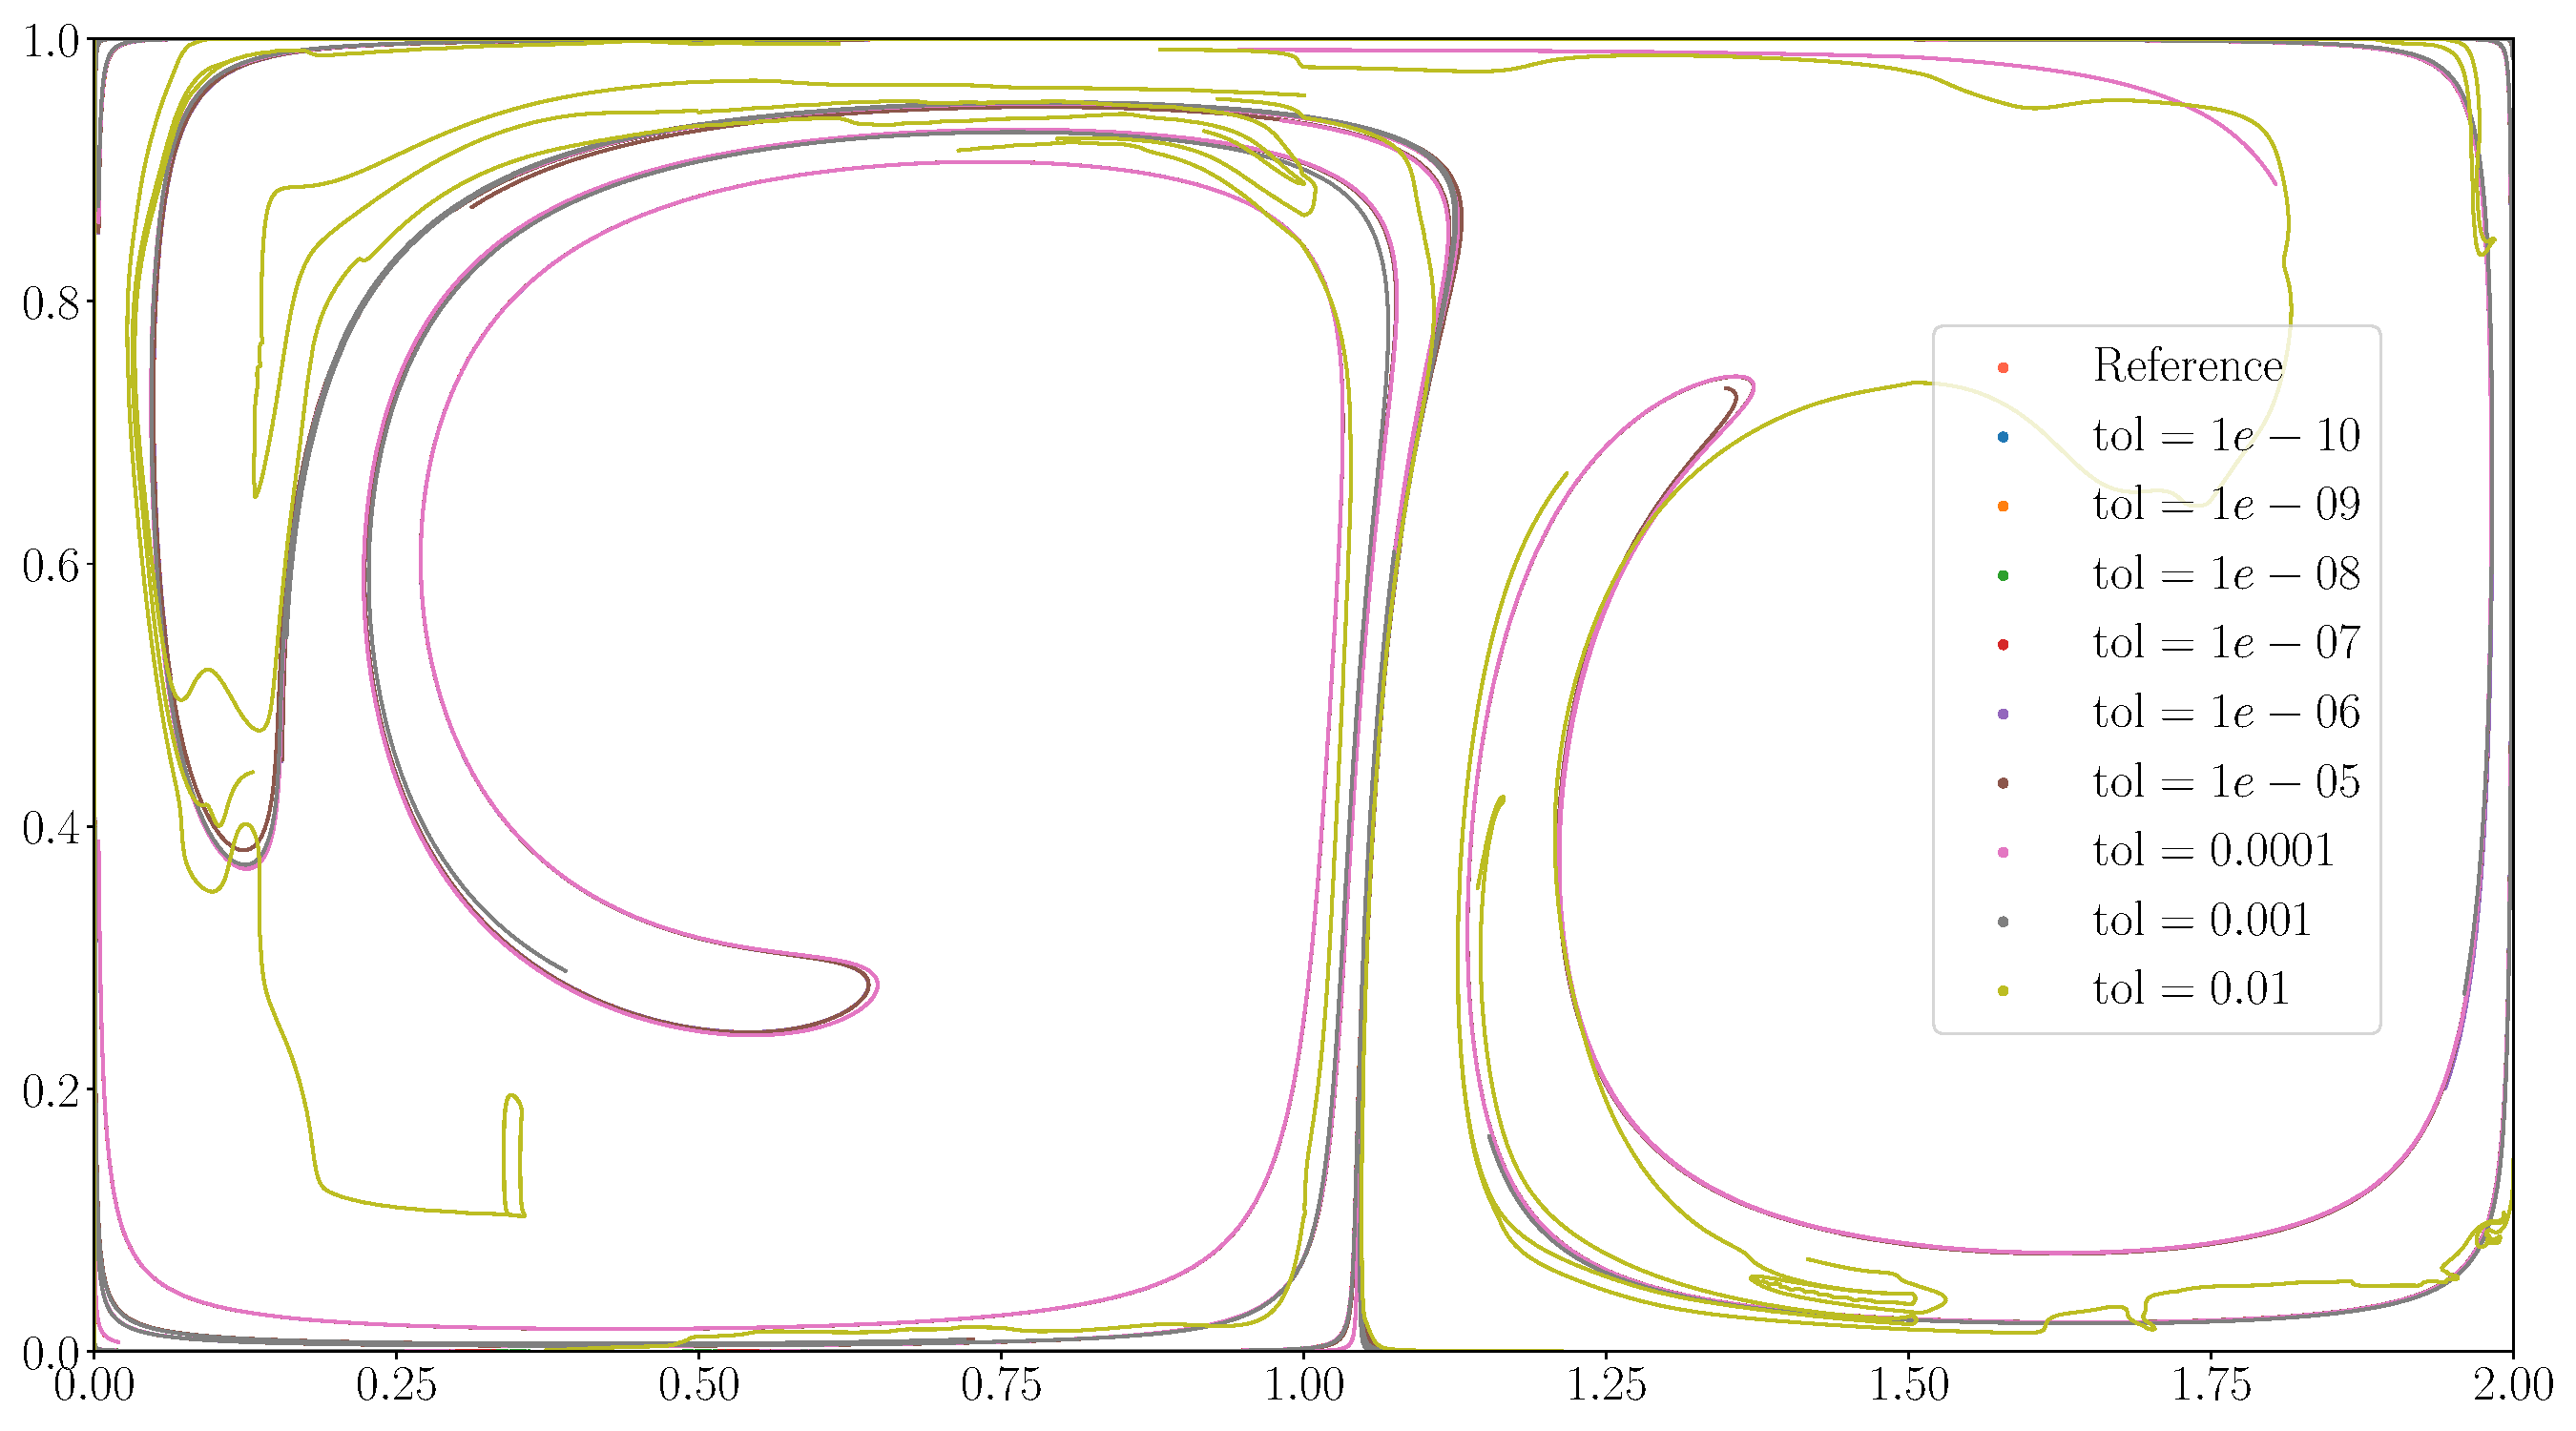
\includegraphics[width=0.9\linewidth]{figures/lcs_figures/rkdp54.pdf}
    \caption[LCS curves found by means of the Dormand-Prince 5(4) integration
    scheme]{
        LCS curves found by means of the Dormand-Prince 5(4) integration
        scheme. The reference LCS, as shown by itself in figure
        \ref{fig:referencelcs}, is plotted on the bottom layer. Note that
        the LCS for the lowest tolerance level considered, that is,
        $\textnormal{tol}=0.1$, is not included. This is because the
        corresponding $\mathcal{U}_{0}$ domain, shown in figure
        \ref{fig:u0_dp54}, and the reference $\mathcal{U}_{0}$, shown in figure
        \ref{fig:u0_domain} are dissimilar. Here, there are visible
        disparities for for all tolerance levels $\textnormal{tol}>10^{-6}$.}
    \label{fig:lcs_rkdp54}
\end{figure}


\begin{figure}[htpb]
    \centering
    \input{figures/lcs_figures/rkdp87.pgf}
    %\resizebox{0.9\linewidth}{!}{\input{figures/lcs_figures/rkdp87.pgf}}
    %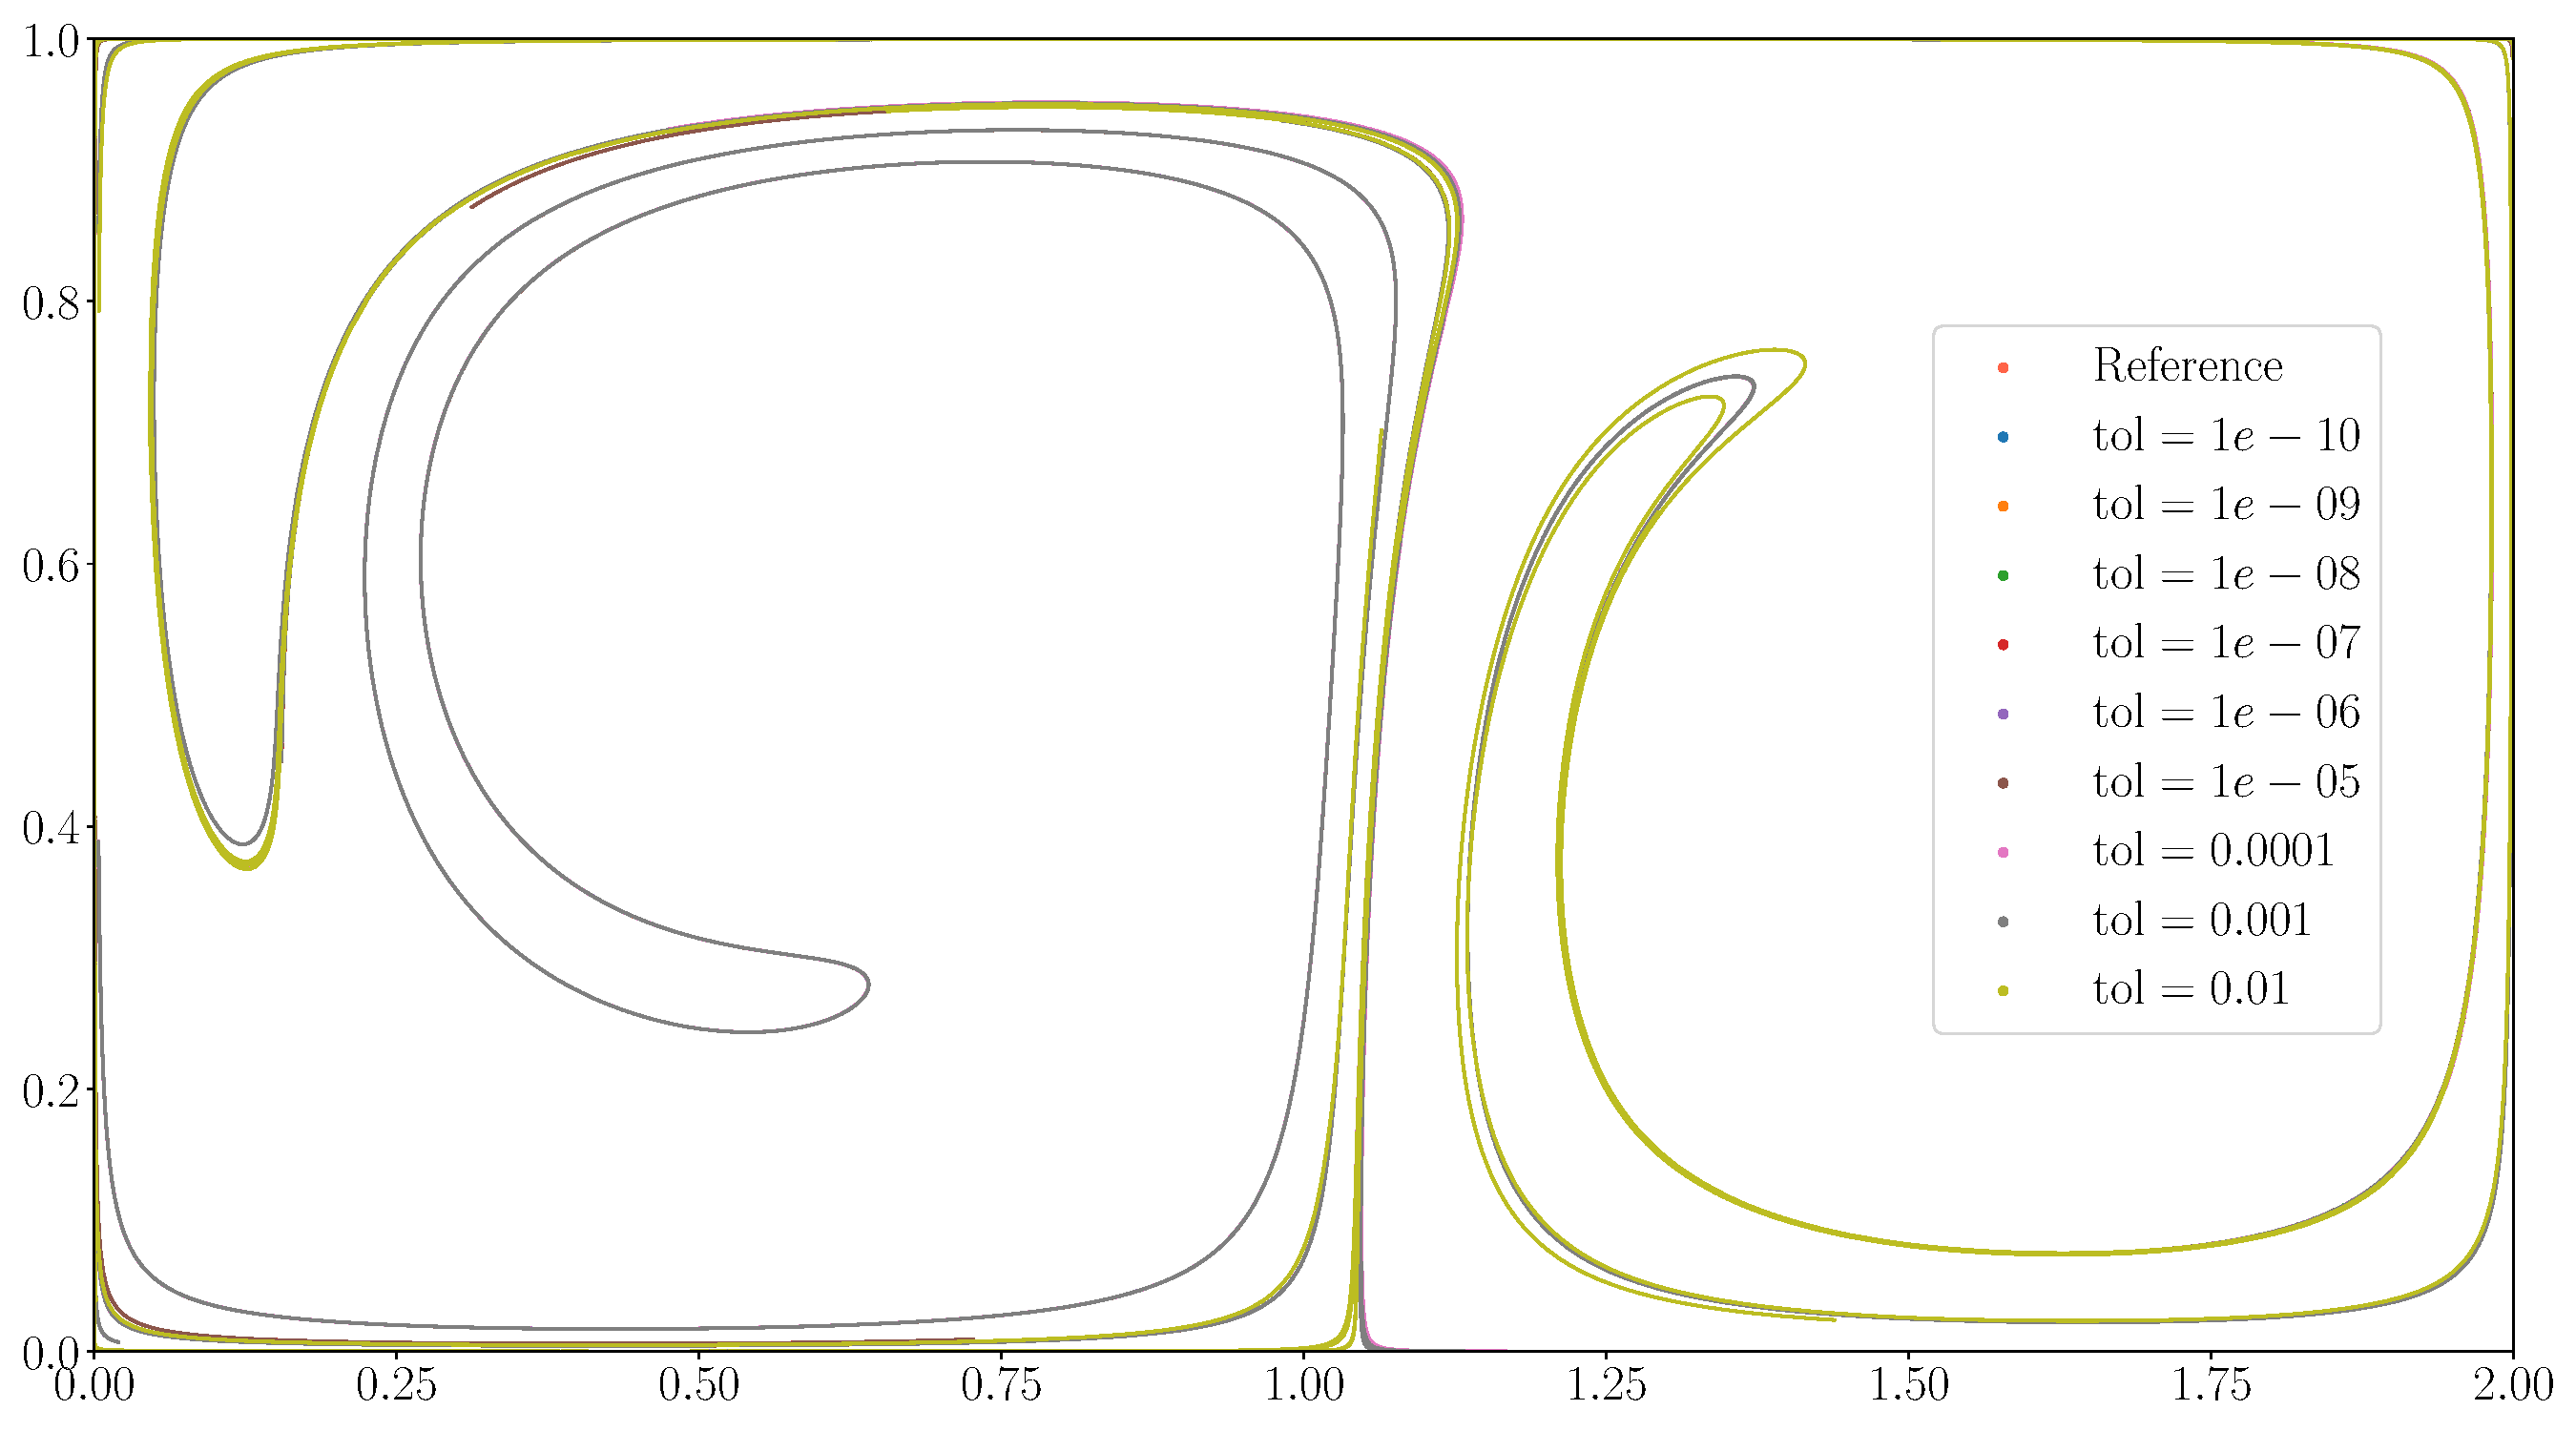
\includegraphics[width=0.9\linewidth]{figures/lcs_figures/rkdp87.pdf}
    \caption[LCS curves found by means of the Dormand-Prince 8(7) integration
    scheme]{
        LCS curves found by means of the Dormand-Prince 8(7) integration
        scheme. The reference LCS, as shown by itself in figure
        \ref{fig:referencelcs}, is dashed on the top layer. Note that
        the LCS for the lowest tolerance level considered, that is,
        $\textnormal{tol}=10^{-1}$, is not included. This is because the
        corresponding $\mathcal{U}_{0}$ domain, shown in figure
        \ref{fig:u0_dom_err_dp87}, and the reference $\mathcal{U}_{0}$, shown in figure
        \ref{fig:u0_domain} are quite unlike one another. Here, the most immediately
        discernible dissimilarities emanate from the tolerance level
    $\textnormal{tol}=10^{-2}$.}
    %Close inspection, however, reveals
    %    discrepancies for all tolerance levels $\textnormal{tol}>10^{-6}$,
    %    particularly by the `$\cap$' shape near $x=1.25$.}
    \label{fig:lcs_rkdp87}
\end{figure}





\section{Measures of error}
\label{sec:measures_of_error}

Here, the measures of error introduced in~\cref{sec:estimation_of_errors} for
the different numerical integration schemes considered, are presented. For
each different type of error, two figures are included. One in which the error
of the singlestep methods is shown as a function of the integration step length,
and one in which the error of \emph{all} the integration methods is shown
as a function of the number of times right hand side of the ordinary
differential equation system, that is, the velocity field given by
\cref{eq:doublegyre}, was evaluated for each step length or tolerance level.
The reason for which only the singlestep errors are included in the first set of
figures, is that they are the only methods where the error is expected to scale
as a power law in $h$, per \cref{def:rungekuttaorder}. This is naturally not the
case for the adaptive stepsize methods, where the step length varies.

More pertinent information can be found in the second set of figures, where
a well-suited integration method is characterized by generating small
errors at a small cost in terms of the required number of function calls,
in this case, the number of times the velocity field had to be evaluated.
Unlike the singlestep integrators, the advection of each tracer by means
of an adaptive stepsize method in principle requires a different number of
integration steps, and thus function evaluations. Thus, the presented number of
function evaluations is the \emph{average} across all of the advected tracers,
including the number of evaluations associated with rejected trial integration
steps. The number of function evaluations for each step of the considered
Runge-Kutta methods can be found as the number of rows in the Runge-Kutta
matrices of
\cref{tab:butchereuler,tab:butcherrk2,tab:butcherrk3,tab:butcherrk4,%
tab:butcherbs32,tab:butcherbs54,tab:butcherdopri54,tab:butcherdopri87}.
\subsection{Computed deviations in the flow maps}
\label{sub:computed_deviations_in_the_flow_maps}


Figure~\ref{fig:flowmap_err_fixed} indicates that the $\rmsd$ of the flow maps,
as defined in equation~\eqref{eq:rmsdflowmap} follow the expected power laws
of the numerical errors for the various singlestep integrators. This is
as expected, because the flow maps are found by direct application of the
numerical integrators. Furthermore, the flow map $\rmsd$ seem to exhibit
boundedness from below by the counteracting accumulated floating-point
arithmetic error, as hypothesized in
\cref{sub:on_the_choice_of_numerical_step_lengths_and_tolerance_levels}.
This effect is most prominent in the error curves of the Kutta and
classical Runge-Kutta schemes, which inflect upwards for sufficiently small
step lengths. Figure~\ref{fig:flowmap_err_both} indicates that this effect
did not materialize for the adaptive stepsize methods, for the considered
numerical tolerance levels.

Figure~\ref{fig:flowmap_err_both} reveals that the Bogacki-Shampine 3(2) scheme
is the `cheapest' in terms of the required number of function evaluations when
only a very crude approximation is needed, that is, using a very high
numerical tolerance level. Furthermore, the its higher order sibling is able
to keep up with the Dormand-Prince 8(7) method regarding efficiency, until
a mean of approximately $600$ function evaluations. This complies with the
notion that the Bogacki-Shampine 5(4) method is highly optimized and practically
behaves as an even higher order order method, as mentioned in
\cref{sub:the_runge_kutta_methods_under_consideration}.
Interestingly, there does not seem to be a direct correspondence between the
$\rmsd$ of the flow maps, and that of the computed LCS curves, presented in
\cref{sub:computed_deviations_in_the_lcs_curves}.

\input{mainmatter/results/figures/error_figures/flowmap_error_fixed_steplength.tex}

\input{mainmatter/results/figures/error_figures/flowmap_error_both.tex}

\subsection{Computed deviations in the strain eigenvalues and -vectors}
\label{sub:computed_deviations_in_the_strain_eigenvalues_and_vectors}

For brevity, only the $\rmsd$ of $\lambda_{2}$ and the direction of
$\vct{\xi}_{2}$, are included here. The latter is justified because of
the orthogonality of the eigenvectors of the Cauchy-Green strain tensor, which
means that the $\rmsd$ of the directions of both eigenvectors \emph{must} be
identical. Furthermore, the $\rmsd$ of $\lambda_{1}$ scales similarly to
that of $\lambda_{2}$, both as a function of numerical step length (for the
singlestep methods) and the number of function evaluations. Additionally, the
numerical reformulation of the existence theorem for hyperbolic LCSs, given in
\cref{eq:numericalexistence}, exhibits a more sensitive dependence to
$\lambda_{2}$ than $\lambda_{1}$. This is explicitly observable from
conditions~\eqref{eq:numericalexistence2} and~\eqref{eq:numericalexistence4},
and favors $\lambda_{2}$ as the most crucial eigenvalue.

Figure~\ref{fig:lmbd2_err_fixed} indicates that the $\rmsd$ of $\lambda_{2}$,
as defined in~\cref{eq:rmsdlmbd}, follows the anticipated scalings with the
step lengths for the various singlestep integrators. Interestingly, the $\rmsd$
dependence on the numerical step length is completely analogous to that of the
$\rmsd$ of the flow maps, as presented in
\cref{sub:computed_deviations_in_the_flow_maps}. Furthermore, inspection of
figure~\ref{fig:lmbd2_err_both} reveals that the $\rmsd$ of the $\lambda_{2}$
scales similarly to the $\rmsd$ of the flow maps for all of the integration
schemes, differing only by a numerical prefactor. This makes sense, seeing as
the calculation of the Cauchy-Green strain tensor field is based upon
finite differencing applied to the flow map, as described in
\cref{sec:calculating_the_cauchy_green_strain_tensor}.

\input{mainmatter/results/figures/error_figures/lmbd2_error_fixed_steplength.tex}

\input{mainmatter/results/figures/error_figures/lmbd2_error_both.tex}

\vspace{\fill}
\newpage

\Cref{fig:xi2_err_fixed} reveals that the $\rmsd$ of the eigenvector direction,
as defined in~\cref{eq:rmsddirection}, follows the anticipated scalings with
the step lengths for the various singlestep integrators to some degree. The
$\rmsd$ dependence on the numerical step length is not entirely analogous to
that of the $\rmsd$ of $\lambda_{2}$. Notably, the error in the eigenvector
directions is two to three orders of magnitude smaller than the error
in $\lambda_{2}$, for any given step size. This can be understood as a
consequence of using the auxiliary tracers in order to compute the strain
eigenvectors, as described in
\cref{sec:calculating_the_cauchy_green_strain_tensor}, which, by construction,
is more accurate than using the main tracers (which are used to
compute the strain eigenvalues). \Cref{fig:xi2_err_both} shows that the $\rmsd$ of
the eigenvector direction behaves qualitatively like that of the
$\rmsd$ of $\lambda_{2}$ (see~\cref{fig:lmbd2_err_both}) as a function
of the required number of function evaluations for each integration scheme.
Like for the singlestep methods, the $\rmsd$ of the eigenvector direction for
the embedded methods is generally between two and three orders of magnitude
smaller than the $\rmsd$ of $\lambda_{2}$ for any given number of function
evaluations.

%Figure~\ref{fig:xi2_err_fixed} reveals that the $\rmsd$ of the eigenvector
%direction, as defined in~\cref{eq:rmsddirection}, is negligible for
%all numerical step lengths. In fact, the numerical errors are comparable
%to, or even smaller than, the machine epsilon of double-precision floating-point
%numbers, which, as mentioned in
%\cref{sub:generating_a_set_of_initial_conditions}, is of order $10^{-16}$
%\parencite{ieee2008standard}. Because these errors are so small, the agreement
%with the anticipated scalings with the stepsize should not necessarily be taken
%as conclusive evidence of general behaviour. Figure~\ref{fig:xi2_err_both},
%shows that this is in fact the case for the adaptive stepsize methods too,
%aside from the tolerance level $\textnormal{tol}=10^{-1}$, which corresponds to
%the fewest function evaluations for each scheme. As has already been
%established in figure \ref{fig:u0_dom_errs}, for that tolerance level, none of
%the integrators yield $\mathcal{U}_{0}$ domains with reasonable degrees of
%resemblance to the reference, which is shown in figure~\ref{fig:u0_domain}.
%
From \cref{fig:lmbd2_err_both,fig:xi2_err_both}, it is clear that the
$\rmsd$s of $\lambda_{2}$ and the eigenvector direction are both quite large
for the tolerance level $\textnormal{tol}=10^{-1}$ (corresponding to the
smallest number of function evaluations) for all of the embedded methods.
This seems reasonable, given the erroneous $\mathcal{U}_{0}$ domains
obtained for that tolerance level, shown in~\cref{fig:u0_dom_errs} (compare
to~\cref{fig:u0_domain}). Moreover, the sharp turns which are present in
some of the computed LCS curves, perhaps most prominently in
\cref{fig:lcs_rkbs54,fig:lcs_rkdp54} for the tolerance level
$\textnormal{tol}=10^{-2}$, are likely a consequence of the error in the
eigenvalues and -vectors being sufficient for the corresponding
$\mathcal{U}_{0}$ domains to extend to regions in which there are very
strong local orientational discontinuities in the $\vct{\xi}_{1}$-field.
There, the special-purpose linear interpolation introduced in
\cref{sub:a_framework_for_computing_smooth_strainlines} is evidently
insufficient for computing smooth strainlines.

%Aside from the least accurate tolerance level for the embedded integrators,
%though, the error in eigenvector direction is comparable to, or smaller than,
%double-precision machine epsilon. Thus, we may conclude that the eigenvector
%directions are computed correctly for just about any tolerance level and
%numerical time step length. This can be understood as a consequence of the use
%of the auxiliary tracers in order to compute the strain eigenvectors, as
%described in~\cref{sec:calculating_the_cauchy_green_strain_tensor}, which, by
%construction, is more accurate than using the main tracers. Moreover, these
%results imply that the error in the resulting LCS curves are strongly driven by
%the error in the computed eigenvalues. The sharp turns in the computed LCS
%curves for the tolerance level $10^{-2}$, which are particularly visible
%in~\cref{fig:lcs_rkbs54,fig:lcs_rkdp54}, are likely a consequence of the
%corresponding $\mathcal{U}_{0}$ domains extending to regions in which
%there are very strong local orientational discontinuities in the
%$\vct{\xi}_{1}$-field, for which the special-purpose linear interpolation
%introduced in~\cref{sub:a_framework_for_computing_smooth_strainlines} is
%evidently insufficient.
%
\input{mainmatter/results/figures/error_figures/xi2_error_fixed_steplength.tex}


\input{mainmatter/results/figures/error_figures/xi2_error_both.tex}

%\clearpage

\subsection{Computed deviations in the LCS curves}
\label{sub:computed_deviations_in_the_lcs_curves}

Figures~\ref{fig:lcs_err_fp_fp} and~\ref{fig:lcs_err_fn_fn} indicate that
the integrated offset of false positives and negatives, as defined in
\cref{eq:midpointfalselcs}, is a decreasing function of the number of
function evaluations for all integration schemes. Moreover, the issue of false
positives and negatives vanishes entirely for sufficiently many function
evaluations, that is, sufficiently small numerical step lengths or tolerance
levels. This conforms well with the visual representations of the various
approximations of the LCS curve, as shown in
\cref{sec:the_lcs_curves_obtained_using_the_different_schemes}.
%, in addition
%to providing an indication that the LCS present in the double gyre system is
%robust, as long as all integration steps are sufficiently small in order to
%resolve the micro-scale behaviour .

Note that the offset of false positives and negatives has not been plotted as a
function of numerical time step for the singlestep methods. As can be seen from
\cref{fig:lcs_err_fp_fp,fig:lcs_err_fn_fn}, only the Euler method results in
false positives or negatives for more than one of the considered integration
step lengths, meaning that there are simply too few data points to identify
correlations between these numerical errors and the time step, cf.\
\cref{def:rungekuttaorder}. Moreover, there is no clear reason why these offsets
should scale similarly as, for instance, the errors in the computed flow maps
(see~\cref{sub:computed_deviations_in_the_flow_maps}).
Furthermore, offsets for the adaptive stepsize methods are not included for the
tolerance levels $10^{-1}$, because the LCS identification proved to be
exceedingly demanding in terms of computations for those cases, as described in
\cref{sub:lcs_curves_stemming_from_adaptive_stepsize_methods}. However,
based on the associated $\mathcal{U}_{0}$ domains, shown in figure
\ref{fig:u0_dom_errs}, one may infer an overwhelming probability of a large
number of false positives and negatives to be present, seeing as the underlying
strain systems are quite clearly different to the reference, shown in
figure~\ref{fig:u0_domain}.


\input{mainmatter/results/figures/error_figures/lcs_false_positives.tex}
\input{mainmatter/results/figures/error_figures/lcs_false_negatives.tex}
\clearpage


Figures~\ref{fig:lcs_rmsd_fp_nn_fixed} and~\ref{fig:lcs_rmsd_fn_nn_fixed} indicate
that the $\rmsd$ of the LCS curves, as defined in~\cref{eq:rmsdlcs},
does not follow the expected scalings of the numerical errors with the
stepsize for the various singlestep integrators. Moreover, the two measures of
the $\rmsd$ show the same quantitative behaviour, which is to be expected. The
error quickly flattens for all integrators except the Euler scheme, which agrees
well with the LCS curves presented in
\cref{fig:lcs_rk2,fig:lcs_rk3,fig:lcs_rk4}, where there are no visible
discrepancies with regards to the reference LCS curve for step lengths smaller
than $10^{-2}$. The fact that the $\rmsd$ of the curves obtained
by means of the Euler method appears to have flattened at a higher level than
the rest of the integrators implies that the Euler method will never result in
LCS curves with similar degrees of accuracy as for the other schemes. Lastly,
the sudden drop in $\rmsd$ for the other methods for the transition
$h=10^{-4}\rightarrow{h=10^{-5}}$ is unexpected. There is no clear reason for
why it occurs. A similar effect is not present in the $\rmsd$s of the
flow map, eigenvalues nor eigenvectors, shown in
\cref{fig:flowmap_err_fixed,fig:lmbd2_err_fixed,fig:xi2_err_fixed}.

\input{mainmatter/results/figures/error_figures/lcs_fp_nn_error_fixed_steplength.tex}

Figures~\ref{fig:lcs_rmsd_fp_nn_both} and~\ref{fig:lcs_rmsd_fn_nn_both}
show the $\rmsd$ of the LCS curves for all numerical integration methods as a
function of the required number of function evaluations per advected tracer.
For the adaptive stepsize methods, the error decreases steadily
with the number of function evaluations until a certain point, after which
the error suddenly jumps to the same steady level as the (high order)
singlestep methods. Like the sudden drop in the error for the singlestep
methods with a large number of function evaluations (i.e., for very
small time steps), there is no obvious reason why this jump occurs. Neither
does a similar trend manifest itself in the $\rmsd$s of the flow map,
eigenvalues or -vectors, as shown in
\cref{fig:flowmap_err_both,fig:lmbd2_err_both,fig:xi2_err_both}. Finally,
\cref{fig:lcs_rmsd_fp_nn_both,fig:lcs_rmsd_fn_nn_both} suggest that the
Bogacki-Shampine 5(4) and Dormand-Prince 8(7) schemes provide the overall most
efficient means of obtaining accurate LCS curves for the considered double gyre
system, in terms of the number of function evaluations needed to reach a given
level of precision.

\input{mainmatter/results/figures/error_figures/lcs_fn_nn_error_fixed_steplength.tex}

%\clearpage

\input{mainmatter/results/figures/error_figures/lcs_fp_nn_error_both.tex}

\input{mainmatter/results/figures/error_figures/lcs_fn_nn_error_both.tex}
\clearpage
%Figures~\ref{fig:lcs_rmsd_fp_nn_both} and~\ref{fig:lcs_rmsd_fn_nn_both}
%show the $\rmsd$ of the LCS curves for all numerical integration methods as a
%function of the required number of function evaluations per advected tracer.
%Interestingly, for the adaptive stepsize methods, the error decreases steadily
%with the number of function evaluations until a certain point, after which
%the error suddently jumps to the same steady level as the (high order)
%singlestep methods. As for the sudden drop in the error for the high order
%singlestep methods for sufficiently many function evaluations (i.e., for
%sufficiently small timesteps), there is no obvious reason why this occurs,
%seeing as a similar trend is not found in the $\rmsd$s of the flow map,
%eigenvalues and eigenvectors, as shown in figures
%\cref{fig:flowmap_err_both,fig:lmbd2_err_both,fig:xi2_err_both}.
%
%Finally, \cref{fig:lcs_rmsd_fp_nn_both,fig:lcs_rmsd_fn_nn_both} suggest that the high
%order adaptive stepsize methods, in particular the Bogacki-Shampine 5(4) and
%Dormand-Prince 8(7) schemes, provide the overall most efficient means of
%obtaining accurate LCS curves for the considered double gyre system, in terms
%of the required number of function evalations in order to obtain a given
%level of numerical error.
%
%
%\ref{fig:lcs_rmsd_fp_nn_both} and~\ref{fig:lcs_rmsd_fn_nn_both}, in that, the
%$\rmsd$ of the higher-order methods decreases steadily, until a certain point
%where it suddenly jumps to the same steady level as the (high order) singlestep
%methods. The most reasonable explanation is that when the number of function
%evaluations reaches some threshold, the accumulated floating-point arithmetic
%errors gain a larger influence than the inherent precision of the integrators.
%By similar logic, the sudden drop in $\rmsd$ for the high order singlestep
%methods with numerical step length $h=10^{-5}$, as can be seen in
%\cref{fig:lcs_rmsd_fp_nn_fixed,fig:lcs_rmsd_fn_nn_fixed}, is most likely an
%artifact of the random nature of the accumulated floating-point errors,
%moreso than a sudden `re-manifestation' of the inherent integrator accuracy.
%Finally, \cref{fig:lcs_rmsd_fp_nn_both,fig:lcs_rmsd_fn_nn_both} suggests that
%the high order adaptive stepsize methods, namely the Bogacki-Shampine 5(4) and
%Dormand-Prince 8(7) schemes, provide the most efficient means of obtaining
%accurate LCS curves for the considered double gyre system.
%\clearpage




%\vspace{\fill}

%\newpage
\addtocontents{toc}{\vspace{\fill}\protect\pagebreak}
\chapter{Discussion}
\label{cha:discussion}
\section{Remarks on the computed LCSs}
\label{sec:general_remarks}

Overall, the use of a variational framework for computing LCSs appears to
produce robust and consistent LCS curves for all of the numerical integration
schemes considered here, subject to usage of a sufficiently small numerical
step length or tolerance level. This is apparent from the LCS curves shown
in~\cref{fig:lcs_euler,fig:lcs_rk2,fig:lcs_rk3,fig:lcs_rk4,fig:lcs_rkbs32,%
fig:lcs_rkbs54,fig:lcs_rkdp54,fig:lcs_rkdp87} conforming visually with the
reference LCS, and the computed errors in the various LCS curves --- shown
in~\cref{fig:lcs_rmsd_fp_nn_both,fig:lcs_rmsd_fn_nn_both} --- being small.
Furthermore, this indicates that calculations of this kind
are not particularly sensitive to integration method. Note that the
$\mathcal{U}_{0}$ domains obtained by means of the adaptive stepsize methods
for $\textnormal{tol}=10^{-1}$, shown in figure~\ref{fig:u0_dom_errs}, differ
greatly from the reference domain (see~\cref{fig:u0_domain}), which correlates
well with the computed $\rmsd$ of the flow maps, shown in
figure~\ref{fig:flowmap_err_both}. In particular, the error in the flow map for
the aforementioned tolerance level is of order $1$ for all of the embedded
methods. This error is comparable to the extent of the numerical domain, that
is, $[0,\hspace{0.5ex}2]\times[0,\hspace{0.5ex}1]$. Naturally, this leads to a
drastically different system.

The above observation implies that the most crucial part of the computation is
advecting the tracers accurately. As mentioned in
\cref{sub:computed_deviations_in_the_strain_eigenvalues_and_vectors}, the errors
in the computed strain eigenvalues and -vectors scale like the error in the
computed flow map. This is to be expected, as the eigenvalues and -vectors are
essentially found by applying finite differences to the flow map. The
eigenvalues are crucial in terms of identifying LCSs, as can be seen in the
numerical reformulation of the LCS existence theorem, which is given in
\cref{eq:numericalexistence}. The error in the computed strain eigenvectors, is
consistently two to three orders of magnitude smaller than the error in the
eigenvalues. This is most likely due to them being computed based on the %denser
\emph{auxiliary} set of tracers, which per construction results in more accurate
finite differences.

From inspection of~\cref{fig:lcs_rmsd_fp_nn_fixed,fig:lcs_rmsd_fn_nn_fixed,%
fig:lcs_rmsd_fp_nn_both,fig:lcs_rmsd_fn_nn_both}, it becomes clear that the
error of the strainline components identified as LCS constituents, for some
configurations with small step lengths or tolerance levels, is dominated by
a seemingly constant contribution of the order $10^{-4}$. For instance,
for the Dormand-Prince 8(7) method,
\cref{fig:lcs_rmsd_fp_nn_both,fig:lcs_rmsd_fn_nn_both} show that for the three
lowest tolerance levels $\textnormal{tol}=10^{-8}$, $10^{-9}$ and
$10^{-10}$, respectively, the $\rmsd$ is of order $10^{-4}$, whereas it is
considerably smaller --- of order $10^{-7}$ --- for $\textnormal{tol}=10^{-7}$.
This is unexpected, as we expect the error to decrease when the tolerance level
is lowered.  Notably, this occurs for larger step lengths or tolerance levels,
respectively, than the corresponding turning points for the error in the flow
maps (i.e., the points at which the error in the flow maps increases with
decreasing step length or tolerance level). However, close inspection of
\cref{fig:lcs_rk2,fig:lcs_rk3,fig:lcs_rk4,fig:lcs_rkbs32,fig:lcs_rkbs54,%
fig:lcs_rkdp54,fig:lcs_rkdp87} reveals that, for the numerical step lengths
and tolerance levels which correspond to the same level of error in the LCS
curves (see~\cref{fig:lcs_rmsd_fp_nn_fixed,fig:lcs_rmsd_fn_nn_fixed,%
fig:lcs_rmsd_fp_nn_both,fig:lcs_rmsd_fn_nn_both}), the computed LCS
approximations are made up of seven different strainline segments each. This
is unlike the reference LCS, which, as previously mentioned, consists
of \emph{eight} strainline segments.
\clearpage
\Cref{fig:lcserroroscillations} shows the computed LCS approximations together
with the reference LCS, for the Dormand-Prince 8(7) method with tolerance
levels $\textnormal{tol}=10^{-5}$ through to $\textnormal{tol}=10^{-8}$ ---
the tolerance levels for which oscillations are visible in the computed errors
of the LCS curves (see~\cref{fig:lcs_rmsd_fp_nn_both,fig:lcs_rmsd_fn_nn_both})
--- for a subset of the computational domain $\mathcal{U}$. Notice in
particular that the second reference LCS curve segment (counting from the top
and downwards) is present in the approximations for $\textnormal{tol}=10^{-5}$
and $10^{-7}$, but \emph{not} for $\textnormal{tol}=10^{-6}$ and $10^{-8}$.
However, the two topmost reference LCS curve segments shown in the figure
are sufficiently close for this error not to be identified as a false negative.
Thus, when computing the LCS $\rmsd$, the offset between the LCS curve segment
corresponding to the topmost one shown in the figure, and the second topmost
reference LCS curve likely dominates the other contributions. Furthermore, the
fact that this offset is nearly constant explains the apparently identical LCS
$\rmsd$ in the cases where the computed LCS approximation consists of seven
strainline segments (as shown in
\cref{fig:lcs_rmsd_fp_nn_fixed,fig:lcs_rmsd_fn_nn_fixed,%
fig:lcs_rmsd_fp_nn_both,fig:lcs_rmsd_fn_nn_both}). For all of the numerical step
lengths and tolerance levels which result in the same level of LCS $\rmsd$, the
situation is the same as for the  tolerance levels $\textnormal{tol}=10^{-6}$
and $\textnormal{tol}=10^{-8}$, shown in~\cref{fig:lcserroroscillations}. Figures
showing the same level of  detail for the remaining integration methods have
thus been omitted for brevity. Note that the two reference LCS curve
segments in question nearly overlap, and their $\overline{\lambda}_{2}$ differ
by less than 5\%; thus, the absence of the second topmost reference LCS curve
segment would likely not have severe consequences for predictions regarding
the overall flow in the system.

\begin{figure}[htpb]
    \centering
    \input{figures/error_figures/lcs_error_oscillations.pgf}
    \caption[A possible explanation for the behaviour of the $\rmsd$ of the
    computed LCS curves]
    {A possible explanation for the behaviour of the
        $\rmsd$ of the computed LCS curves. The computed LCS curves obtained by
        means of the Dormand-Prince 8(7) method, for tolerance levels
        $\textnormal{tol}=10^{-5}$ through to $\textnormal{tol}=10^{-8}$, are shown
        (solid) together with the reference LCS (dashed) for a subset of the
        computational domain $\mathcal{U}$. Notice how the second reference LCS
        curve segment (counting from the top and downwards) is present in the LCS
        approximations obtained for $\textnormal{tol}=10^{-5}$ and
        $\textnormal{tol}=10^{-7}$, but \emph{not} for $\textnormal{tol}=10^{-6}$
    and $\textnormal{tol}=10^{-8}$. The offset between the between the two
topmost reference LCS curve segments shown in the figure is too small for the
absence of the second topmost reference LCS curve segment to be flagged as a
false negative. For all numerical step lengths and tolerance levels which
correspond to the same level of $\rmsd$ in the computed LCS curves
(see~\cref{fig:lcs_rmsd_fp_nn_fixed,fig:lcs_rmsd_fp_nn_both,%
fig:lcs_rmsd_fn_nn_fixed,fig:lcs_rmsd_fn_nn_both}), the second topmost reference
LCS curve segment is not present in the LCS approximation. For those cases,
the offset between the analogue to the topmost one shown in this figure, and
the second topmost reference LCS curve segment is approximately constant, and
likely dominates any other errors --- which leads to the flattening of the
$\rmsd$, visible in~\cref{fig:lcs_rmsd_fp_nn_fixed,fig:lcs_rmsd_fp_nn_both,%
fig:lcs_rmsd_fn_nn_fixed,fig:lcs_rmsd_fn_nn_both}.}
    \label{fig:lcserroroscillations}
\end{figure}


Following the above discussion, the results obtained here do not indicate
the existence of a lower sufficiency threshold in terms of the required
advection accuracy, beneath which the computed LCS curves do not become more
precise. Any such threshold would, however, likely only be valid for the LCS
curves of this particular velocity field --- that is, the system given by
\cref{eq:doublegyre,eq:doublegyrefuns,eq:doublegyreparams} --- which
appear quite robust overall. Other, more volatile systems, would probably
require more accurate advection. However, investigating this further for a
wider range of systems could result in valuable insight. Should such an
advection threshold exist, and be linked to the scales of the given system,
it would naturally be of great significance when investigating generic transport
systems by means of a similar variational LCS approach. Admittedly, there is no
apparent reason why this should be the case.

%For the considered double gyre system, there appears to be a lower threshold
%in terms of the required advection accuracy, beneath which the computed LCS
%curves do not become more precise. This effect is apparent
%from inspection of
%\cref{fig:lcs_rmsd_fp_nn_fixed,fig:lcs_rmsd_fn_nn_fixed,%
%fig:lcs_rmsd_fp_nn_both,fig:lcs_rmsd_fn_nn_both}, where the error of strainline
%components identified as LCS constituents flattens abruptly. Notably, this
%occurs for larger numerical step lengths or tolerance levels, respectively,
%than the corresponding turning points for the error in the flow maps.
%For the double gyre system considered here, it appears that this advection
%accuracy threshold is of the order $10^{-6}$--$10^{-7}$, which follows from
%comparing~\cref{fig:lcs_rmsd_fp_nn_fixed,fig:lcs_rmsd_fn_nn_fixed,%
%fig:lcs_rmsd_fp_nn_both,fig:lcs_rmsd_fn_nn_both} to
%\cref{fig:flowmap_err_fixed,fig:flowmap_err_both}. In particular, for flow maps
%with $\rmsd$ of $10^{-7}$ or lower, the $\rmsd$ of the LCS curves appears to
%not decrease further as the flow map precision increases.
%
%However, because a similar flattening of the $\rmsd$ for the strain eigenvalues
%and eigenvectors is not apparent in
%\cref{fig:lmbd2_err_fixed,fig:lmbd2_err_both,fig:xi2_err_fixed,fig:xi2_err_both},
%one may infer that this threshold is likely only valid for the LCS curves
%of this particular velocity field --- that is, the system given by
%\cref{eq:doublegyre,eq:doublegyrefuns,eq:doublegyreparams} %
%%, for which LCSs are
%%found by means of the procedure described in
%%\cref{sec:advecting_a_set_of_initial_conditions,%
%%%    sec:calculating_the_cauchy_green_strain_tensor,%
%%%sec:identifying_lcs_candidates_numerically}
%--- which
%appear quite robust. The same flow map accuracy threshold probably does not
%suffice for other, more volatile flow systems. Investigating
%this further for a wider range of systems could result in valuable insight.
%Should such a threshold be valid in general, it would naturally be of great
%significance when investigating generic transport systems by means of a
%variational LCS approach. Admittedly, there is no apparent reason why
%this should be the case.
%
The double gyre model considered in this project is obviously not representative
of generic systems, in terms of the exact numerical step lengths or tolerance
levels necessary in order to obtain correct LCSs with a certain
degree of confidence. It does, however, indicate that these quantities should
be chosen based on the considered system. For a fixed stepsize integration
scheme, any single integration time step should not be so large that \emph{too}
much detail in the local and instantaneous velocity field is glossed over.
Similar logic applies when adaptive stepsize methods are used, although it
may be more difficult to enforce, depending on how the step length
update is implemented. One possibility in terms of choosing the time step, is to
find a characteristic velocity for the system, and choose the time step small
enough so that a tracer moving with the characteristic velocity never traverses
a distance greater than the grid spacing, when moving from one time level to
the next.
\clearpage
The computed reference LCS for the double gyre system considered here, shown in
\cref{fig:referencelcs}, is made up of \emph{eight} different strainline
segments. The LCS presented in the article by \textcite{farazmand2012computing}
is claimed to consist of a \emph{single} strainline segment. Comparing the two
curves visually, however, indicates that the resulting LCSs are similar.
Likewise, the domain $\mathcal{U}_{0}$, shown in figure~\ref{fig:u0_domain},
strongly resembles the one found by \citeauthor{farazmand2012computing}.
Nevertheless, the total number of points in the domain computed here is
approximately two percent larger than what \citeauthor{farazmand2012computing}
found. These discrepancies could originate from different conventions in terms
of generating the grid of tracers. Notably, \citeauthor{farazmand2012computing}
fail to provide a description of their approach.

When computing transport based on discrete data sets, such as snapshots of the
instantaneous velocity fields in oceanic currents, spatial and temporal
interpolation becomes necessary. Together with the inherent precision of the
model data, the choice of interpolation scheme(s) sets an upper bound
in terms of the accuracy with which tracers can be advected. For such cases,
the interaction between the integration and interpolation schemes could
be critical --- both in terms of computation time and memory requirements,
aside from the numerical precision. Independently of the scales at which
well-resolved LCS information is sought in this kind of system, the
aforementioned effects warrant further investigation.

%
\section{On the incompressibility of the velocity field}
\label{sec:on_the_incompressibility_of_the_velocity_field}

As explained in~\cref{sec:the_double_gyre_model}, the double gyre velocity field
is incompressible per construction. Thus, per equation
\eqref{eq:cauchygreenincomprlambda}, the product of the strain eigenvalues
should equal one. Regardless of the integration method used, however, this
property was lost after approximately five units of time. This is not
particularly surprising, because this property only really holds for
infinitesimal fluid elements. Seeing as there is no assurance that neighboring
tracers will remain nearby under the flow map, the finite difference
approximation to the local stretch and strain could practically be rendered
invalid. This issue is expected to be most prominent in regions of high local
repulsion, which are precisely where accuracy is most imperative.

Thus, one should not really expect this property to hold numerically, especially
for an indefinite time. However, sample tests indicate that the
incompressibility property was preserved for longer when using a denser
grid of tracers. In fact, the strain eigenvalue product was found to be unity
beyond 20 units of time, that is, the integration time used in this project,
for an initial grid spacing of $10^{-12}$. However, due to the inherent
inaccuracy of double-precision floating-point numbers, this would leave very
few significant digits with which one could perform finite differencing, as
mentioned in
\cref{sub:on_the_choice_of_numerical_step_lengths_and_tolerance_levels}.
In the end, the grid spacing $\Delta{x}\simeq\Delta{y}\simeq0.02$ was chosen,
because it was the resolution at which repelling LCS curves for the double
gyre system have previously been described in the literature, cf.
\textcite{farazmand2012computing}.

For further analysis, grid spacings of approximate order $10^{-7}$--$10^{-8}$
could be considered, when working with double-precision floating-point numbers.
This would probably result in the incompressibility property being preserved
for longer, while also leaving up to 7 or 8 significant digits for finite
differencing. An entirely different approach, as suggested by
\textcite{onu2015lcstool}, is to simply \emph{define} the smaller strain
eigenvalue as  the reciprocal of the larger one, that is,
$\lambda_{1}\equiv\lambda_{2}^{-1}$. This was not done here, because the
flow incompressibility has no obvious practical consequences for LCSs.
In addition, subject to the accuracy of the numerical integration scheme,
no tracer which starts out within the computational domain
$[0\hspace{1ex}2]\times[0\hspace{1ex}1]$ ever leave it, due to the normal
component of the velocity field being zero along the domain edges. This
follows from the definition of the associated velocity field, given in
equation~\eqref{eq:doublegyre}.

\vspace{\fill}


\section{Concerning the numerical representation of tracers}
\label{sec:concerning_the_numerical_representation_of_tracers}

One way of increasing the numerical accuracy in the flow map, would be
to use higher precision floating-point numbers to represent the tracer
coordinates. The main drawback of making such a change, is that this
neccessitates an increase in memory usage, which has the practical consequence
that less tracers can be advected at once. The immediately obvious workarounds
are to either use a high performance scientific computer, or to perform several
advections of smaller sets of tracers, calculating a piecewise representation
of the overall flow map. However, should this prove impossible, using higher
precision floating-point numbers leads to a more granular representation of the
flow map. Such an approach is perhaps most sensible for systems with velocity
fields that are well-behaved, or even largely spatially invariant. However,
in such cases, calculating LCSs have little practical relevance, seeing as
the overall behaviour of the flow system could be estimated purely by
advecting a smaller set of tracers, or even by simple inspection.

Rather than generating and advecting a fixed, large amount of tracer particles,
another possible approach would be to use a set of fewer `base' tracers, and
making use of an \emph{adaptive multigrid method}. A practical implementation
could involve the dynamic introduction of increasingly finer grids in regions
where the local velocities would have the largest Euclidean norm, for instance.
Such grids, however, would have to move \emph{with} the flow, as the
benefit over simply increasing the initial tracer density would diminish
otherwise. The main reason why this was not implemented for this project,
aside from it not being used in the literature, is that it in all likelyhood
leads to inconsistencies when applying finite differences. That is, unless some
sort of interpolation scheme was applied to the flow map. Seeing as this
project is centered around integration methods, this idea was scrapped.
Regardless, this technique seems promising --- at least on paper, which
warrants further investigation.


\section{Regarding the computation of strainlines}
\label{sec:regarding_the_computation_of_strainlines}
As outlined in~\cref{sub:a_framework_for_computing_smooth_strainlines}, a
special sort of rectifying linear interpolation routine was implemented in
order to eliminate local orientational discontinuities in the $\vct{\xi}_{1}$
strain eigenvector field. The logical next step would be to consider a larger
local subset of grid points, for instance, the $3\times3$ or $4\times4$ square
of the 9 or 16 nearest neighbors, respectively, systematically reorientating the
eigenvectors if necessary, and then using a higher order interpolation scheme
in order to approximate the local strain eigenvector. This sort of
generalization could make the strainline computation process more robust ---
although the linear approximation approach proved sufficient for the
velocity field considered here, that may not be the case for more complex or
volatile flow systems.

The classical Runge-Kutta method, with a numerical step length
$\Delta=10^{-3}$, was used for all computations of strainlines, regardless
of advection integration scheme. This was a conscious choice, based on the idea
of using the available information in the flow maps with the same degree of
precision for all integrator configurations. If, however, the entire process of
numerical integration, including both the advection of tracers and the
calculation of strainlines, were to be performed with the same integrator
configuration, comparisons between the resulting LCSs could have been
misleading. That in, the strain information present in the flow maps would
necessarily not have been utilized to the full extent, if the strainline
integration was performed by means of an imprecise integration scheme, i.e.,
for large time steps or tolerance levels. For instance, the LCSs curves obtained
by means of the Euler method, shown in figure~\ref{fig:lcs_euler}, could have
exhibited even more false positives and negatives if the same method was used
in order to obtain strainlines as well, due to it only being \nth{1}-order
accurate.

An alternative approach to the numerical integration of strainlines, would be
to make use of a high order adaptive step length method. This could, in
principle, reduce the required computational time, in addition to reducing
the impact of floating-point arithmetic error. However, in order to encapsulate
the local strain dynamics accurately, the embedded automatic step size control
should probably be more elaborate than the implementation outlined in
\cref{sub:on_the_implementation_of_embedded_runge_kutta_methods}. In particular,
it would be advisable to incorporate the local strainline curvature somehow,
in order to minimize deviations from the \emph{true} trajectories. Furthermore,
the use of a higher order strainline integration scheme might prove a fruitless
exercise, unless a higher order strain eigenvector interpolation routine, as
mentioned above, was implemented in tandem. This is because the effective
accuracy of the strainline integration method depends strongly on the
interpolation method, as evidenced by the reformulation of the basic
strainline ODE given in~\cref{eq:strainlinebasicode} to the ODE which
was used here, given in~\cref{eq:strainlineode}. As for the transport of tracers
based on discrete velocity data, mentioned in~\cref{sec:general_remarks}, the
interaction between strain eigenvector interpolation method, and strainline
integration method, seems like an interesting research topic for potential
future endeavors.

%
%\vspace{\fill}
%\clearpage


\section{The identification of strain maximizing strainlines}
\label{sec:the_identification_of_strain_maximizing_strainlines}

As mentioned in~\cref{sub:extracting_hyperbolic_lcss_from_strainlines},
the lines in the set $\mathcal{L}$, used in order to find strainline segments
satisfying the numerical LCS existence condition given in
\cref{eq:numericalexistence4} --- regarding the identification of strainlines
which serve as local maxima for $\overline{\lambda}_{2}$ --- had to be selected
with great care in order to accurately reproduce the LCS curve found in the
literature. Although the LCS identification with the particular set of
horizontal and vertical lines proved robust across all integration methods, the
fact that only certain sets $\mathcal{L}$ were found conducive to appropriate
strainline selection, is a damning indicament that the procedure as such is not
particularly robust. Although not investigated here, an alternative approach
could be to identify all strainlines which follow very similar trajectories,
either manually or by means of some numerical clustering algorithm, then
extracting the most strongly repellent strainline segments of each bunch as
LCSs for the system.

The strainline tail end cutting procedure which was employed, briefly brought
up in
\cref{sub:extracting_hyperbolic_lcss_from_strainlines} and illustrated in
\cref{fig:tailcutting}, is most certainly debatable. The reason it was
considered in the first place, is that the specific wording used by
\textcite{farazmand2012computing} on the subject of comparing strainlines is
somewhat ambiguous, in that they also describe that part of the process as
comparison of \emph{curve segments}. Moreover, they also state that a
\emph{part} of a strainline may qualify as an LCS. In addition, cutting the
tail ends of strainlines which are stopped due to continuous failures of one
or more of the LCS conditions given in
\cref{eq:numericalexistence} could also, quite logically, be extended so that
parts of the remaining strainline curve which, for example due to numerical
noise, do not satisfy all of the aforementioned conditions, are excluded from
the ensuing LCS identification. That is, those parts would not be considered
when computing the $\overline{\lambda}_{2}$, the averaged $\lambda_{2}$ of
the strainline segment, on the strainline as a whole, nor
the strainline length. Effectively, this could result in a strainline being
chopped into several shorter and disjointed segments, further resulting in
disjointed LCS curves. The aforementioned strainline tail end cutting proved
necessary in order to reproduce the LCS curve found by
\textcite{farazmand2012computing}, meaning that this concept can, and most
likely should, be investigated further.

Lastly, the rationale of filtering out LCS candidate curves which are shorter
than the preselected length $l_{\textnormal{f}}=1$, described in
\cref{sub:extracting_hyperbolic_lcss_from_strainlines} and inspired by
\textcite{farazmand2012computing}, was that excessively short LCSs are
expected to have a negligible impact on the overall flow in the system.
However, \citeauthor{farazmand2012computing} do not provide a justification
for why they chose that particular filtering length. Another way to perform this
sifting, would be to consider $\overline{\lambda}_{2}$ together with the length
of the strainline segment. This could be done in such a way that, when selecting
an LCS candidate from two strainlines, if one is somewhat longer but has a
slightly smaller $\overline{\lambda}_{2}$ (that is, is slightly less repelling
than, the other), then the longer strainline is selected. This sort of routine
should naturally be based upon sound mathematical logic. In short, there is a
lot of room for research in terms of how to enforce the LCS condition given
by~\cref{eq:numericalexistence4}. The conditions given by
\cref{eq:numericalexistence1,eq:numericalexistence2,eq:numericalexistence3}
are quite unambigious, in comparison.

%\vspace{\fill}
%\clearpage


\section{About the measures of error}
\label{sec:about_the_measures_of_error}

For all the measures of error introduced in~\cref{sec:estimation_of_errors},
except the one concerning false positives and negatives with regards to
LCS identification, a sort of averaging was utilized. Regarding the flow maps,
this choice was made based on the fact that it encapsulates the effect of
outliers, that is, any tracers for which the advection error becomes
relatively large. These are expected to have the most severe impact on the
ensuing LCS identification procedure. As shown in
\cref{fig:flowmap_err_fixed,fig:flowmap_err_both}, the errors of the Euler
method and all of the adaptive stepsize methods, for the largest numerical step
length and tolerance level, respectively, are of order 1, similar to the
dimensions of the computational domain, that is,
$[0\hspace{1ex}2]\times[0\hspace{1ex}1]$. However, because there is no general
a priori way of knowing the regions of the domain in which the flow maps will be
resolved the most poorly, the maximum error is not of particular interest
in this kind of analysis.

Because the normal component of the velocity field is zero at the domain
boundaries, one expects the flow map error to, in some sense, be limited from
above by the domain extent. Thus, one could argue that using the median error
as the measure in such cases would be more appropriate. This is clearly an
artifact of the particular velocity field, however. For a generic compressible
system, this need not be the case. For reasons of consistency, in addition to
the inclusion of the error of outliers, the $\rmsd$ was used as the measure of
error for all flow maps. Similar arguments apply for the other measures
of errors involving $\rmsd$. Moreover, each particular kind of error
is expected to follow some sort of statistical distribution. Although the
exact natures of the distribution have not been explored in detail in this
project, because the tracers are advected independently, each error in
the flow maps, for instance, can be considered as an independent
random variable. Because of the large numbers of individual data samples,
the $\rmsd$ can be considered a measure of the standard deviation of the
distribution of errors as a whole.

Regarding the estimation of the offset of falsely positively or negatively
identified LCS curves, there exists other measures of error.


%\begin{framed}
%    \begin{itemize}
%        \item \sout{Approach does produce a consistent LCS picture for all numerical integrators considered, provided sensible
%            integration steps or tolerance levels are chosen. This indicates that the calculation of this type
%        of transport barrier is not particularly sensitive to the integration method.}
%    \item \sout{Most crucial part: Compute advection correctly. The error of the computed strain eigenvalues scales
%                like the advection error, while the error in the strain eigendirections is negligible for all time
%                steps. The computed LCSs seem to exhibit sensitive dependence on the calculation of the eigenvalues,
%            which is not particularly surprising, considering the LCS conditions of eq. 3.13 }
%                \begin{itemize}
%                    \item \sout{The precision of the strain eigendirections is likely a direct consequence of the
%                        auxiliary tracers in their computation.}
%                \end{itemize}
%            \item \sout{The number of points in the $\mathcal{U}$ domain is different to the one obtained by
%                Haller et  al, by approximately $3\%$. This, however, is likely related to how the
%            grid of tracers was set up. In their paper, Farazmand and Haller do not provide details.}
%        \item \sout{Notably, the reference LCS as shown in figure (.) consists of seven different strainline
%                segments, unlike the structure found by Haller et al., which is claimed to be a single
%            coherent strainline.}
%
%        \item \sout{The time lenghts or tolerance levels should be chosen based on the system under consideration.
%            In particular, an individual time step should not be so large that too much detail in the local,
%        instantaneous velocity field is glossed over.}
%    \item \sout{Possible approach in order to refine the computations: Use fewer `base' tracers, and an \emph{adaptive multigrid method}. Main con: May lead to inconsistent centered differencing when approaching
%        the Jacobian etc. of the flow map}
%        \item \sout{Regarding the completely different domains obtained via the embedded methods for the highest tolerance level:
%            Check if this corresponds th the error in the flow map larger than some threshold. If (likely) so, this is
%        further evidence that one should exhert great effort in computing the flow map correctly.}
%    \item \sout{In terms of application to discrete velocity data sets, where both spatial and temporal interpolation
%                    may be necessary, the interaction between interpolation and integration scheme is likely to
%                    have a great overall impact. In particular, the underlying interpolation scheme sets a lower accuracy
%                    bound for the entire advection process, practically enforcing restrictions on the numerical step
%                    lengths or tolerance levels which can be considered sensible. This is also based on the considered
%                velocity field.}
%            \item \sout{Regarding the incompressibility of the velocity field}
%                    \begin{itemize}
%                        \item \sout{Incompressibility property is conserved until approximately $t=5$ units. Generally can't expect
%                            this property to hold numerically over time.}
%                        \item \sout{There is no assurance that neighboring tracers will remain nearby after the advection,
%                                leaving the finite difference approximation of the local strain and stretch invalid. This
%                                issue is expected to be most prominent in regions of high repulsion, which are precisely
%                            where accuracy is imperative.}
%                    \end{itemize}
%                \item \sout{Parameter choices}
%            \begin{itemize}
%                \item \sout{Numerical step lengths and tolerance levels}
%                \item \sout{The use of RK4 for all strainline iterations}
%                    \begin{itemize}
%                        \item \sout{Alternative: Use a high order adaptive step method, paying close attention to the strainline curvature}
%                    \end{itemize}
%                \item \sout{Represent tracer positions by means of higher precision floating-point numbers}
%                        \begin{itemize}
%                            \item \sout{Yields more accurate finite difference approximations}
%                            \item \sout{Requires more memory, i.e., less tracers can be advected, leading to
%                                        a more granular flow map representation. Perhaps most relevant for
%                                        well-behaved velocity fields, for which the LCS approach is not really
%                                        practically relevant --- why not simply advect a few particles and see where they
%                                    end up?}
%                        \end{itemize}
%            \end{itemize}
%        \item \sout{The identification process of local strain maximizing strainlines}
%            \begin{itemize}
%                \item \sout{The cutting of strainline tails}
%                \item \sout{Lines in $\mathcal{L}$ $\rightarrow$ not necessarily a robust approach for general flows}
%                \item \sout{Alternative: Clustering algorithm}
%                \item \sout{Approach where both the strainline lengths and avg $\lambda_{2}$ are taken into consideration,
%                    i.e., selecting a longer line with slighly smaller avg $\lambda_{2}$ over a shorter line with larger.}
%            \end{itemize}
%        \item \sout{The special linear interpolation used for the eigenvectors}
%            \begin{itemize}
%                \item \sout{Possible alternative: Higher order interpolation}
%            \end{itemize}
%        \item \sout{Chose mean error, rather than max, because:}
%                \begin{itemize}
%                    \item \sout{In terms of flow map: Error should be limited from above, by the domain extent, as the normal component
%                        of the velocity at the boundaries is zero}
%                    \item \sout{Generally no way of telling where the maximum error occurs}
%                \end{itemize}
%            \item \sout{Regarding the use of $\rmsd$:}
%                    \begin{itemize}
%                        \item \sout{A practical application of empirical standard deviation}
%                        \item \sout{The distribution of errors across the domain is unknown. From the Central Limit thm., however,
%                            the mean error is nearly distributed as a Gaussian.}
%                    \end{itemize}
%    \end{itemize}
%\end{framed}




\clearpage

\chapter{Conclusions}
\label{cha:conclusions}
For the double gyre system considered here, the calculation of its LCSs
does not exhibit particularly sensitive dependence to
the choice of numerical integration method used for the initial tracer
advection. However, this could be a consequence of the LCSs present within the
system being robust under the chosen parameter values. This view is supported by
the fact that the errors in the computed LCS curves quickly flattened for
sufficiently small integration time steps or tolerance levels, while a similar
effect did not manifest itself for the computed flow maps or strain eigenvalues.
Based upon the errors in the computed flow maps, however, high order integration
methods are generally advisable for more generic flow systems --- they result in
more efficient calculations, which are less susceptible to numerical round-off
error. Moreover, the fact that the same strainline segments were identified as
LCSs even for quite large errors in the strain eigenvalues, suggests that the
numerical implementation of the variational principles in order to find LCSs is,
in itself, robust.

There is, however, room for further research with regards to the numerical
implementation of one of the LCS existence conditions (i.e., that of identifying
the locally most repelling strainlines), derived from their variational theory.
In particular, to our knowledge, a general, robust numerical implementation is
yet to be described in the literature. The approach used in this project
involves a set of parameters independent of the overall flow. The parameter
values were chosen based upon careful inspection of the system under
consideration, in order for the LCS curves obtained here to conform with those
found in the literature. A suggested alternative approach, which was not
investigated as part of this project, would be to utilize a sort of numerical
clustering algorithm rather than resorting to similar (to some extent)
subjective considerations to the ones which were employed here.

While no numerical integration scheme stood out as superior in general,
using higher order methods invariably resulted in more efficient calculations.
Accordingly, the use of higher order methods is generaly advisable. Equally
important as the choice of integration scheme, however, is the choice of
numerical step length or tolerance level. Ideally, this should be selected based
upon physical considerations of the system at hand. For instance, one could
identify a characteristic velocity, then tune the step length or tolerance level
such that no tracers moving with said velocity ever moves further than a
characteristic grid spacing, when moving from one time step to the next. This,
in order to ensure that the local instantaneous dynamics are resolved properly.
To what scale the microscopic behaviour should be resolved depends on the scale
to which detailed information regarding the flow is sought. Regarding most
real-life applications, this is also dictated by the the sampling frequency ---
or, more likely, model output --- of the discrete data samples (spatial and
temporal alike).

On that note, when investigating transport systems for which the available
data sets are discrete, the choice of numerical \emph{interpolation} scheme
will generally also impact the calculations of LCSs. This depencence has not
been investigated as part of this project. However, similar reservations
as for the integration time step or tolerance levels are also applicable to
the spatial and temporal sampling frequencies involved in the interpolation.
Furthermore, the choice of integration scheme should be made in relation
to the interpolation method. For instance, it likely makes little sense to use a
\nth{5}-order accurate integration scheme in tandem with a \nth{3}-order
accurate interpolator. Put simply, the interaction between interpolation
and integration schemes in the analysis of discrete data sets is of great
interest for practical applications of the LCS theory, and warrants
further investigation.

\subsubsection{Suggestions for further work}

A plethora of numerical integation methods were not tested as a part of this
project. An entirely different class of ODE solvers to the ones considered here,
namely linear multistep methods, could have various desirable properties. In
particular, this type of methods have memory, thus, they function quite
differently to the memoryless solvers considered here. Interestingly, both
fixed and adaptive stepsize linear multistep methods exist, and, by means of
known recurrence relations, one may in principle design multistep methods of
arbitrary order \parencite[chapter III]{hairer1993solving}. Research with
regards to the usefulness of such methods in the context of LCS detection ---
in addition to investigations on robust, numerical implementation of the as
yet somewhat ambiguous LCS existence condition --- could reasonably be conducted
based upon the double gyre system examined in this project.
%Investigations regarding a robust, numerical implementation of one of the
%LCS existence conditions could also be conducted based upon the double gyre
%system considered here.

For my own future work, I think that it would be natural to continue
the study of LCSs. In particular, I find the prospect of analyzing LCSs in
three-dimensional flow systems alluring. To my knowledge, the three-dimensional
formulation of the variational LCS approach has not yet been explored in the
literature. Thus, this could potentially accelerate the recommendability of
the use of LCS theory to describe systems which can not reasonably be regarded
as two-dimensional. Moreover, examining a broader range of systems seems like
a logical extension of the work I have conducted as part of this project.
Lastly, as suggested previously, investigations with regards to the interaction
between numerical integration and interpolation schemes in the context of LCS
detection are appealing, due to their innate relation to real-world
applications.

%Furthermore, under the assumption that I am able to
%find a three-dimensional velocity field for which there exists a plane with a
%similar double gyre field to the one which has been investigated in detail in
%relation to this project, the results obtained here could prove useful
%with regards to verification.

%Moreover, there are a myriad of integration methods which were not investigated
%here. Aside from the many singlestep and embedded methods, there also exists
%an entirely different class of ODE solvers; namely, linear multistep methods.
%These methods have memory, and thus function quite differently from the
%ones considered for this project. Interestingly, both fixed and adaptive
%stepsize linear multistep methods exist, and, by means of known recurrence
%relations, one may in principle design multistep methods of arbitrary order
%\parencite[chapter III]{hairer1993solving}. A study of linear multistep
%integration methods can be viewed as a natural extension to the study of LCSs
%in three-dimensional flows, as suggested above.





%Regarding my own future work, I find the prospect of analyzing
%LCSs in three-dimensional flow systems alluring. To my knowledge, the
%three-dimensional formulation of the variational LCS approach has not yet
%been explored in detail in the literature. Thus, this could potentially
%accelerate the recommendability of the use of LCS theory to describe systems
%which can not reasonably be regarded as two-dimensional. Moreover, I think
%that it would be natural to continue working on LCSs, considering that I have
%developed a good understanding of the underlying physical principles through the
%work I have conducted so far --- not to mention the fact that I have become
%quite adept regarding the use of supercomputers for scientific purposes, which
%I most certainly expect will become necessary, in view of the added inherent
%mathematical complexity that follows by moving from two to three spatial
%dimensions.


\clearpage


\begin{figure}[htpb]
    \centering
    \def\svgwidth{0.8\linewidth}
    \input{figures/falsepositives.pdf_tex}
    \caption[Illustration of how the offset of false LCS segments was computed]%
    {Illustration of how the offset of false LCS segments was computed.
    An LCS segment, denoted by $\widetilde{\gamma}_{0}$ in the figure, is
    compared with the reference LCS, labelled $\gamma_{0}$. Each part of the
    curve LCS curve, which is farther away from all points on the reference LCS
    than a pre-set length $l_{\textnormal{noise}}=0.01$ is flagged as a
    false positive. The area $\mathcal{A}$ between the reference LCS and the
    curve segments identified as false positives, is estimated by means of the
    midpoint rule. In the case of false negatives, $\mathcal{A}$ denotes the
    minimal area between segment of the reference LCS and the approximated LCS,
    for each part of the reference LCS which is not present in the
approximation.}
    \label{fig:fp_fn_principle}
\end{figure}



